\section{Results and discussion}
\label{sec:results}
%************************************************

\subsection{Experiments}
\label{subsec:experiments}

Initially, experimental values identifying the bulk behavior, $\mu_{e-psh}$, $\mu_{e-sh}$ and $\rho_{b}$, 
for sinter fine have been acquired through the $SRSCT$, see Table
\ref{tab:05sinterTableExperimental}.
A representative stress path can be seen in Fig. \ref{fig:20experimental}.
%\begin{table}[h]
\centering
\begin{tabular}{cccccc}
\hline
$\sigma_n$ (Pa) & $\tau$ (Pa) & $\mu_{psh}$ (-) & $\tau_{\%}$ (\%) &
$\mu_{sh}$ (-) & $\rho_b$ (kg/m3) \\
\hline
    1068  & 1059  & 0.9916 & 80 & 1.2333 & 1718 \\
    2069  & 1818  & 0.8787 & 80 & 0.9994 & 1759 \\
    10070 & 8232  & 0.8175 & 80 & 1.1712 & 1802 \\

\hline
\end{tabular}
\caption[Experimental results]{Experimental results. Values for three
load conditions}
\label{tab:05sinterTableExperimental}
\end{table}
Later, two $AOR$ test have been performed, given an average angle of $38.85
^\circ$.
We also realized the sieving.
\begin{figure}[!htb] 
\centering 
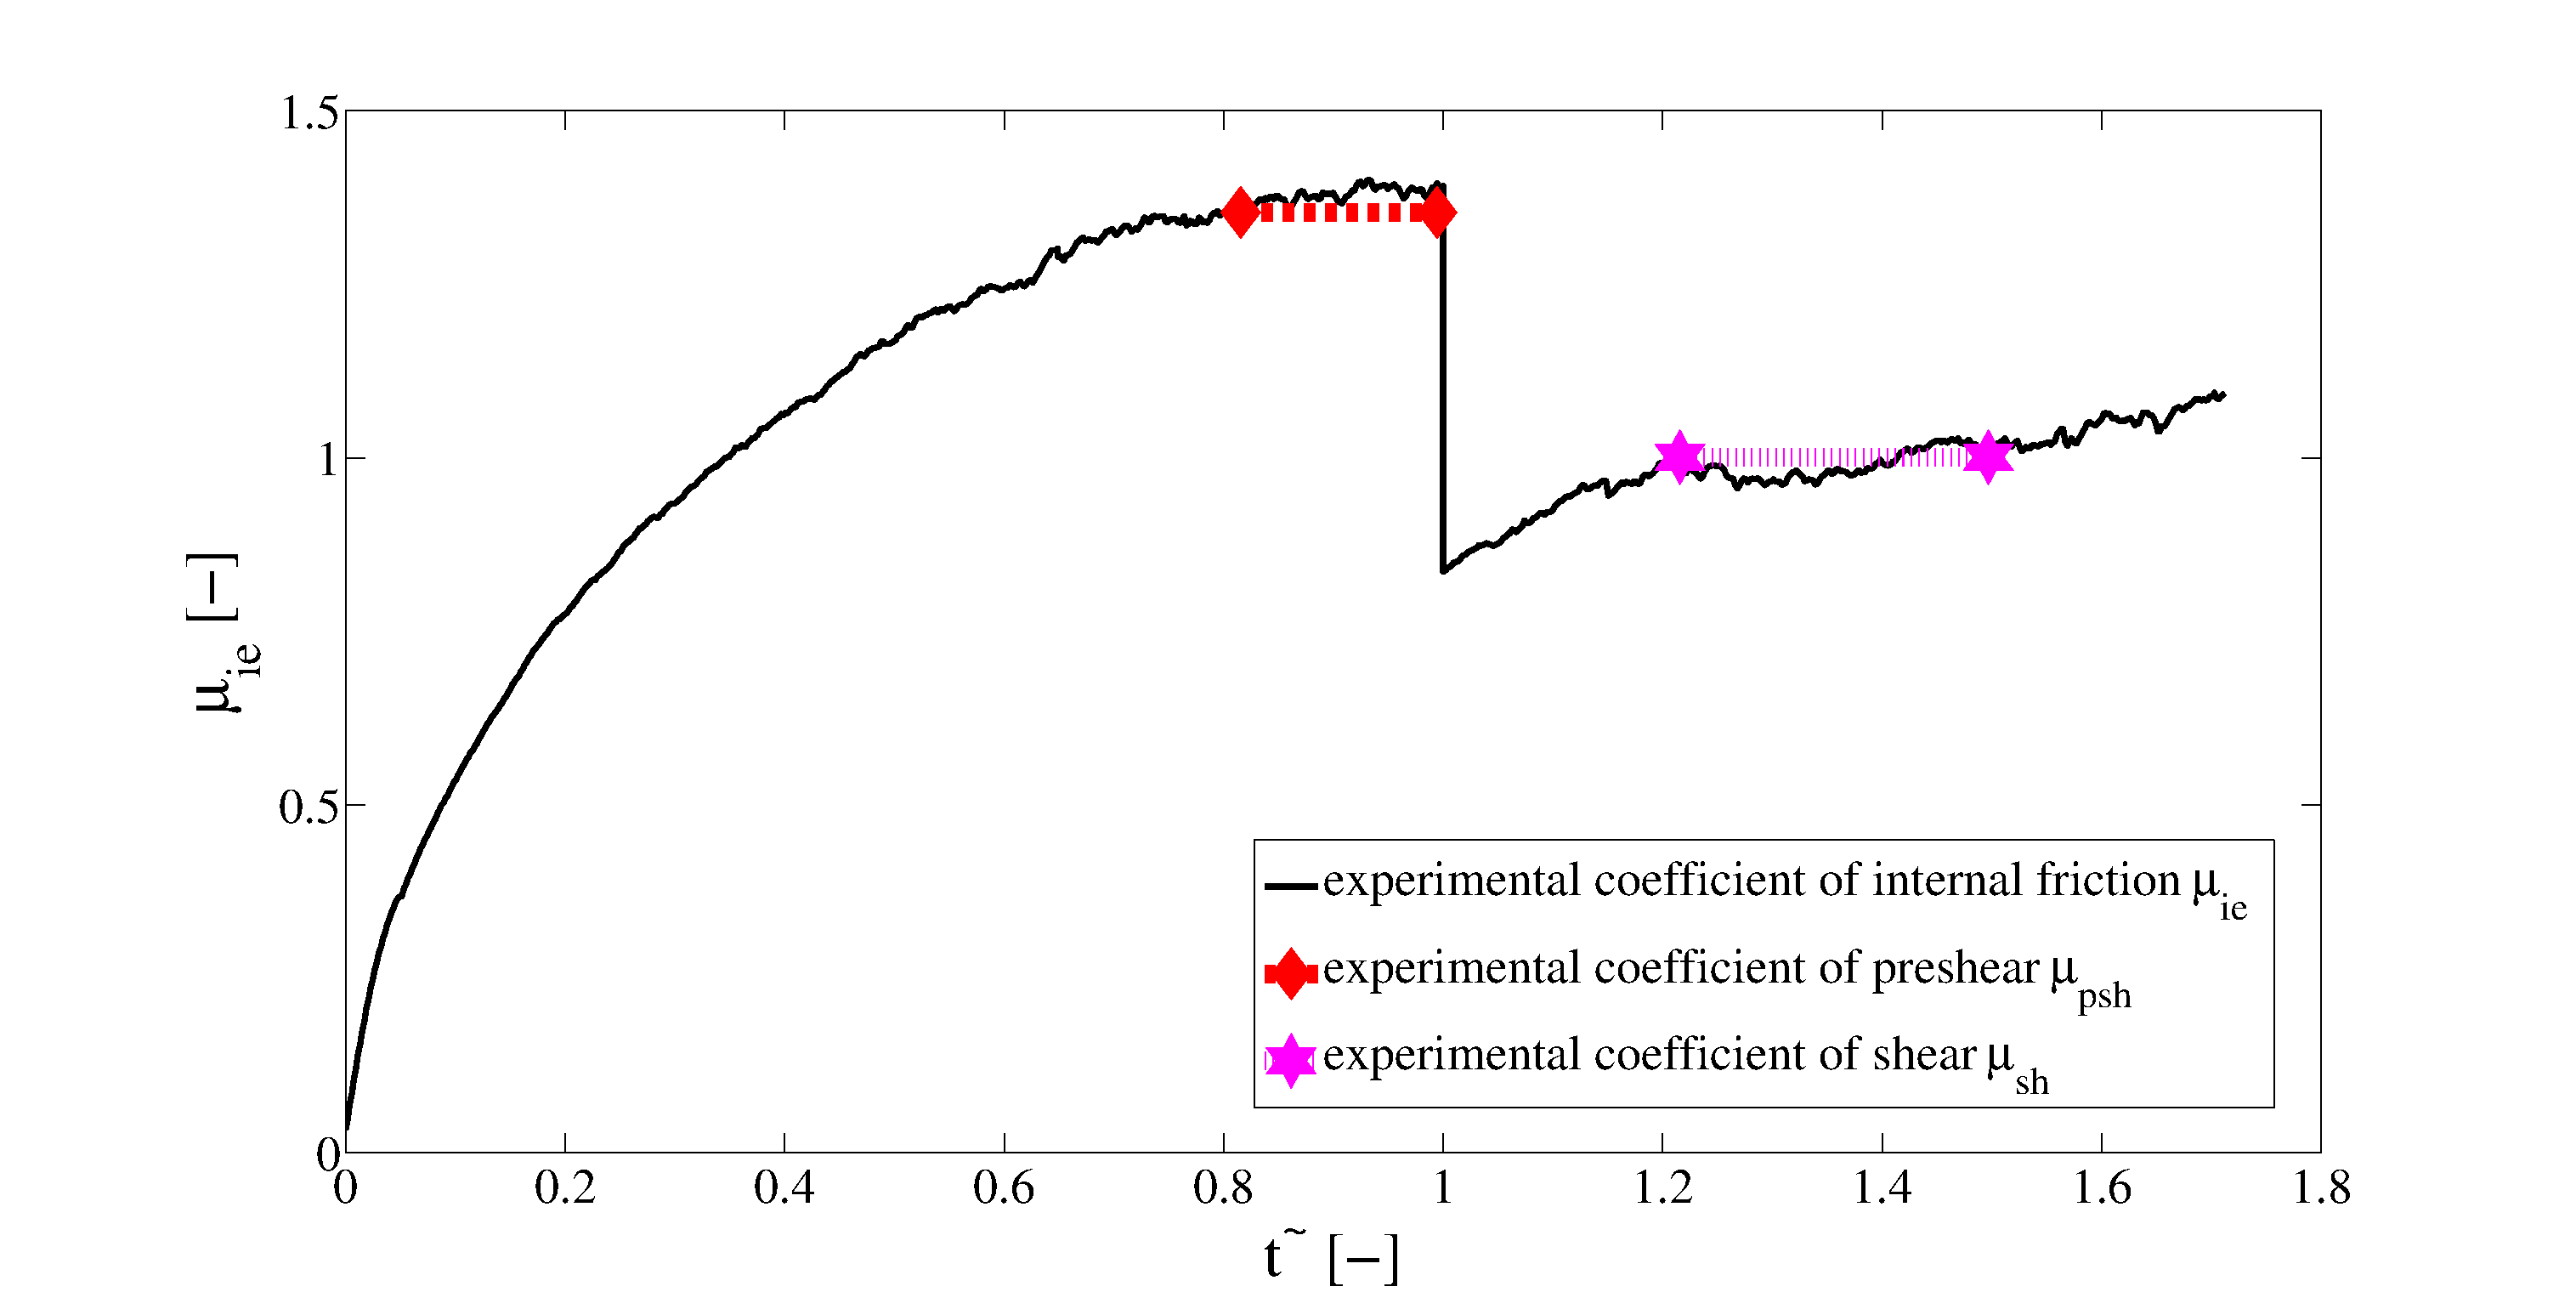
\includegraphics[width=.96\textwidth]{images/original/20experimental} 
\caption{Experimental stress path}
\label{fig:20experimental} 
\end{figure}


% \begin{figure}[htp]
%     \centering
%     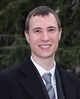
\includegraphics[width=.2\textwidth]{images/vitae/lbenvenuti}
%     \caption{OpenMP, MPI, MPI/OpenMP Hybrid runs of Box in a box testcase on 32
%     cores. The OpenMP-only run suffers from limited memory bandwidth in
%     memory-bound algorithms inside of the Modify section of the code. MPI-only has
%     low averaged runtimes for each section, but a very large Other timing, which
%     hints for a large amount of load-imbalance. Hybrid timings are a bit worse
%     on average, but because of better balancing, processes have lower wait times
%     inside of Other timing.}
% 	\label{fig:boxInBoxComparison}


\subsection{DEM Simulations}
\label{subsec:simulations}

For sinter fine 546 shear cell and 81 static angle of repose simulations have
been realized with the variation described in Tab.
\ref{tab:10DEMVariableinputvalues}.
A representative stress path can be seen in Fig. \ref{fig:21simexample}.
The computational time resulted in 1 hour with 32 AMD cores for a benchmark
shear cell simulation and 9 hours for a benchmark $AOR$ simulation, both with 50K particles. 
Simulations with large $dCylDp$ required a greater time amount (e.g. with 400K
particles (about 12 hours for the shear cell). \\
\begin{figure}[!htb] 
\centering 
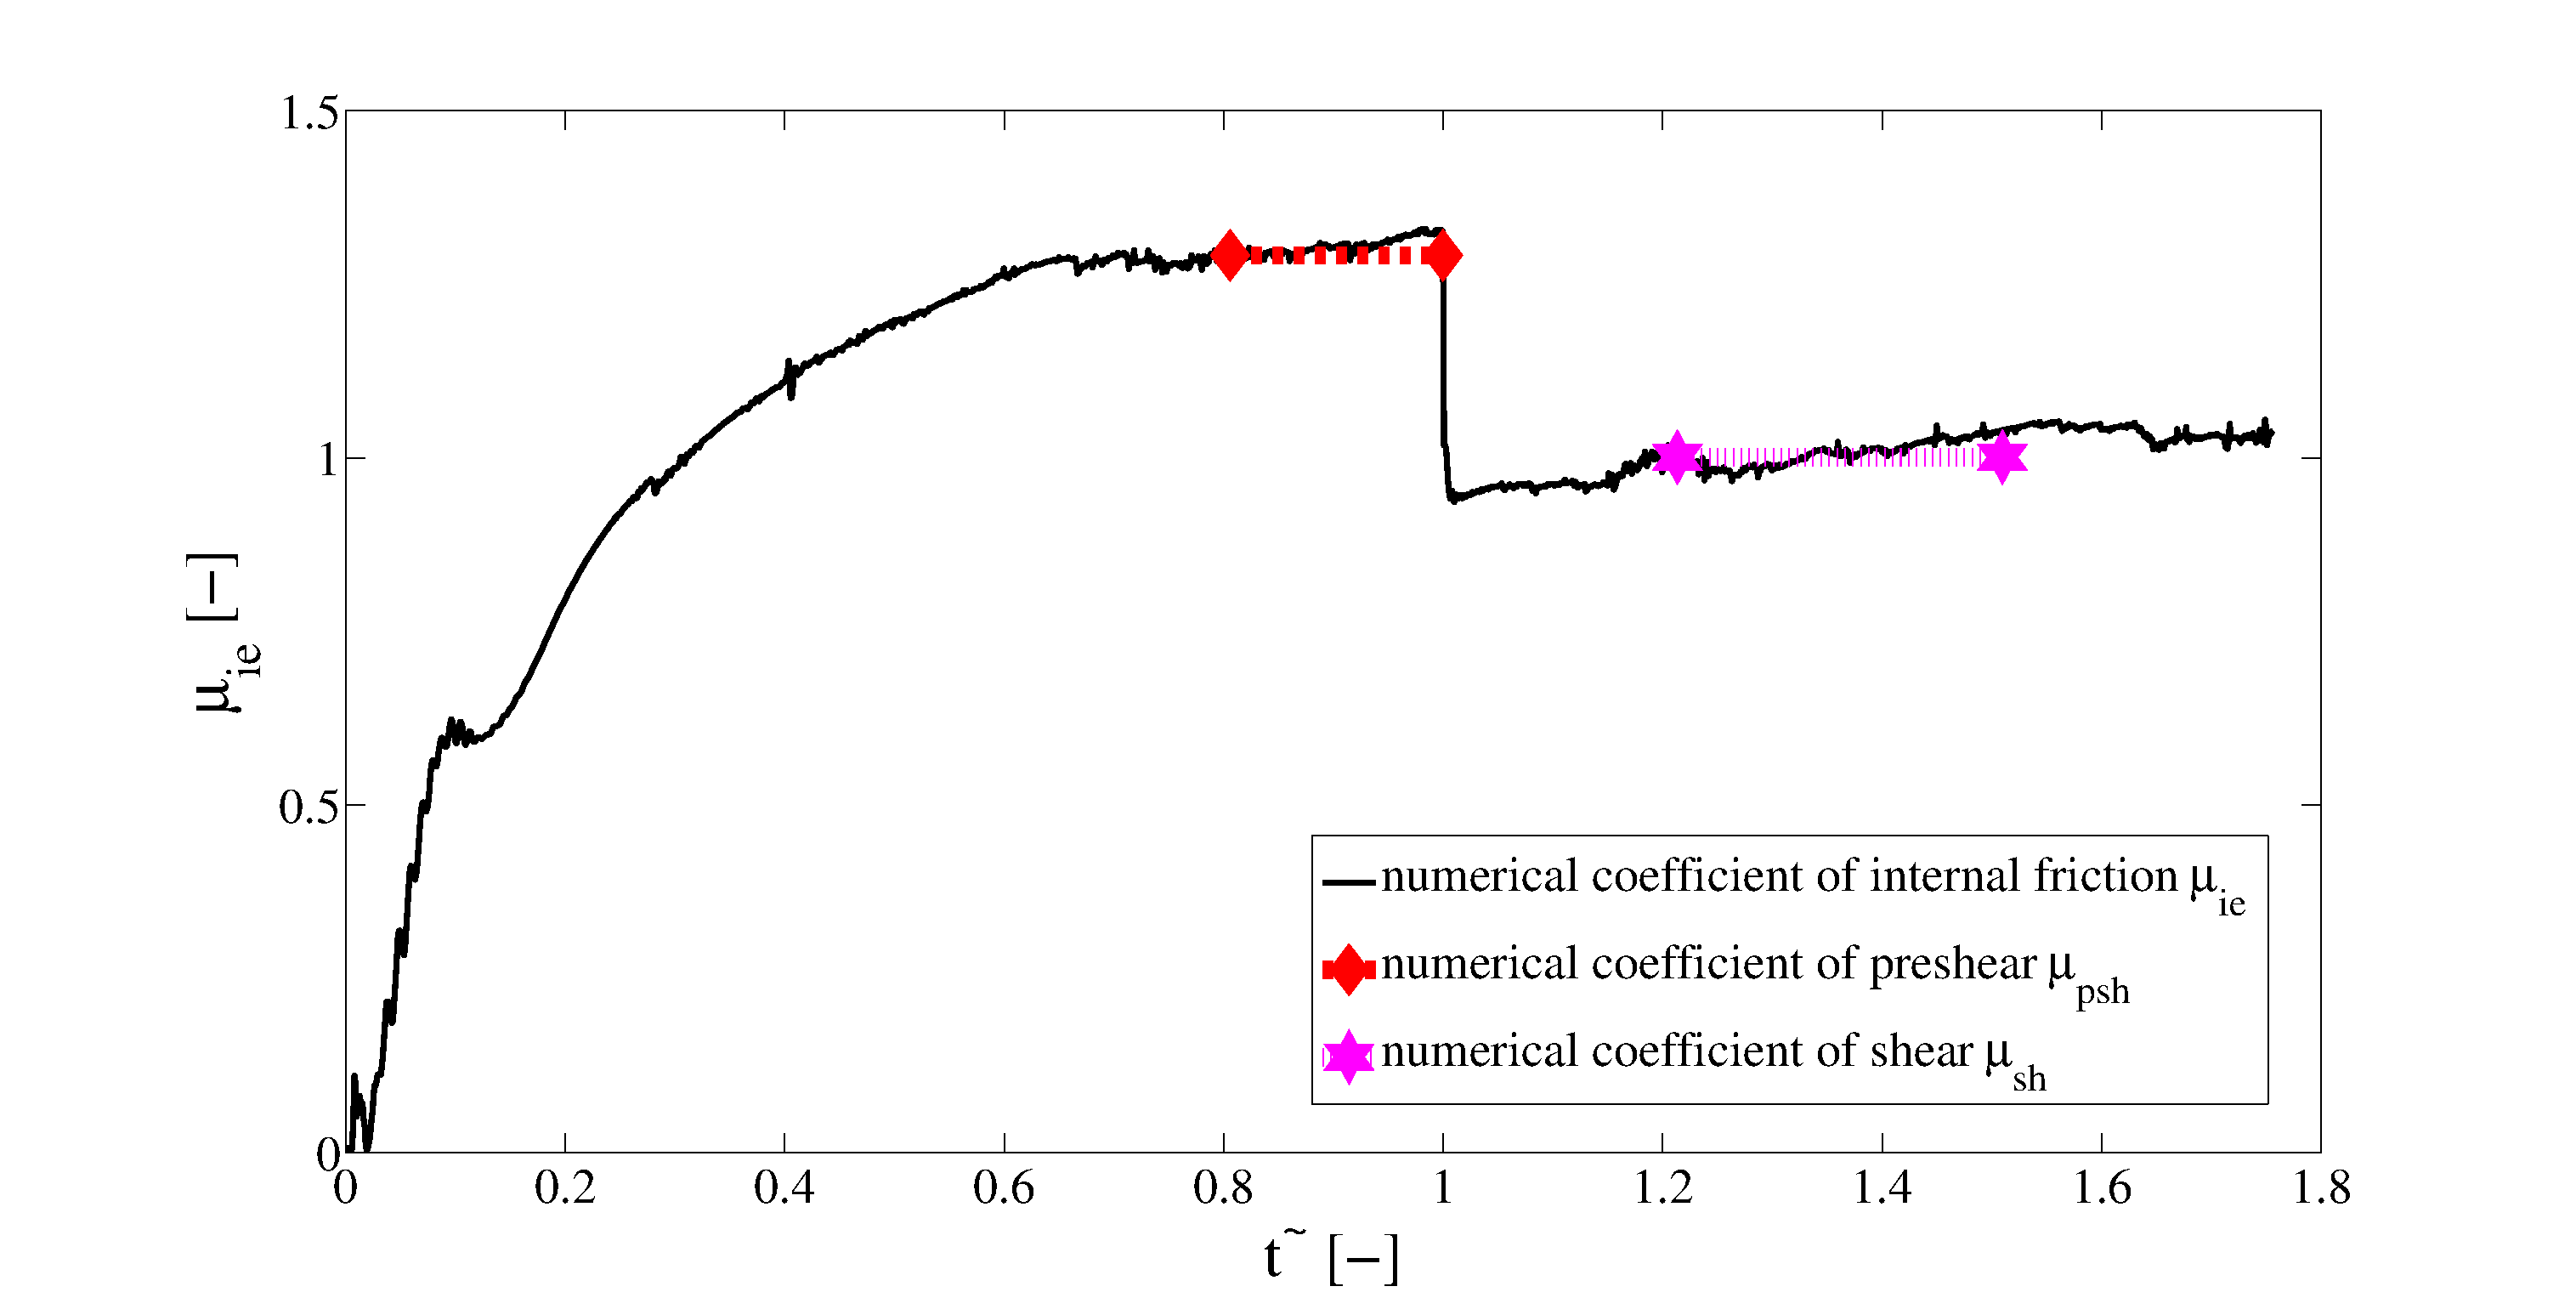
\includegraphics[width=.96\textwidth]{images/original/21simexample} 
\caption{Numerical stress path}
\label{fig:21simexample} 
\end{figure}


% \begin{figure}[htp]
%     \centering
%     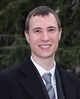
\includegraphics[width=.2\textwidth]{images/vitae/lbenvenuti}
%     \caption{OpenMP, MPI, MPI/OpenMP Hybrid runs of Box in a box testcase on 32
%     cores. The OpenMP-only run suffers from limited memory bandwidth in
%     memory-bound algorithms inside of the Modify section of the code. MPI-only has
%     low averaged runtimes for each section, but a very large Other timing, which
%     hints for a large amount of load-imbalance. Hybrid timings are a bit worse
%     on average, but because of better balancing, processes have lower wait times
%     inside of Other timing.}
% 	\label{fig:boxInBoxComparison}


\subsection{ANN model development}
\label{subsec:annmodeldev}

First, we present the regression plot of a bulk behaviour parameter, e.g. the
$\mu_{e-psh}$, see Fig. \ref{fig:22regression}, where the regression plot for
the $NN$ with the maximum $R^2$ in shown. Each circle represents a simulation. 
The plot presents a consistent agreement between the $DEM$ results distribution and the $NN$ regression line.
% \begin{figure}%[!h] 
\centering 
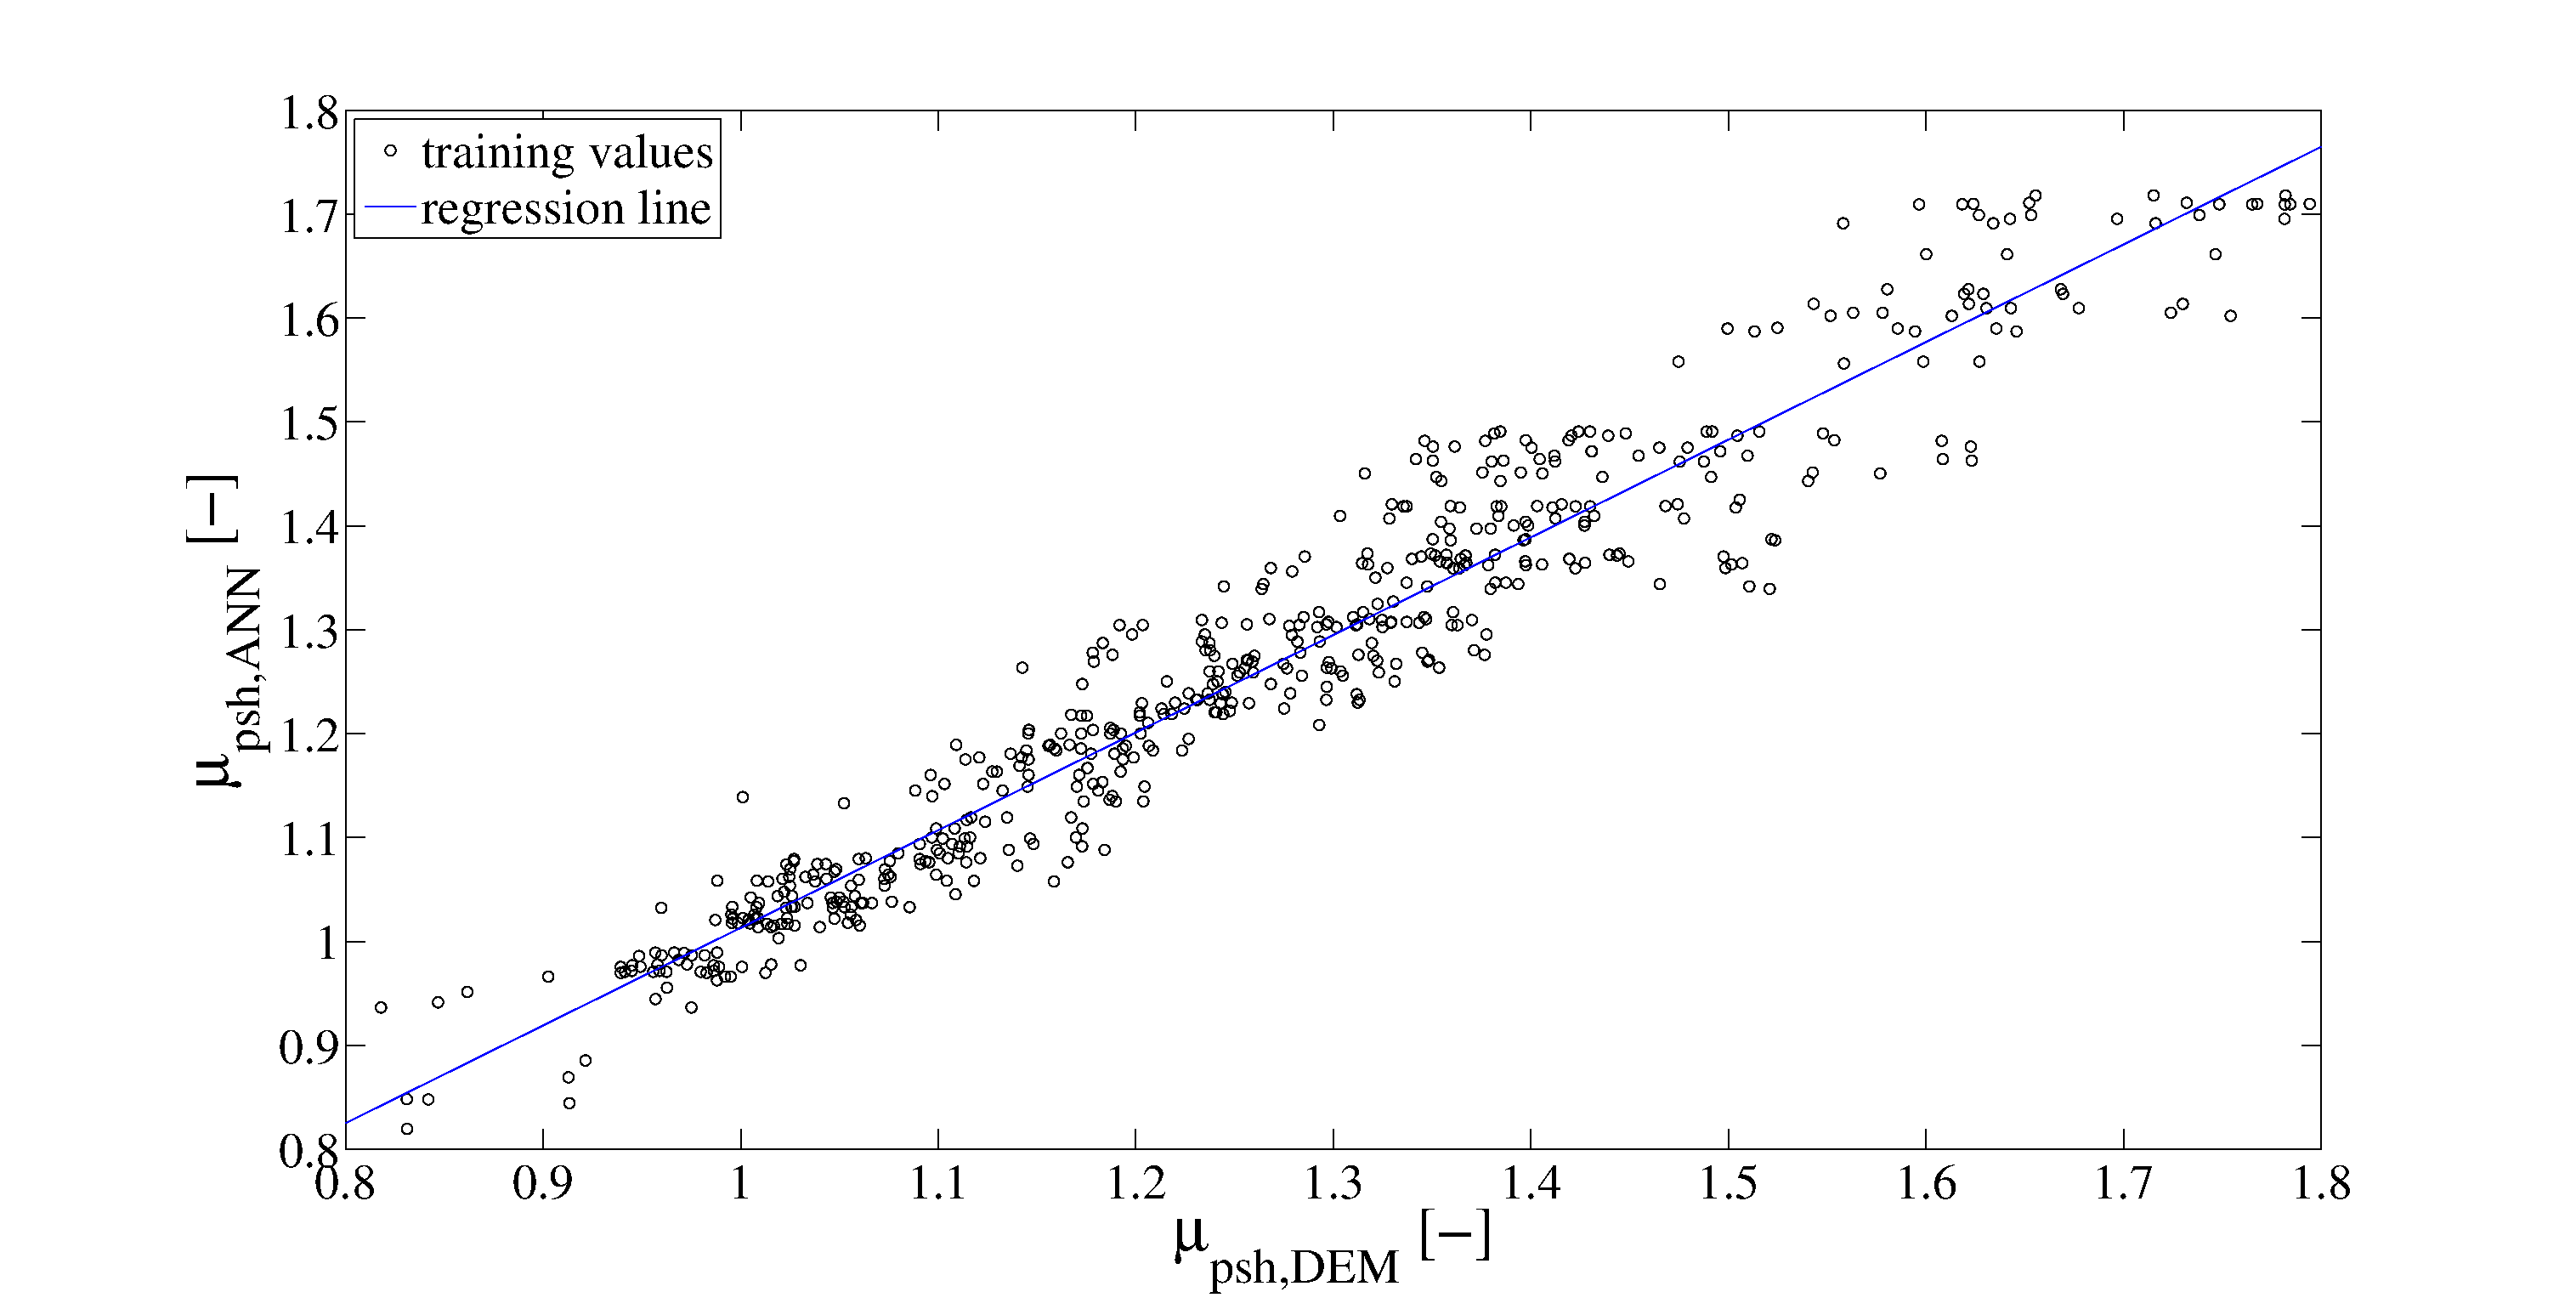
\includegraphics[width=.96\columnwidth]{images/22regression.eps}
%[width=.96\textwidth]
\caption[Comparison between prediction of the trained ANN and full DEM
simulation]{Comparison between prediction of the trained Artificial Neural
Network ($ANN$) and 546 
\wrong{write down all the simulations performed at the end.}
full DEM simulations of the coefficient of pre-shear
($\mu_{psh}$).}
\label{fig:22regression} 
\end{figure}
The linear relationship between the
training values have been evaluated in Table \ref{tab:06inputRelationshipTable}.
% \begin{table}[h]
\centering
\scalebox{1.0}{
\begin{tabular}{c|cccccccc}
\hline
          & $\mu_s$ & $\mu_r$ & $COR$ & $\rho_p$ & $\mu_{sh}$ & $\mu_{psh}$ & $\rho_{b}$ & $AOR$ \\
          \hline
    $\mu_s$ & 100.00 & 0.55  & 0.04  & 0.00  & 3.84  & 87.26 & 8.39  & 49.48 \\
    $\mu_r$ & 0.55  & 100.00 & 0.15  & 0.00  & 58.92 & 33.70 & 3.10  & 60.20 \\
    $COR$ & 0.04  & 0.15  & 100.00 & 0.00  & 15.52 & 0.57  & 1.71  & 0.00 \\
    $\rho_p$ & 0.00  & 0.00  & 0.00  & 100.00 & 4.98  & 5.71  & 99.00 & 0.00 \\
    $\mu_{sh}$ & 3.84  & 58.92 & 15.52 & 4.98  & 100.00 & 26.03 & 9.52  & 0.00 \\
    $\mu_{psh}$ & \textbf{87.26} & 33.70 & 0.57  & 5.71  & 26.03 & 100.00 & 4.33 
    & 0.00
    \\
    $\rho_{b}$ & 8.39  & 3.10  & 1.71  & \textbf{99.00} & 9.52  & 4.33  & 100.00
    & 0.00 \\
    $AOR$ & 49.48 & \textbf{60.20} & 0.00  & 0.00  & 0.00  & 0.00  & 0.00  &
    100.00 \\
    
\hline
\end{tabular}}
\caption{Values of linear relationship between considered variables multiplied
for 100}
\label{tab:06inputRelationshipTable}
\end{table}
Then we show how the $R^2$ changed with the different number of neurons. The
straight line, referred only to the test simulations, is more sensible to
variations of number of neurons, see Fig. \ref{fig:23regressiongraph}, compared
to the total line. In the latter, also the correlated simulations used for
training participate in the $R^2$ evaluation.
% \begin{figure}[!h] 
\centering 
\includegraphics[width=.96\textwidth]{images/original/23regressiongraph}
%[width=.96\textwidth]
\caption{Regression graph}
\label{fig:23regressiongraph} 
\end{figure}


% \begin{figure}[htp]
%     \centering
%     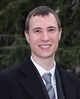
\includegraphics[width=.2\textwidth]{images/vitae/lbenvenuti}
%     \caption{OpenMP, MPI, MPI/OpenMP Hybrid runs of Box in a box testcase on 32
%     cores. The OpenMP-only run suffers from limited memory bandwidth in
%     memory-bound algorithms inside of the Modify section of the code. MPI-only has
%     low averaged runtimes for each section, but a very large Other timing, which
%     hints for a large amount of load-imbalance. Hybrid timings are a bit worse
%     on average, but because of better balancing, processes have lower wait times
%     inside of Other timing.}
% 	\label{fig:boxInBoxComparison}

Thus, we selected the $NN$ with the maximum $R^2$ in the test line, as stated in the methodology.
Later, we processed the random combinations (Tab.
\ref{tab:10DEMVariableinputvalues}) with the $NN$.
The $NN$ evaluation was incredibly faster compared to the $DEM$ simulations. The
individuation of all the tabbed $DEM$ combinations for the shear cell did not take more than a few seconds on a single core. 
We represented the tabbed combinations for one load condition of the shear cell in Fig.
\ref{fig:24radarpirker1schulze10070}.
% \begin{figure}[htp] \centering
    \begin{subfigure}[b]{0.48\columnwidth}
        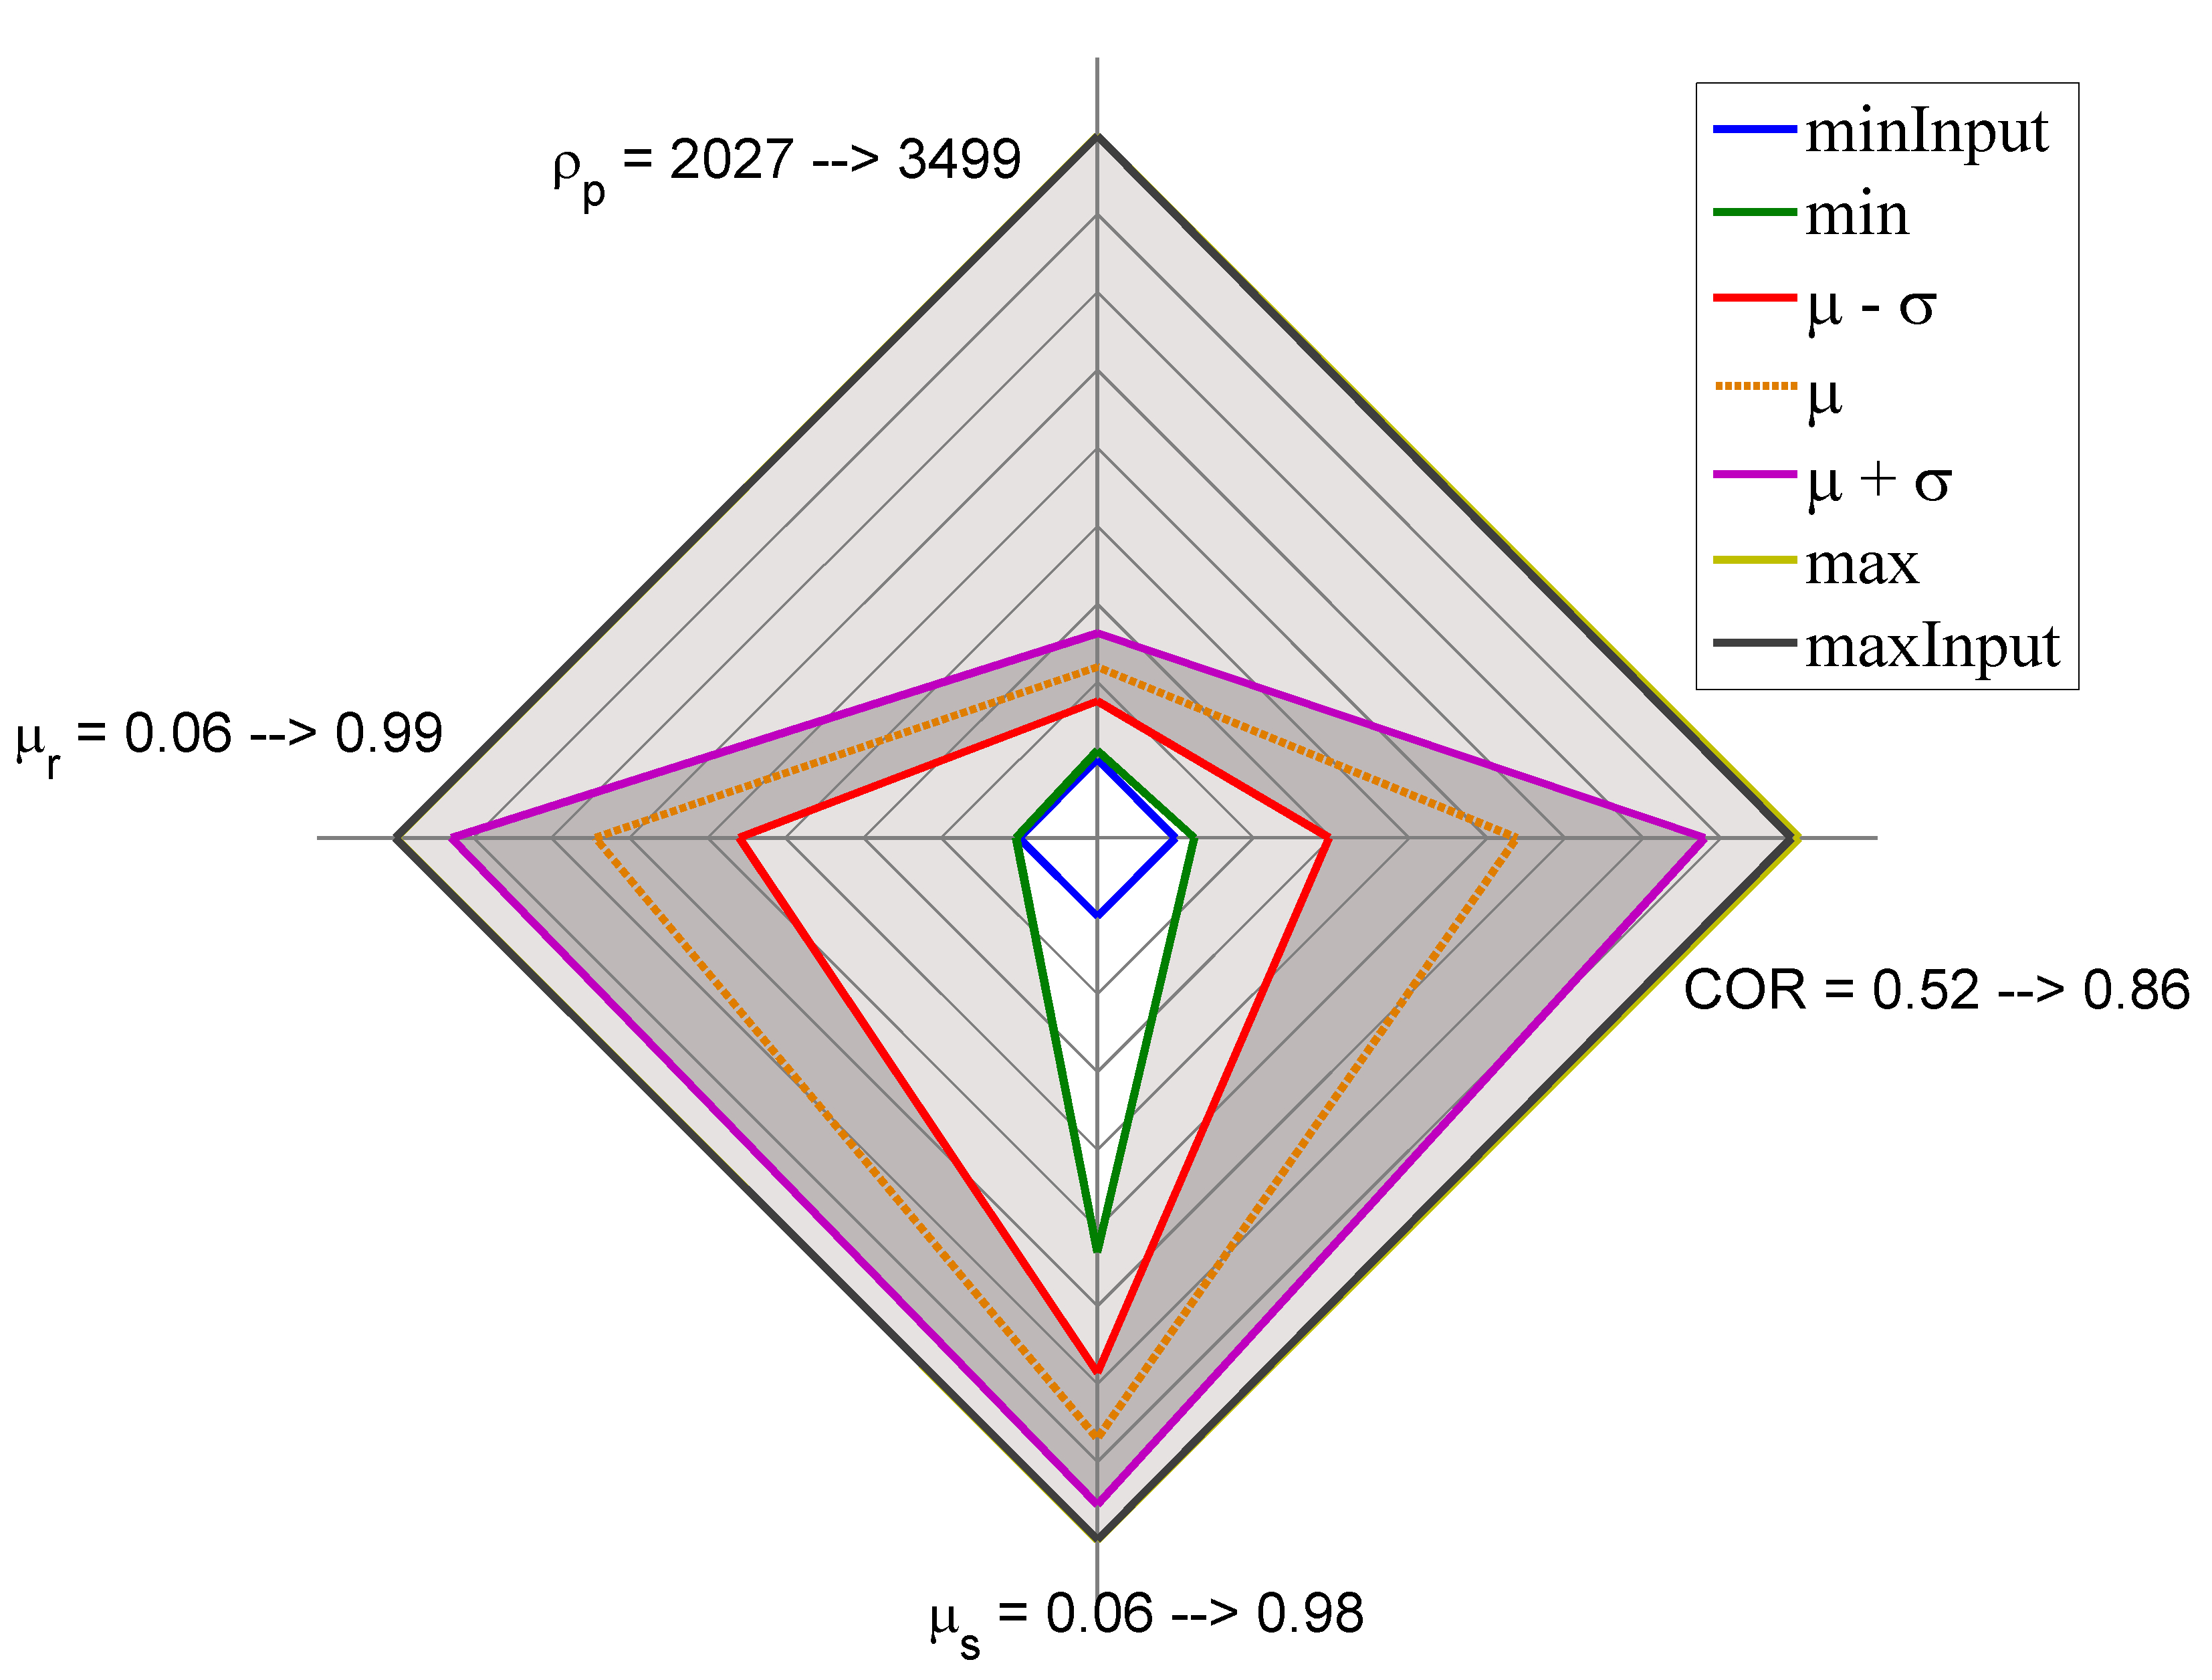
\includegraphics[width=\textwidth]{images/original/24radarpirker1schulze10070}
        \caption{Radar P1 Schulze10070}
        \label{fig:24radarpirker1schulze10070}
    \end{subfigure}
    \begin{subfigure}[b]{0.48\columnwidth}
        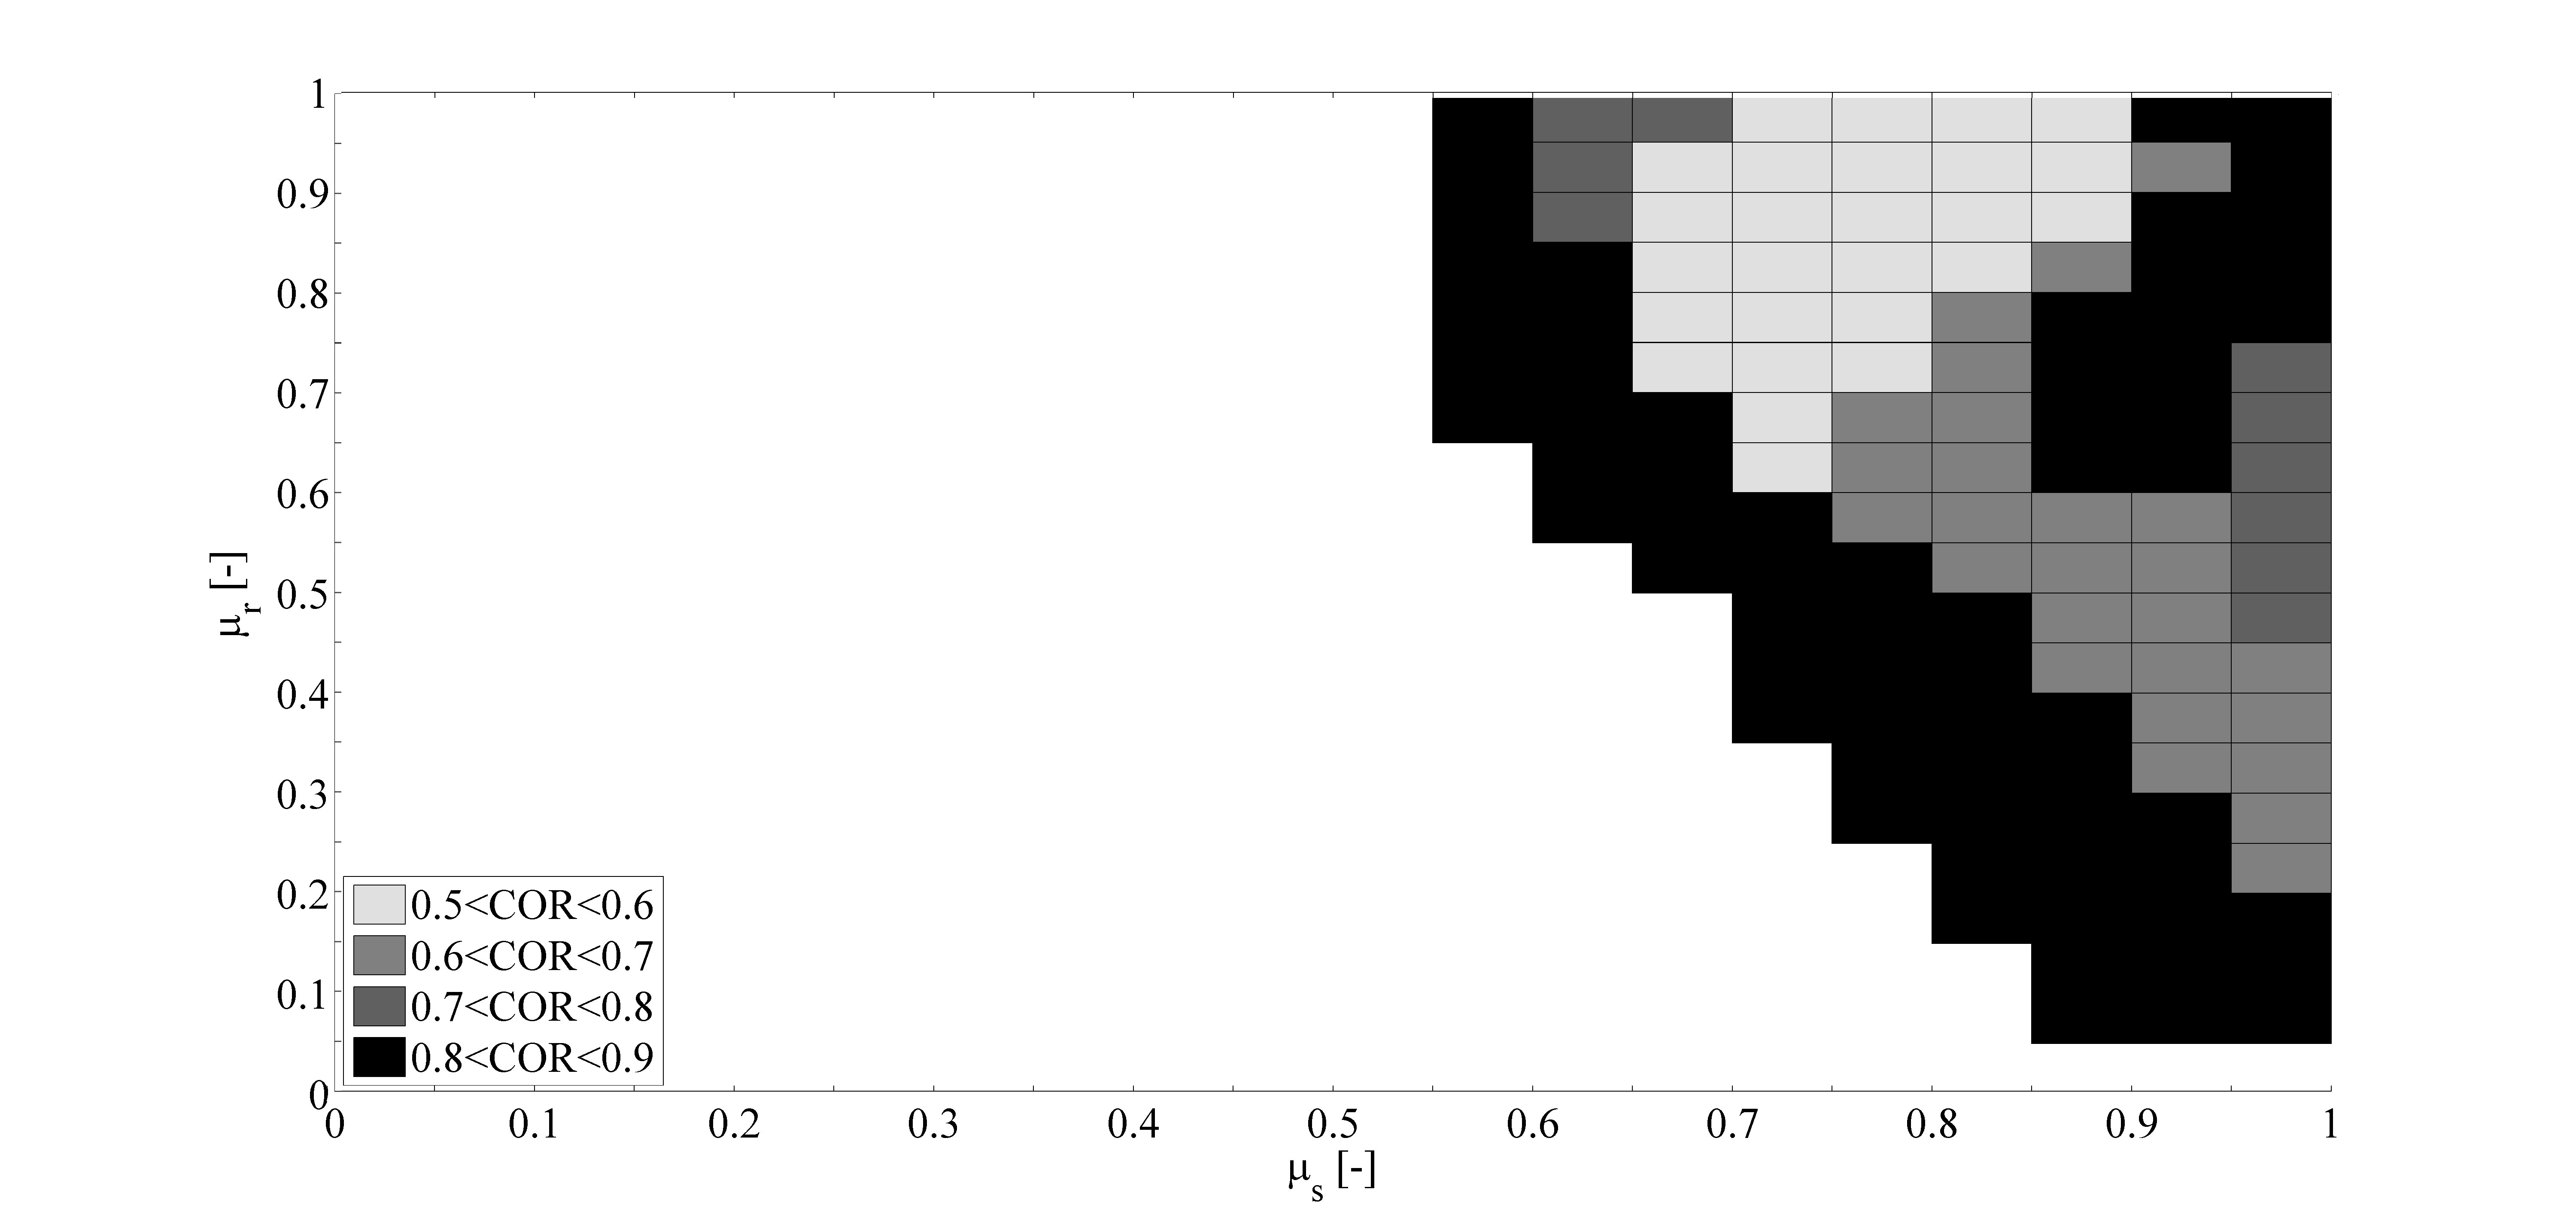
\includegraphics[width=\textwidth]{images/original/25cloudpirker1schulze10070}
        \caption{Cloud P1 Schulze10070}
        \label{fig:25cloudpirker1schulze10070}
    \end{subfigure}\\
        \begin{subfigure}[b]{0.48\columnwidth}
        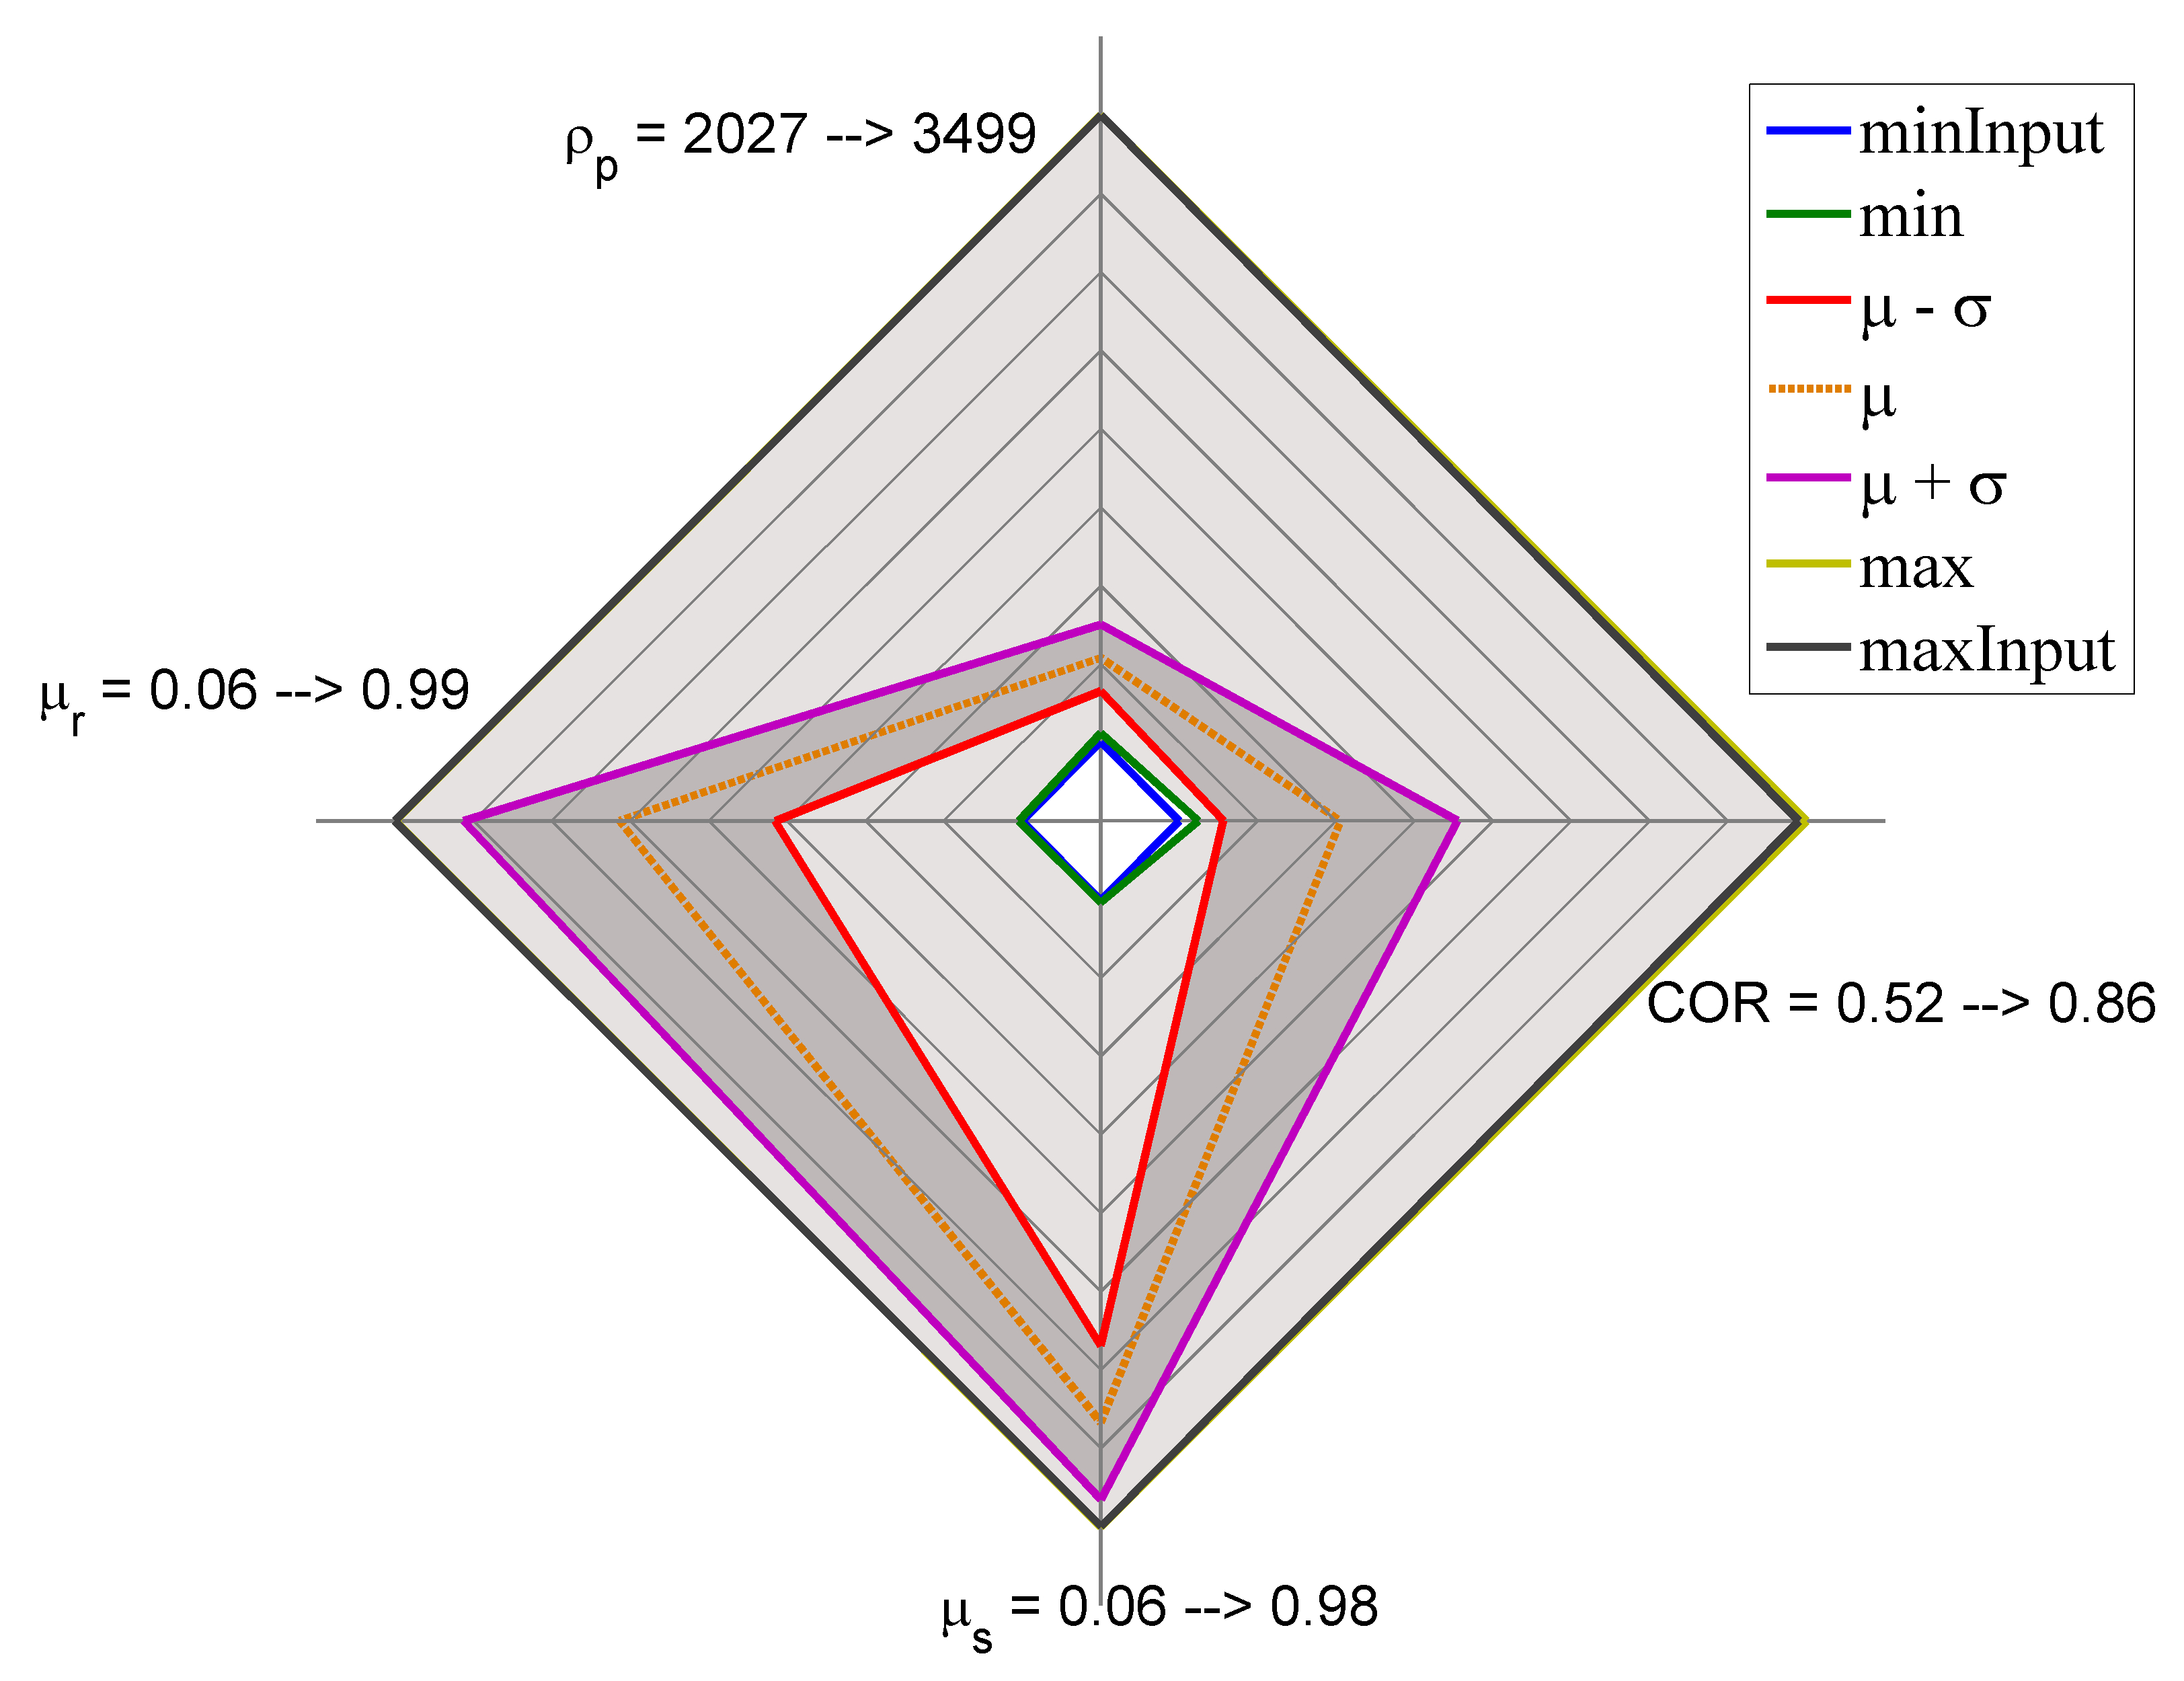
\includegraphics[width=\textwidth]{images/original/26radarpirker08schulze10070}
        \caption{Radar P08 Schulze10070}
        \label{fig:26radarpirker08schulze10070} 
    \end{subfigure}
    \begin{subfigure}[b]{0.48\columnwidth}
        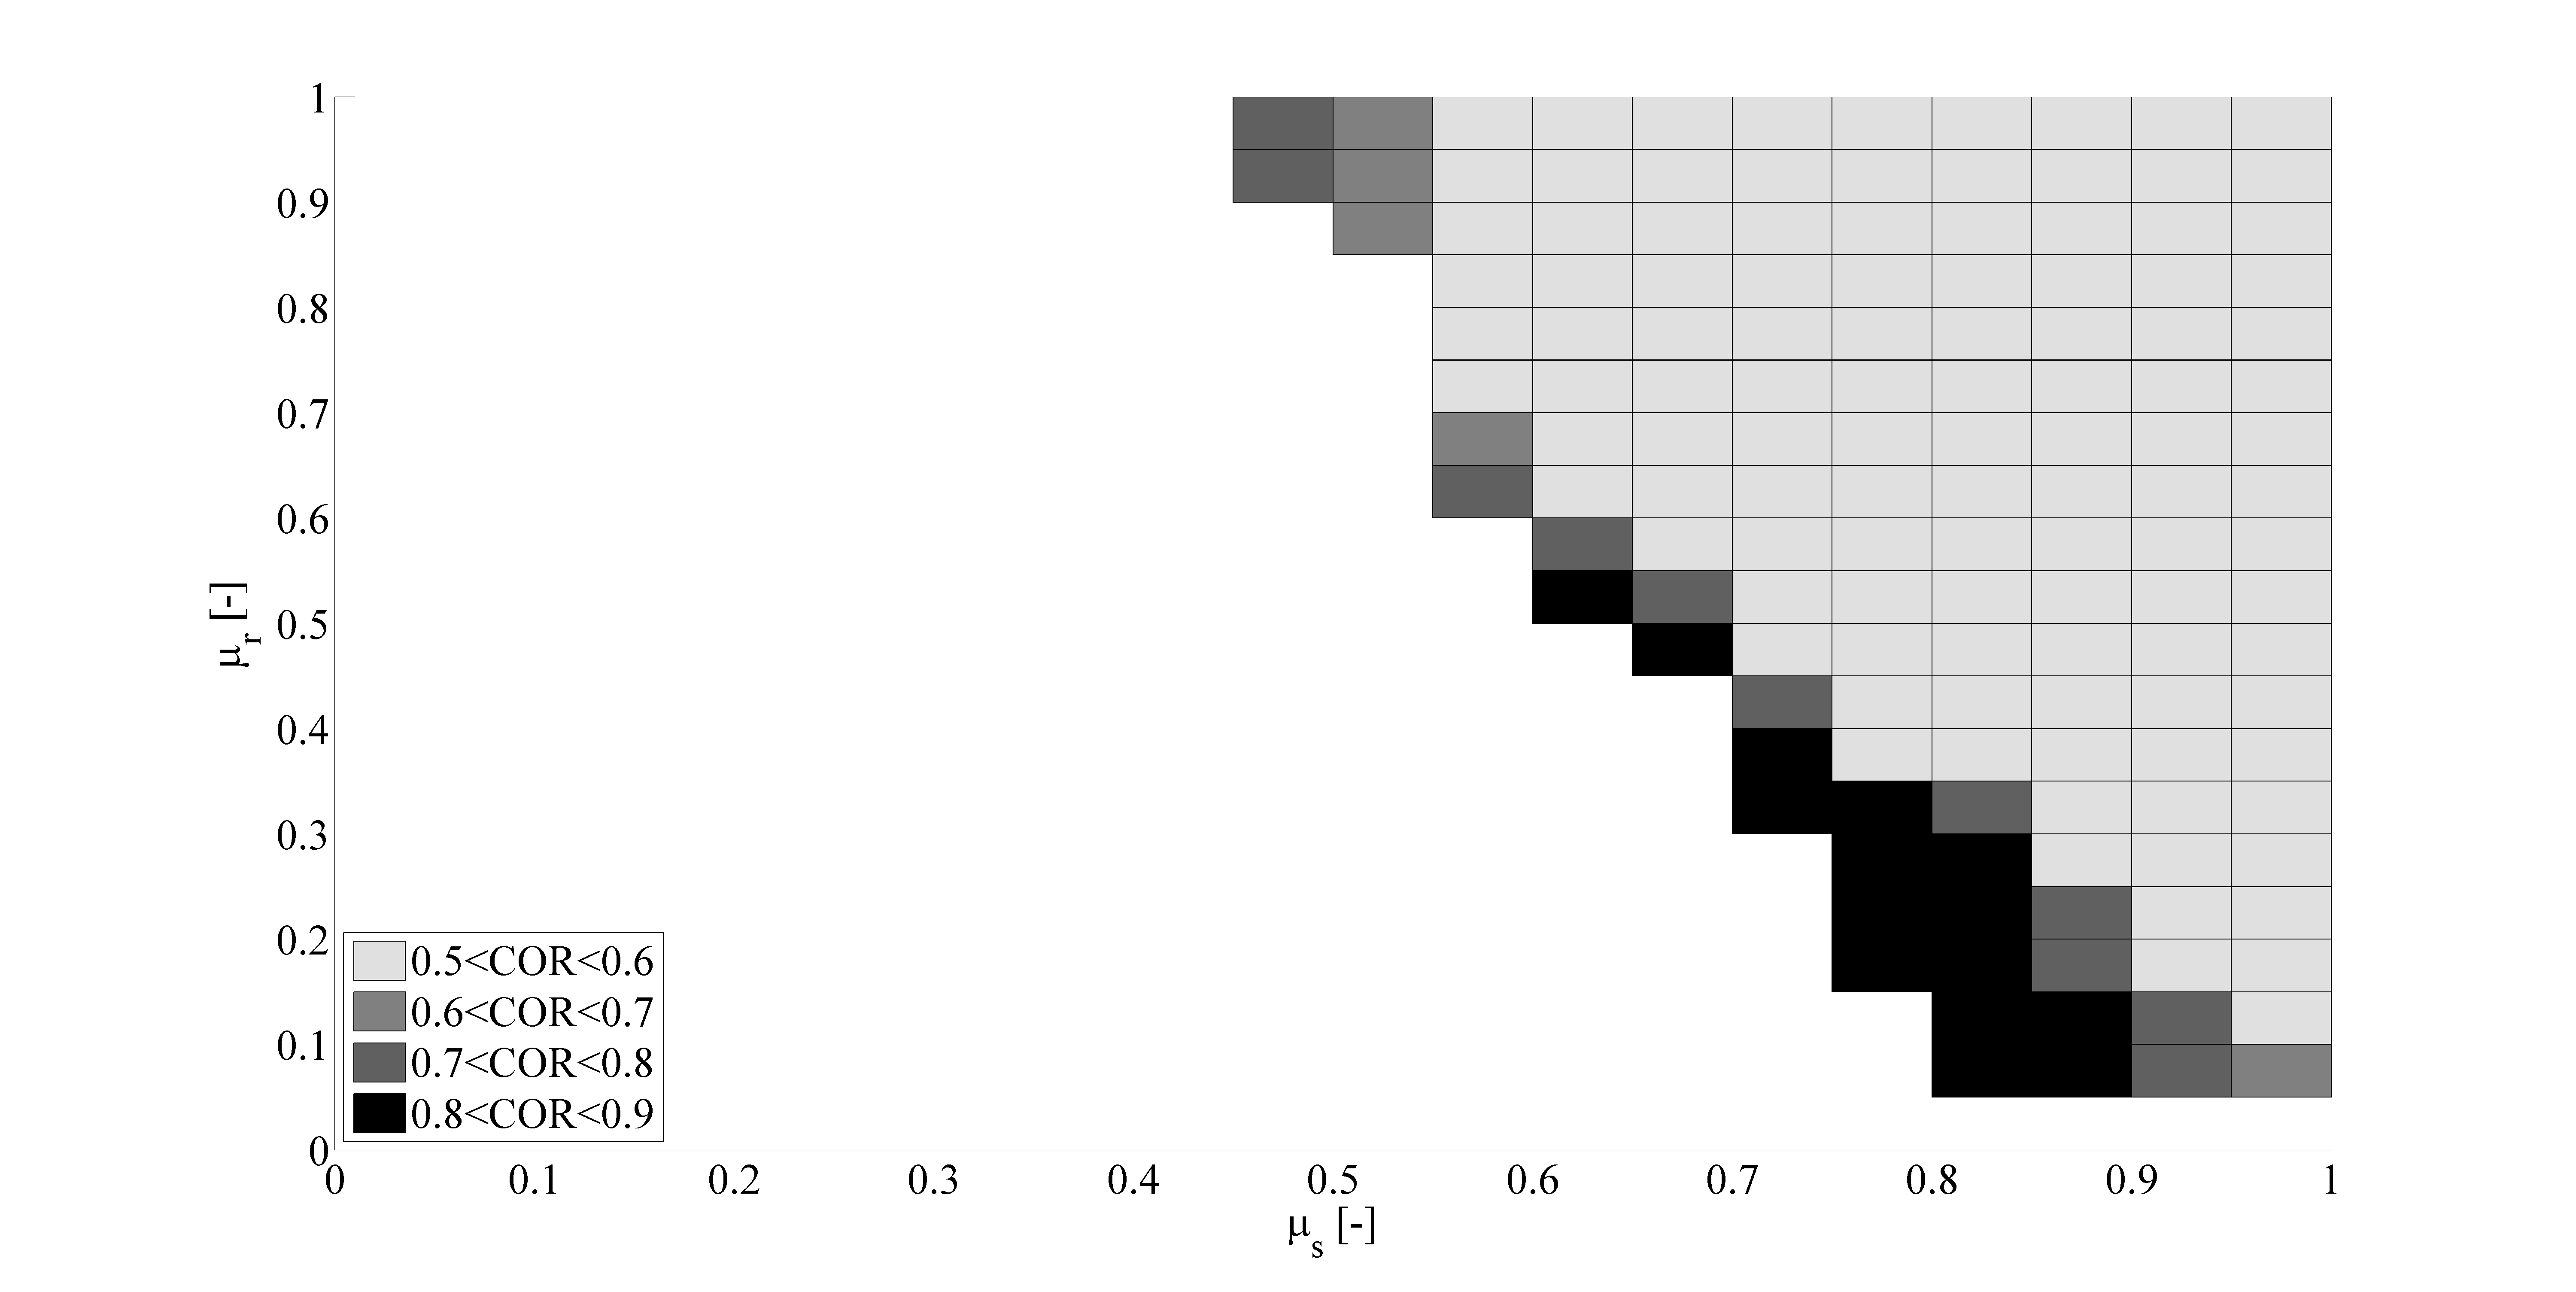
\includegraphics[width=\textwidth]{images/original/27cloudpirker08schulze10070}
        \caption{Cloud P08 Schulze10070}
        \label{fig:27cloudpirker08schulze10070} 
    \end{subfigure}\\
        \begin{subfigure}[b]{0.48\columnwidth}
        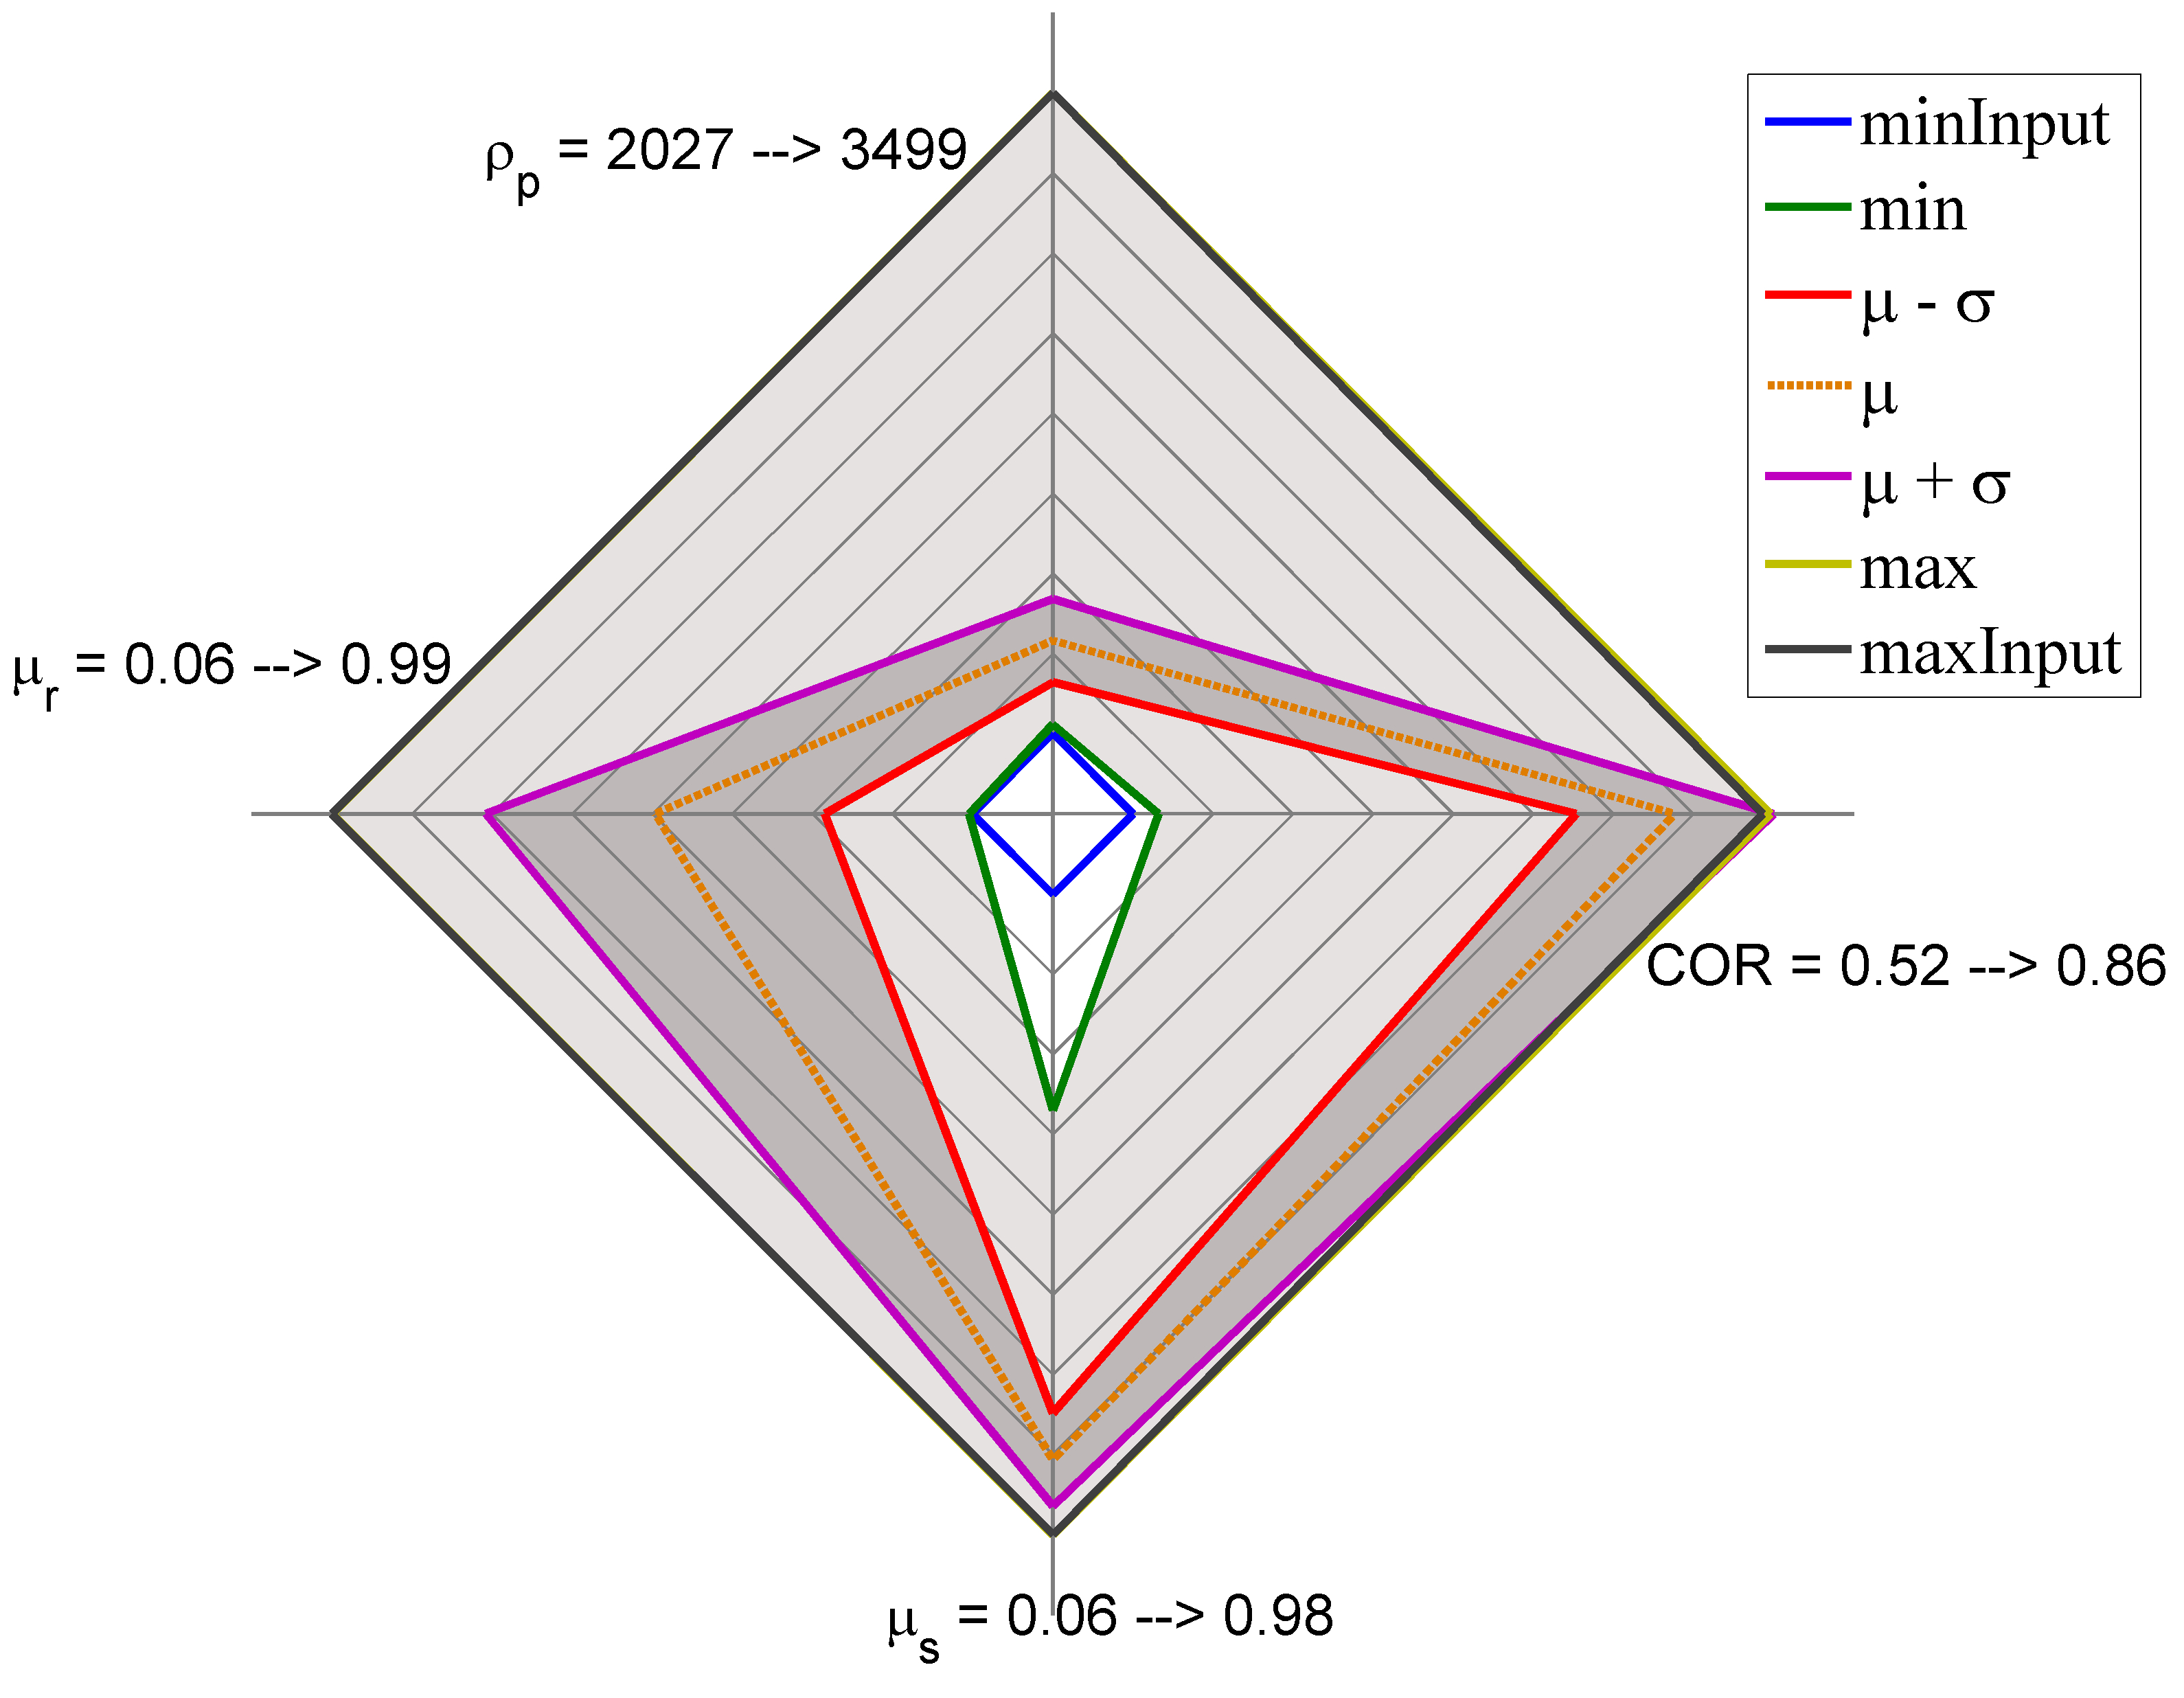
\includegraphics[width=\textwidth]{images/original/28radarpirker12schulze10070}
        \caption{Radar P12 Schulze10070}
        \label{fig:28radarpirker12schulze10070} 
    \end{subfigure}
    \begin{subfigure}[b]{0.48\columnwidth}
        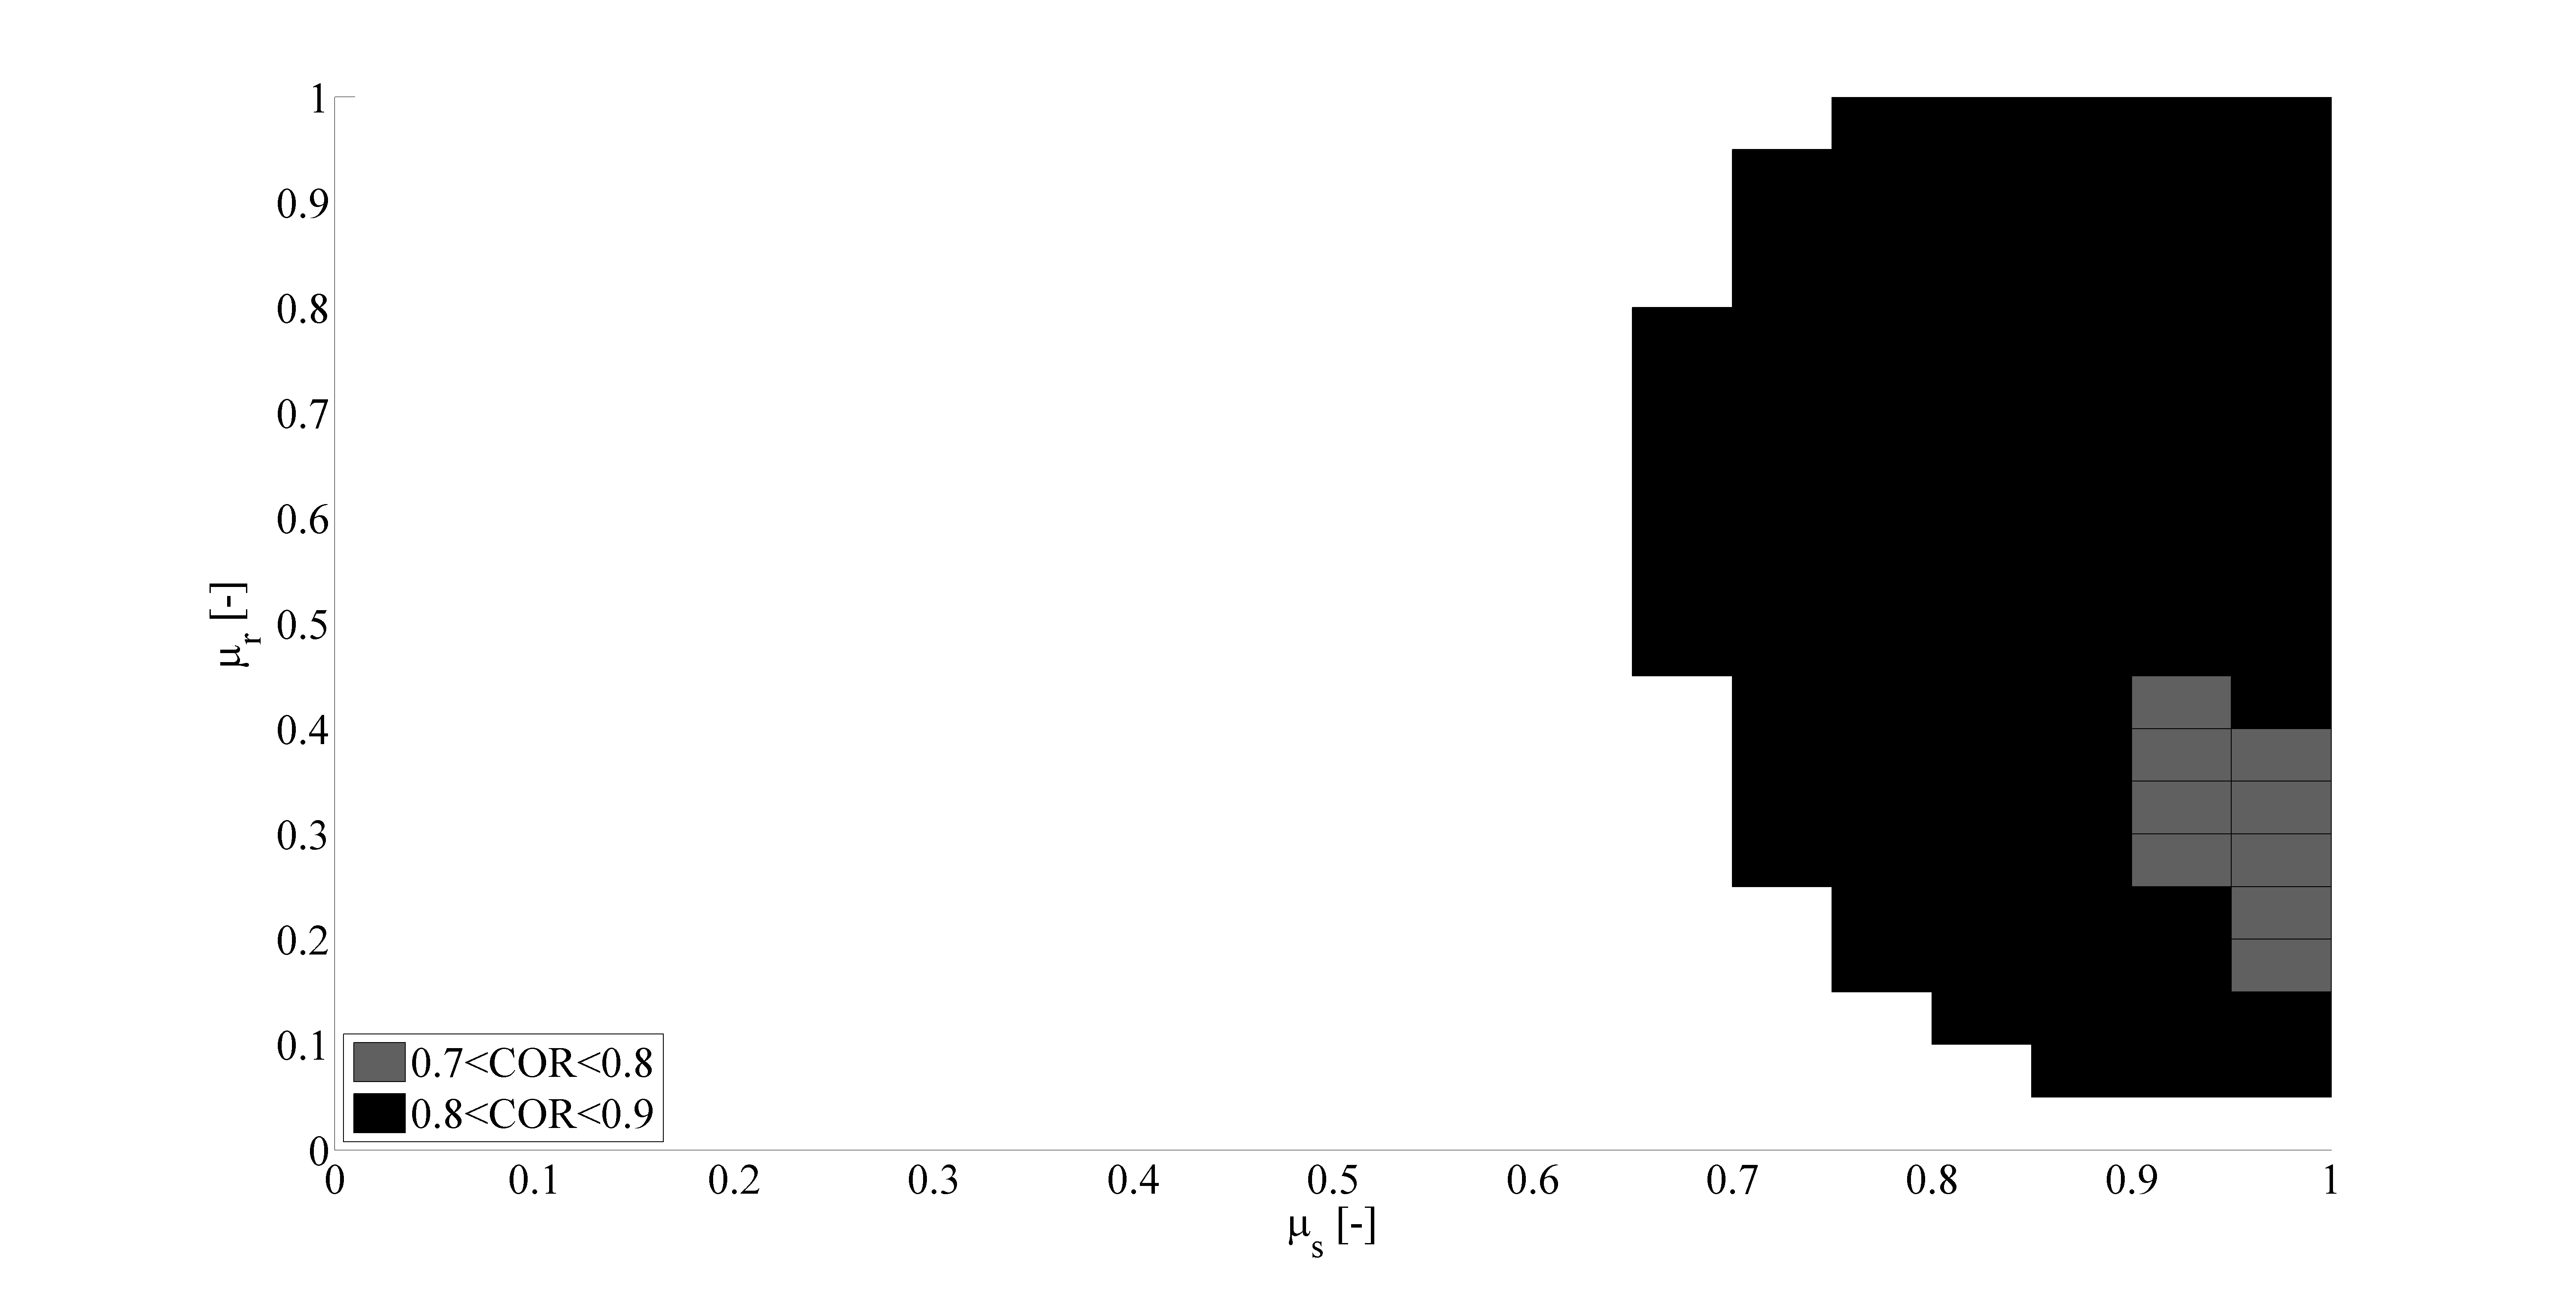
\includegraphics[width=\textwidth]{images/original/30cloudpirker12schulze10070}
        \caption{Cloud P12 Schulze10070}
        \label{fig:30cloudpirker12schulze10070} 
    \end{subfigure}
    \caption{Comparison between the original experimental selection P=1 and the
    increased and decreased results.}
    \label{fig:29schulzeradarandcloud}
\end{figure}
Here, the minimum and maximum values, together with the mean and the confidence
range, provided by the square deviation, are shown. Notably, the confidence range is large, 
especially for the $COR$, highlighting its scarce influence over the characterization. 
Instead, both the $\rho_p$  and the $\mu_s$ show a narrow confidence range, 
displaying at the same time their influence and the validity of this procedure to find valid $DEM$ parameters. 
Especially, we could see how different $DEM$ parameters combinations could reproduce the experimental 
behaviour and evaluate their mutual dependencies. 
This is clearer in a cloud plot, as in Fig. 
\ref{fig:25cloudpirker1schulze10070}. While the $COR$ varied, multiple
combinations ($250407 --> 4\% $ of the total) of $\mu_s$ and $\mu_r$ reproduced
the experimental behaviour.
This underlines once more their correlation, as already stated by Wensrich and 
Katterfeld \cite{RefWorks:87}.
To further demonstrate the validity of the procedure, we modified the product
coefficient. In the first attempt we set it to $P=0.8$. We can see in the radar plot in Fig. 
\ref{fig:26radarpirker08schulze10070} that the confidence range is narrower
compared to $P=1.0$. Instead in the cloud plot in Fig. 
\ref{fig:27cloudpirker08schulze10070} the area
looks larger, although slightly less densely populated. Finally, for $P=1.2$ the radar plot in Fig.
\ref{fig:28radarpirker12schulze10070} shows a completely different confidence
range, while the cloud plot in Fig. \ref{fig:30cloudpirker12schulze10070} 
illustrates a smaller area. As expected, the procedure was highly sensible to the variations of the experimental data. 
Thus, it could be effectively handled for a wide range of bulk materials.\\
% \begin{figure}[htp] \centering
    \begin{subfigure}[b]{0.48\columnwidth}
        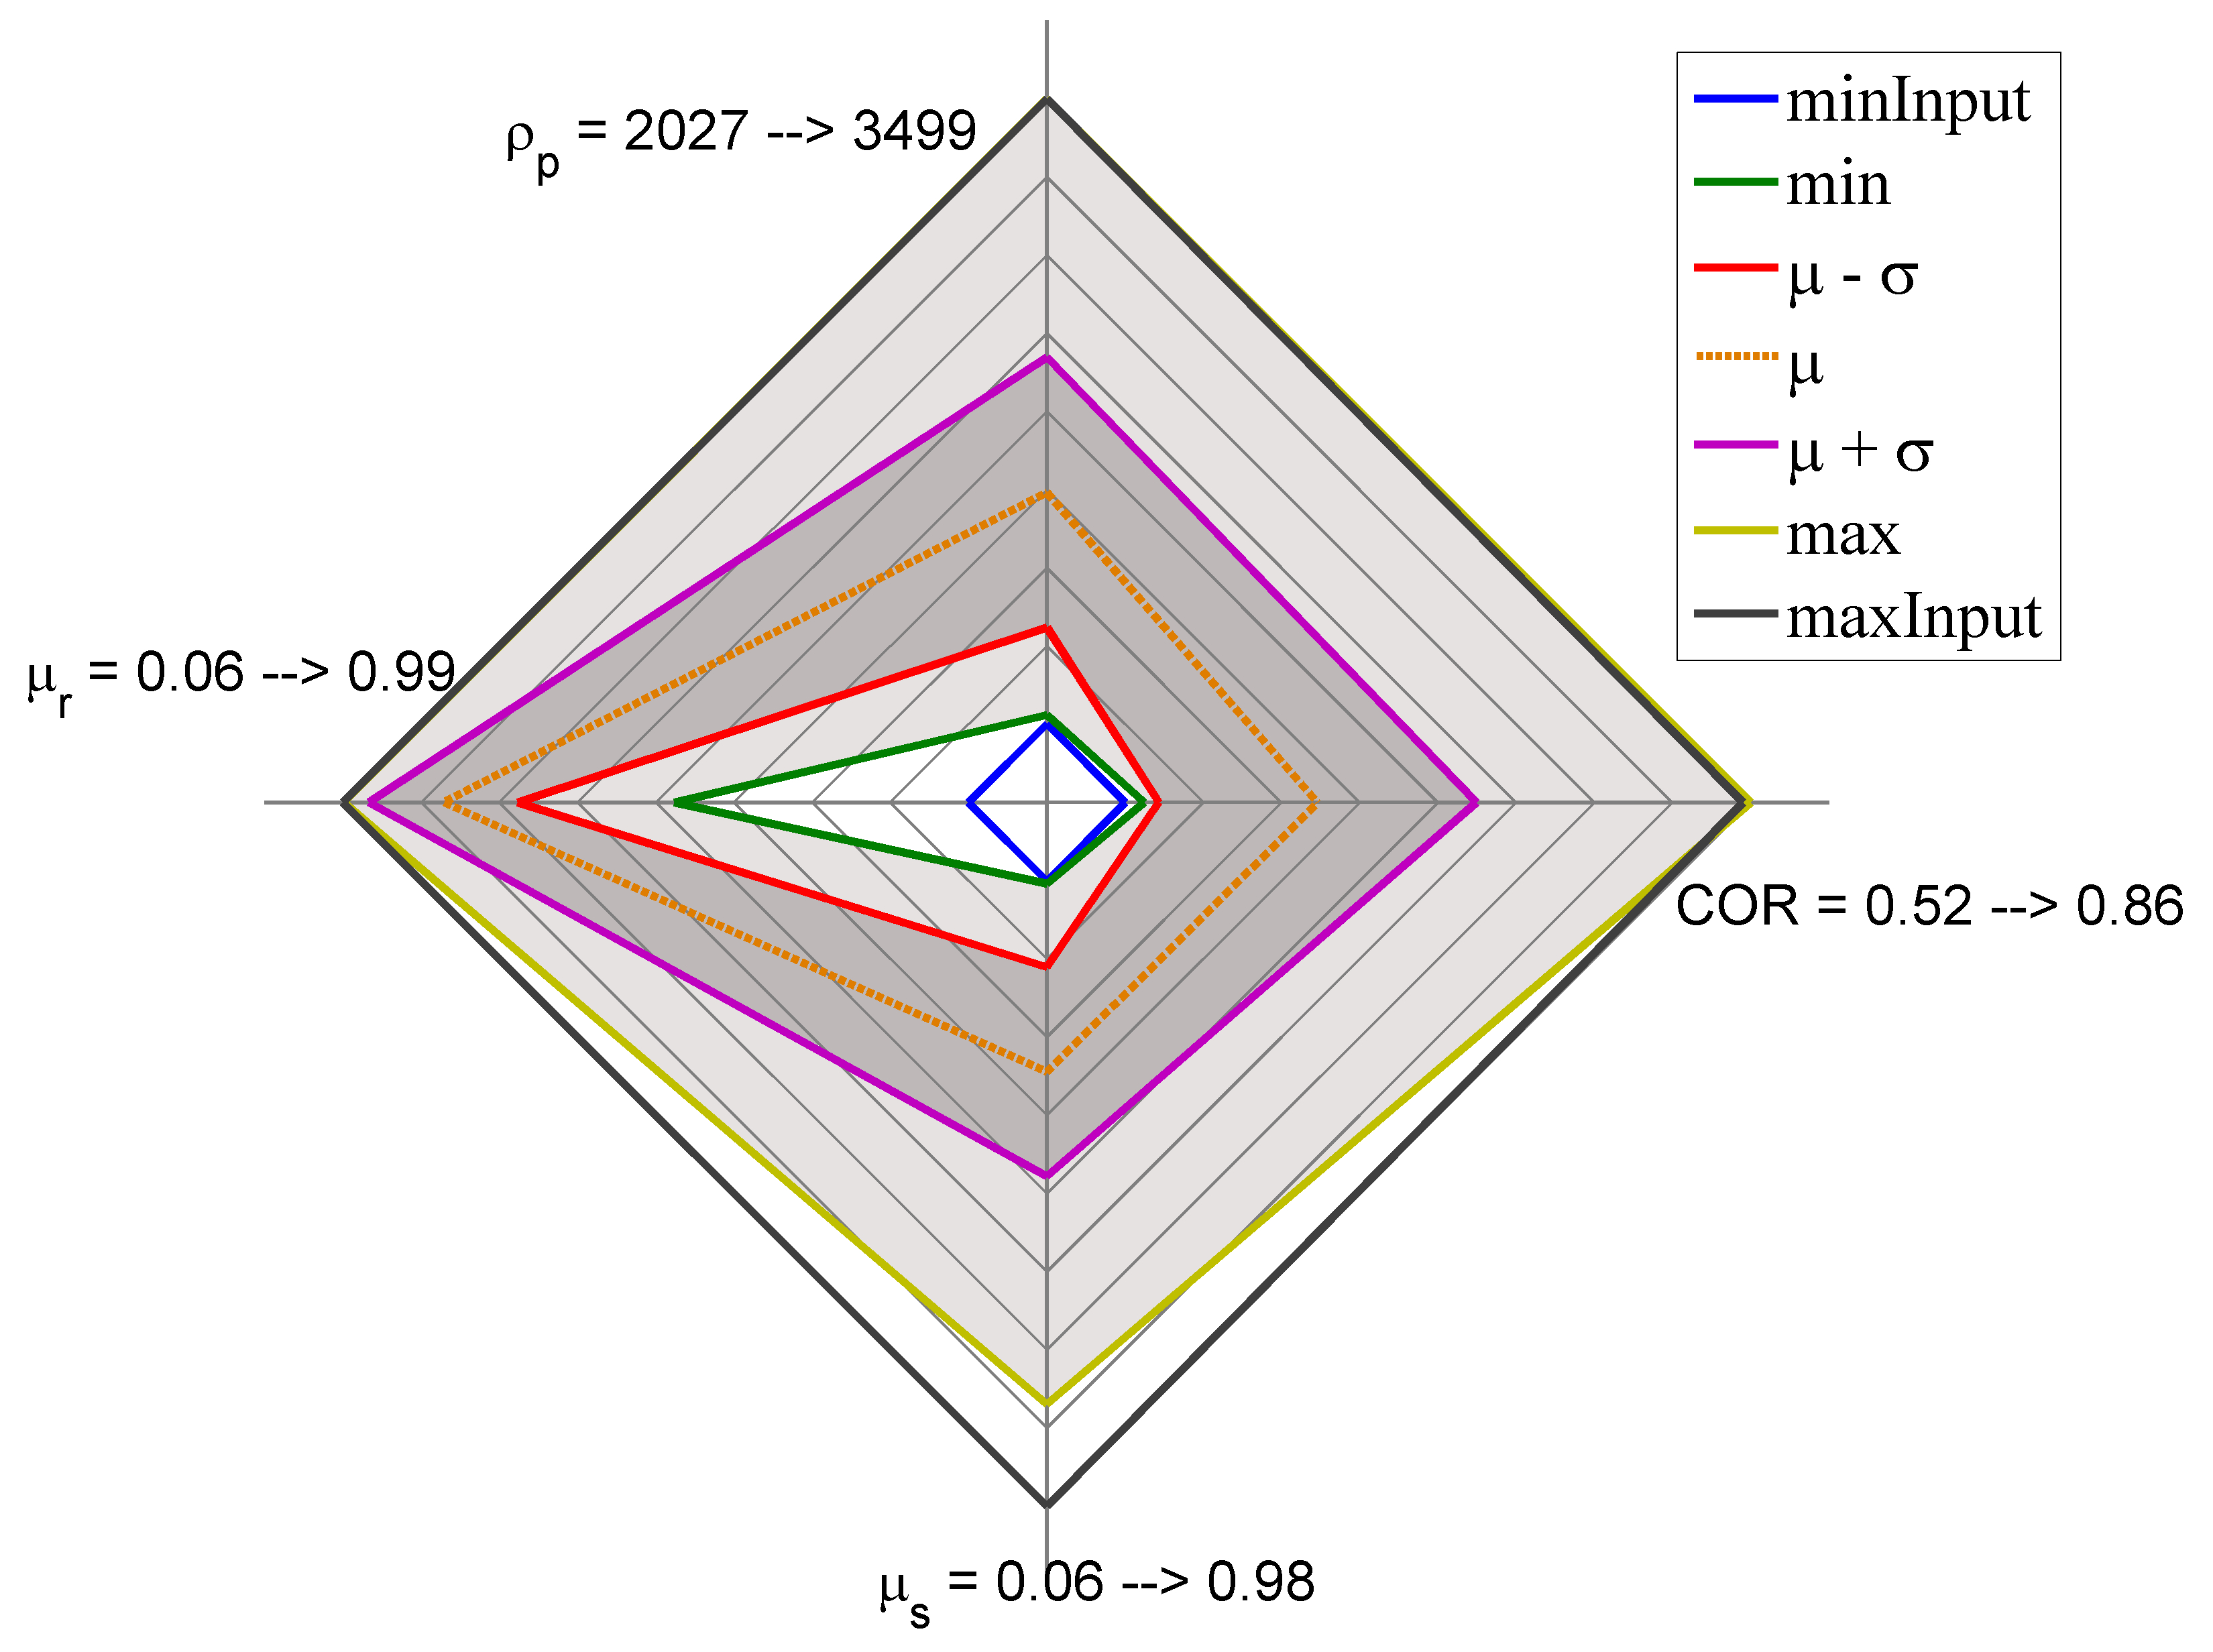
\includegraphics[width=\textwidth]{images/original/31radarpirker1aor}
        \caption{Radar P1 AOR}
        \label{fig:31radarpirker1aor} 
    \end{subfigure}
    \begin{subfigure}[b]{0.48\columnwidth}
        \includegraphics[width=\textwidth]{images/original/32cloudpirker1aor}
        \caption{Cloud P1 AOR}
        \label{fig:32cloudpirker1aor} 
    \end{subfigure}\\
        \begin{subfigure}[b]{0.48\columnwidth}
        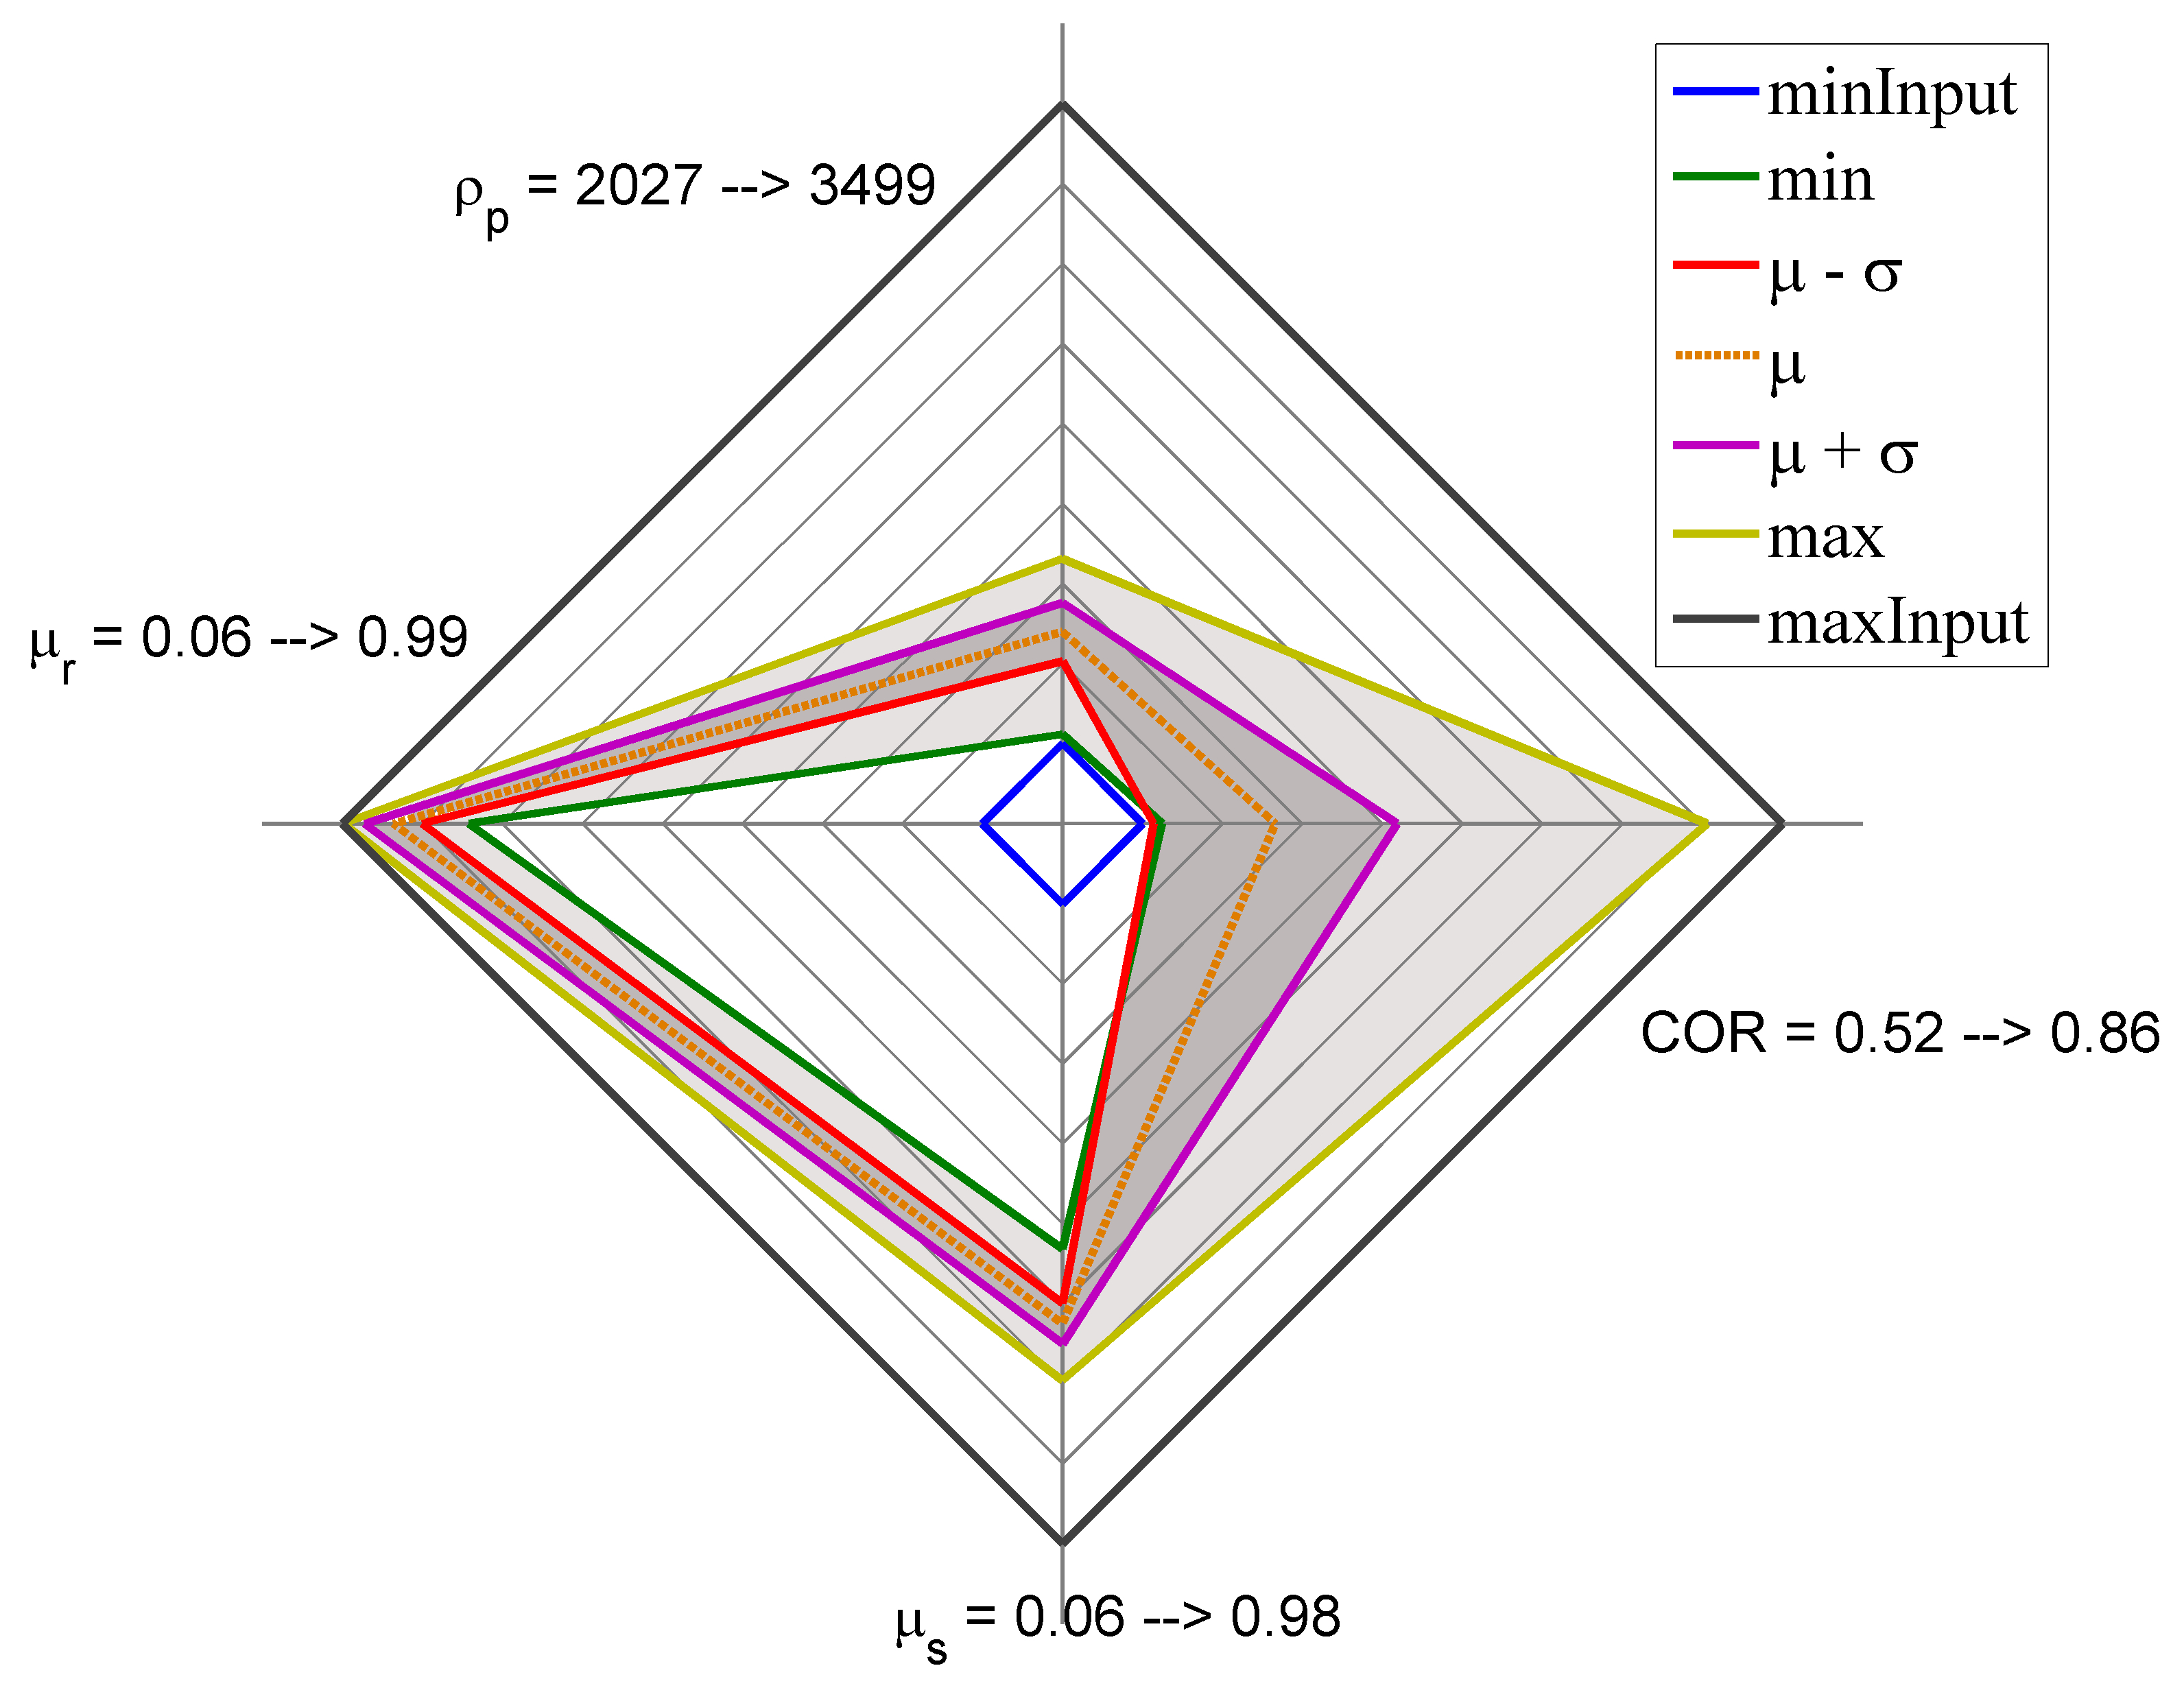
\includegraphics[width=\textwidth]{images/original/33radarpirker1schulze10070aor}
        \caption{Radar P1 Schulze 10070 & AOR}
        \label{fig:33radarpirker1schulze10070aor} 
    \end{subfigure}
    \begin{subfigure}[b]{0.48\columnwidth}
        \includegraphics[width=\textwidth]{images/original/34cloudpirker1schulze10070aor}
        \caption{Cloud P1 Schulze 10070 & AOR}
        \label{fig:34cloudpirker1schulze10070aor} 
    \end{subfigure}
    \caption{AOR and merge results.}
    \label{fig:35schulze10070aorradarandcloud}
\end{figure}
We then processed the random combinations with the $AOR$ $NN$. In Fig.
\ref{fig:31radarpirker1aor} the radar plot can be seen. In accordance with the
theory (Wensrich and Katterfeld \cite{RefWorks:87}), in a simulation dominated
by the particles rolling the coefficient of rolling friction has the maximum influence. 
Further, in the cloud plot in Fig. \ref{fig:32cloudpirker1aor}
we could see that there are valid combinations also with slight $\mu_s$. \\
Finally, we extracted from the tabbed combinations values ($P=1.0$) the $AOR$ $NN$ behaviour and compared it with the experimental one. 
As can be seen in the radar plot in Fig.
\ref{fig:33radarpirker1schulze10070aor}, the confidence range is meager, indicating that all the parameters but the $COR$ 
had an important role and the reliability of these parameters combinations to represent the bulk behaviour. 
Also in the cloud plot in Fig. \ref{fig:34cloudpirker1schulze10070aor} we
observed a condensed distribution of valid parameters.
From the initial 6250000 combinations, only 3884 of them are valid (0.0621 \%).
\begin{figure}%[!h] 
\centering 
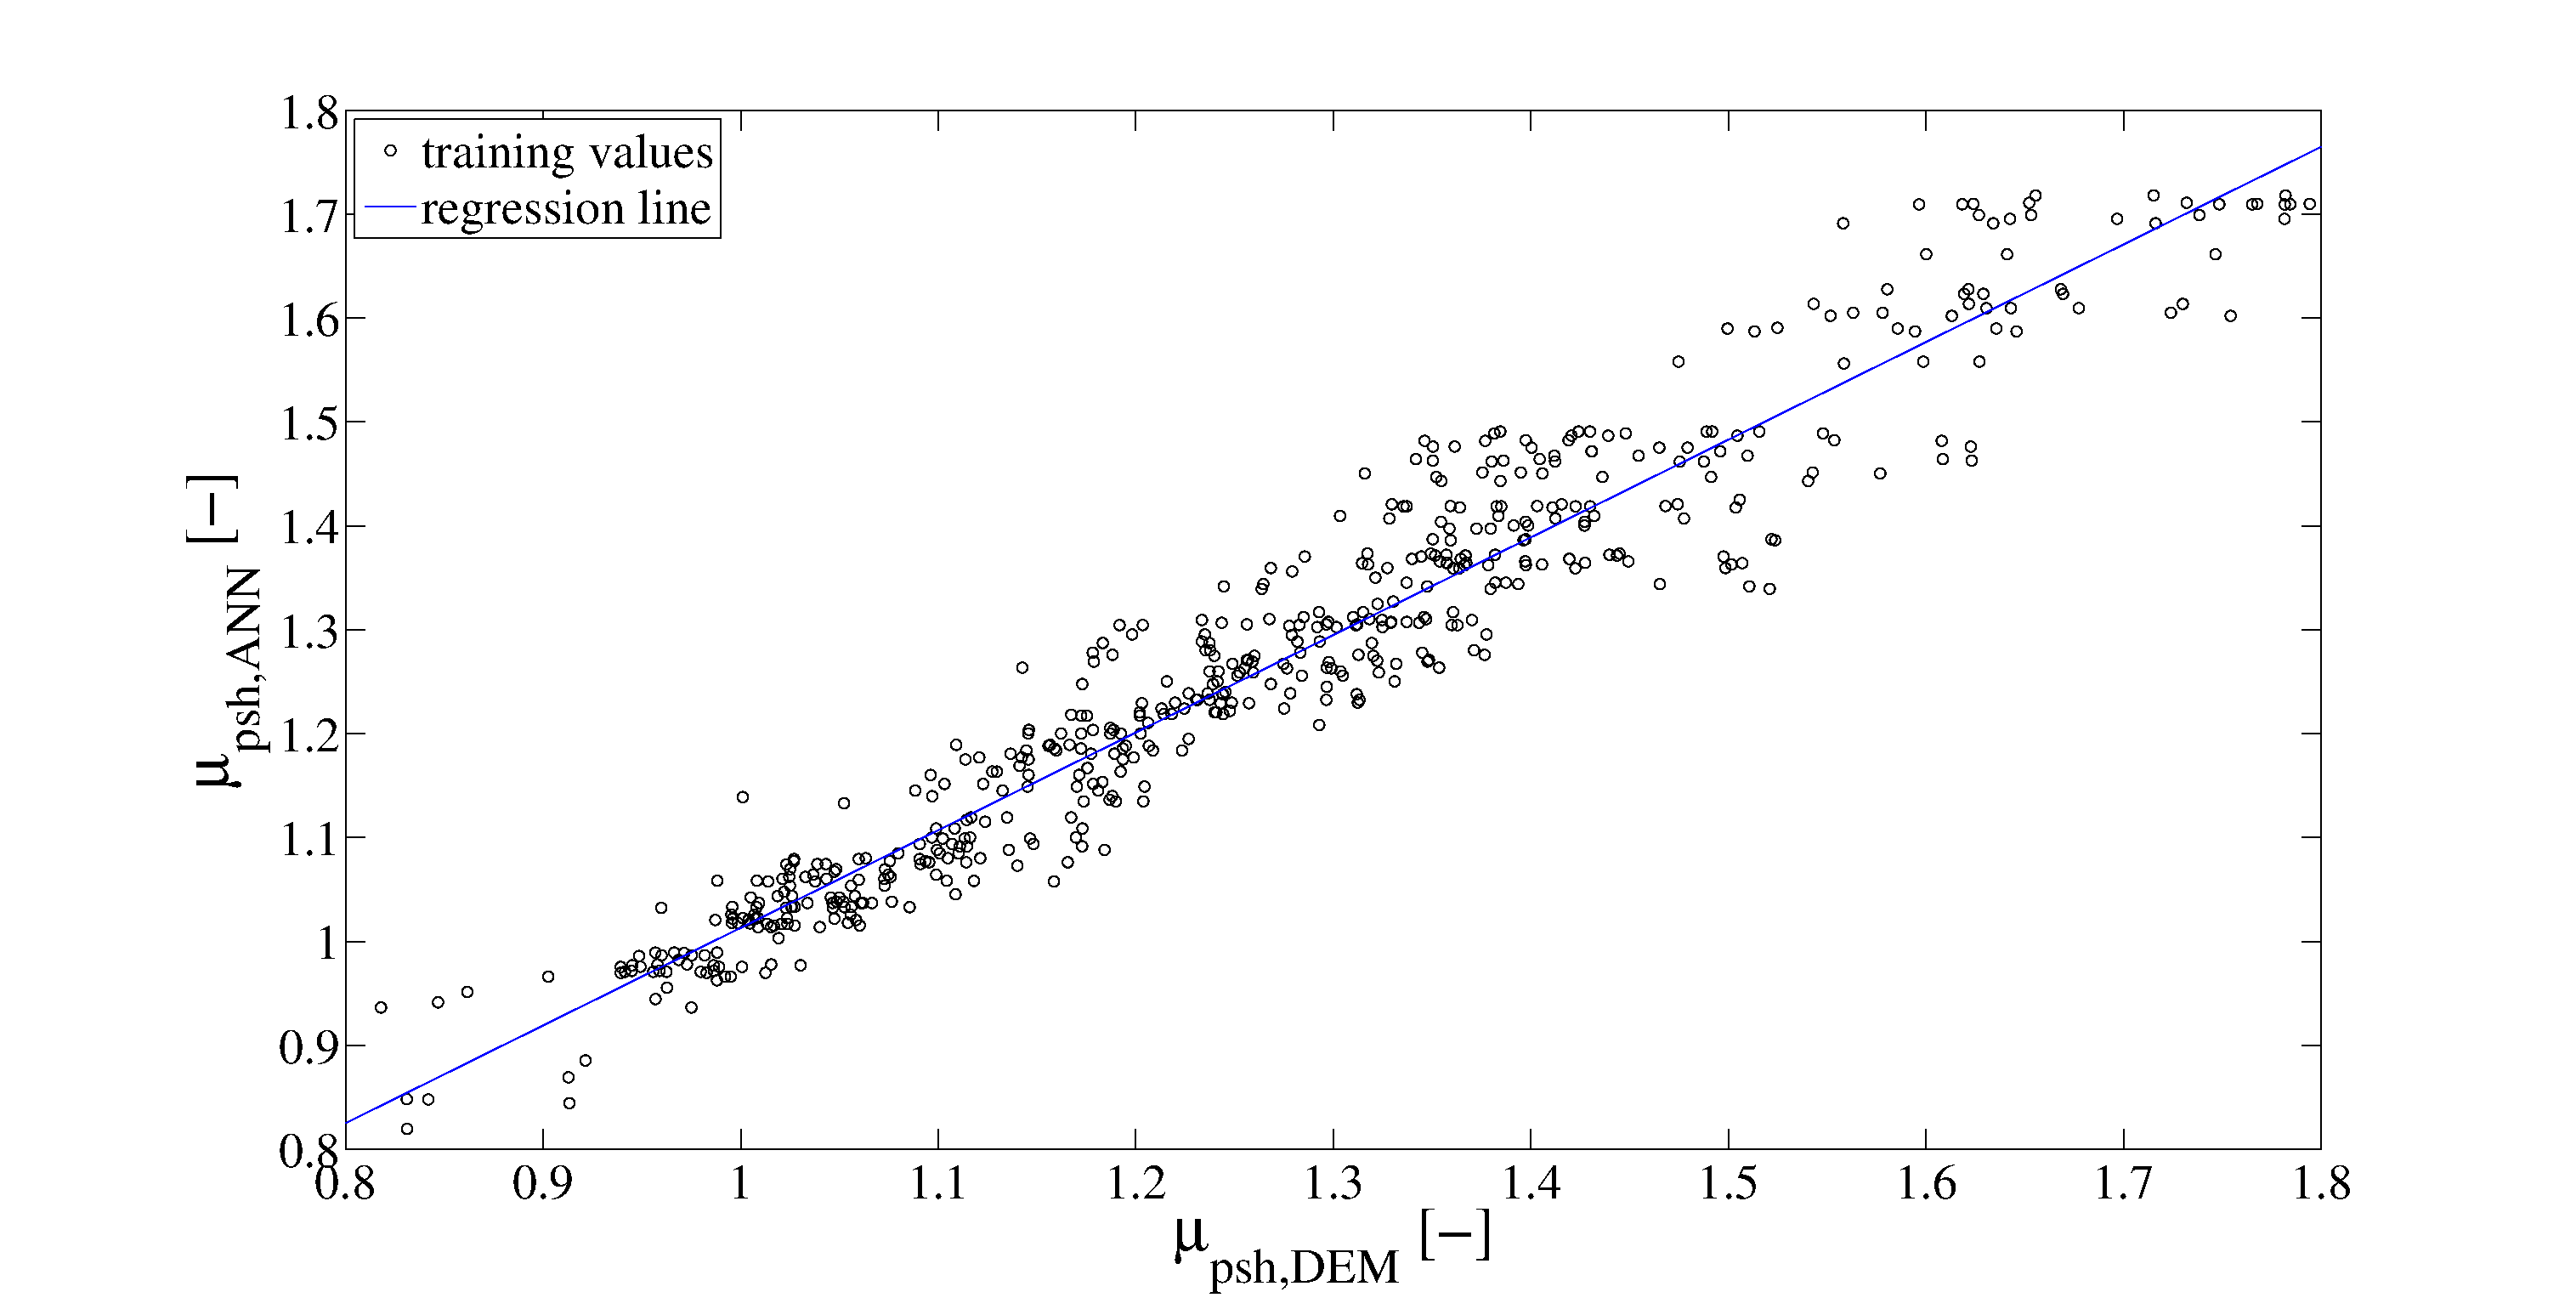
\includegraphics[width=.96\columnwidth]{images/22regression.eps}
%[width=.96\textwidth]
\caption[Comparison between prediction of the trained ANN and full DEM
simulation]{Comparison between prediction of the trained Artificial Neural
Network ($ANN$) and 546 
\wrong{write down all the simulations performed at the end.}
full DEM simulations of the coefficient of pre-shear
($\mu_{psh}$).}
\label{fig:22regression} 
\end{figure}
\begin{table}[h]
\centering
\scalebox{1.0}{
\begin{tabular}{c|cccccccc}
\hline
          & $\mu_s$ & $\mu_r$ & $COR$ & $\rho_p$ & $\mu_{sh}$ & $\mu_{psh}$ & $\rho_{b}$ & $AOR$ \\
          \hline
    $\mu_s$ & 100.00 & 0.55  & 0.04  & 0.00  & 3.84  & 87.26 & 8.39  & 49.48 \\
    $\mu_r$ & 0.55  & 100.00 & 0.15  & 0.00  & 58.92 & 33.70 & 3.10  & 60.20 \\
    $COR$ & 0.04  & 0.15  & 100.00 & 0.00  & 15.52 & 0.57  & 1.71  & 0.00 \\
    $\rho_p$ & 0.00  & 0.00  & 0.00  & 100.00 & 4.98  & 5.71  & 99.00 & 0.00 \\
    $\mu_{sh}$ & 3.84  & 58.92 & 15.52 & 4.98  & 100.00 & 26.03 & 9.52  & 0.00 \\
    $\mu_{psh}$ & \textbf{87.26} & 33.70 & 0.57  & 5.71  & 26.03 & 100.00 & 4.33 
    & 0.00
    \\
    $\rho_{b}$ & 8.39  & 3.10  & 1.71  & \textbf{99.00} & 9.52  & 4.33  & 100.00
    & 0.00 \\
    $AOR$ & 49.48 & \textbf{60.20} & 0.00  & 0.00  & 0.00  & 0.00  & 0.00  &
    100.00 \\
    
\hline
\end{tabular}}
\caption{Values of linear relationship between considered variables multiplied
for 100}
\label{tab:06inputRelationshipTable}
\end{table}
\begin{figure}[!h] 
\centering 
\includegraphics[width=.96\textwidth]{images/original/23regressiongraph}
%[width=.96\textwidth]
\caption{Regression graph}
\label{fig:23regressiongraph} 
\end{figure}


% \begin{figure}[htp]
%     \centering
%     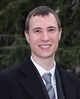
\includegraphics[width=.2\textwidth]{images/vitae/lbenvenuti}
%     \caption{OpenMP, MPI, MPI/OpenMP Hybrid runs of Box in a box testcase on 32
%     cores. The OpenMP-only run suffers from limited memory bandwidth in
%     memory-bound algorithms inside of the Modify section of the code. MPI-only has
%     low averaged runtimes for each section, but a very large Other timing, which
%     hints for a large amount of load-imbalance. Hybrid timings are a bit worse
%     on average, but because of better balancing, processes have lower wait times
%     inside of Other timing.}
% 	\label{fig:boxInBoxComparison}

\begin{figure}[htp] \centering
    \begin{subfigure}[b]{0.48\columnwidth}
        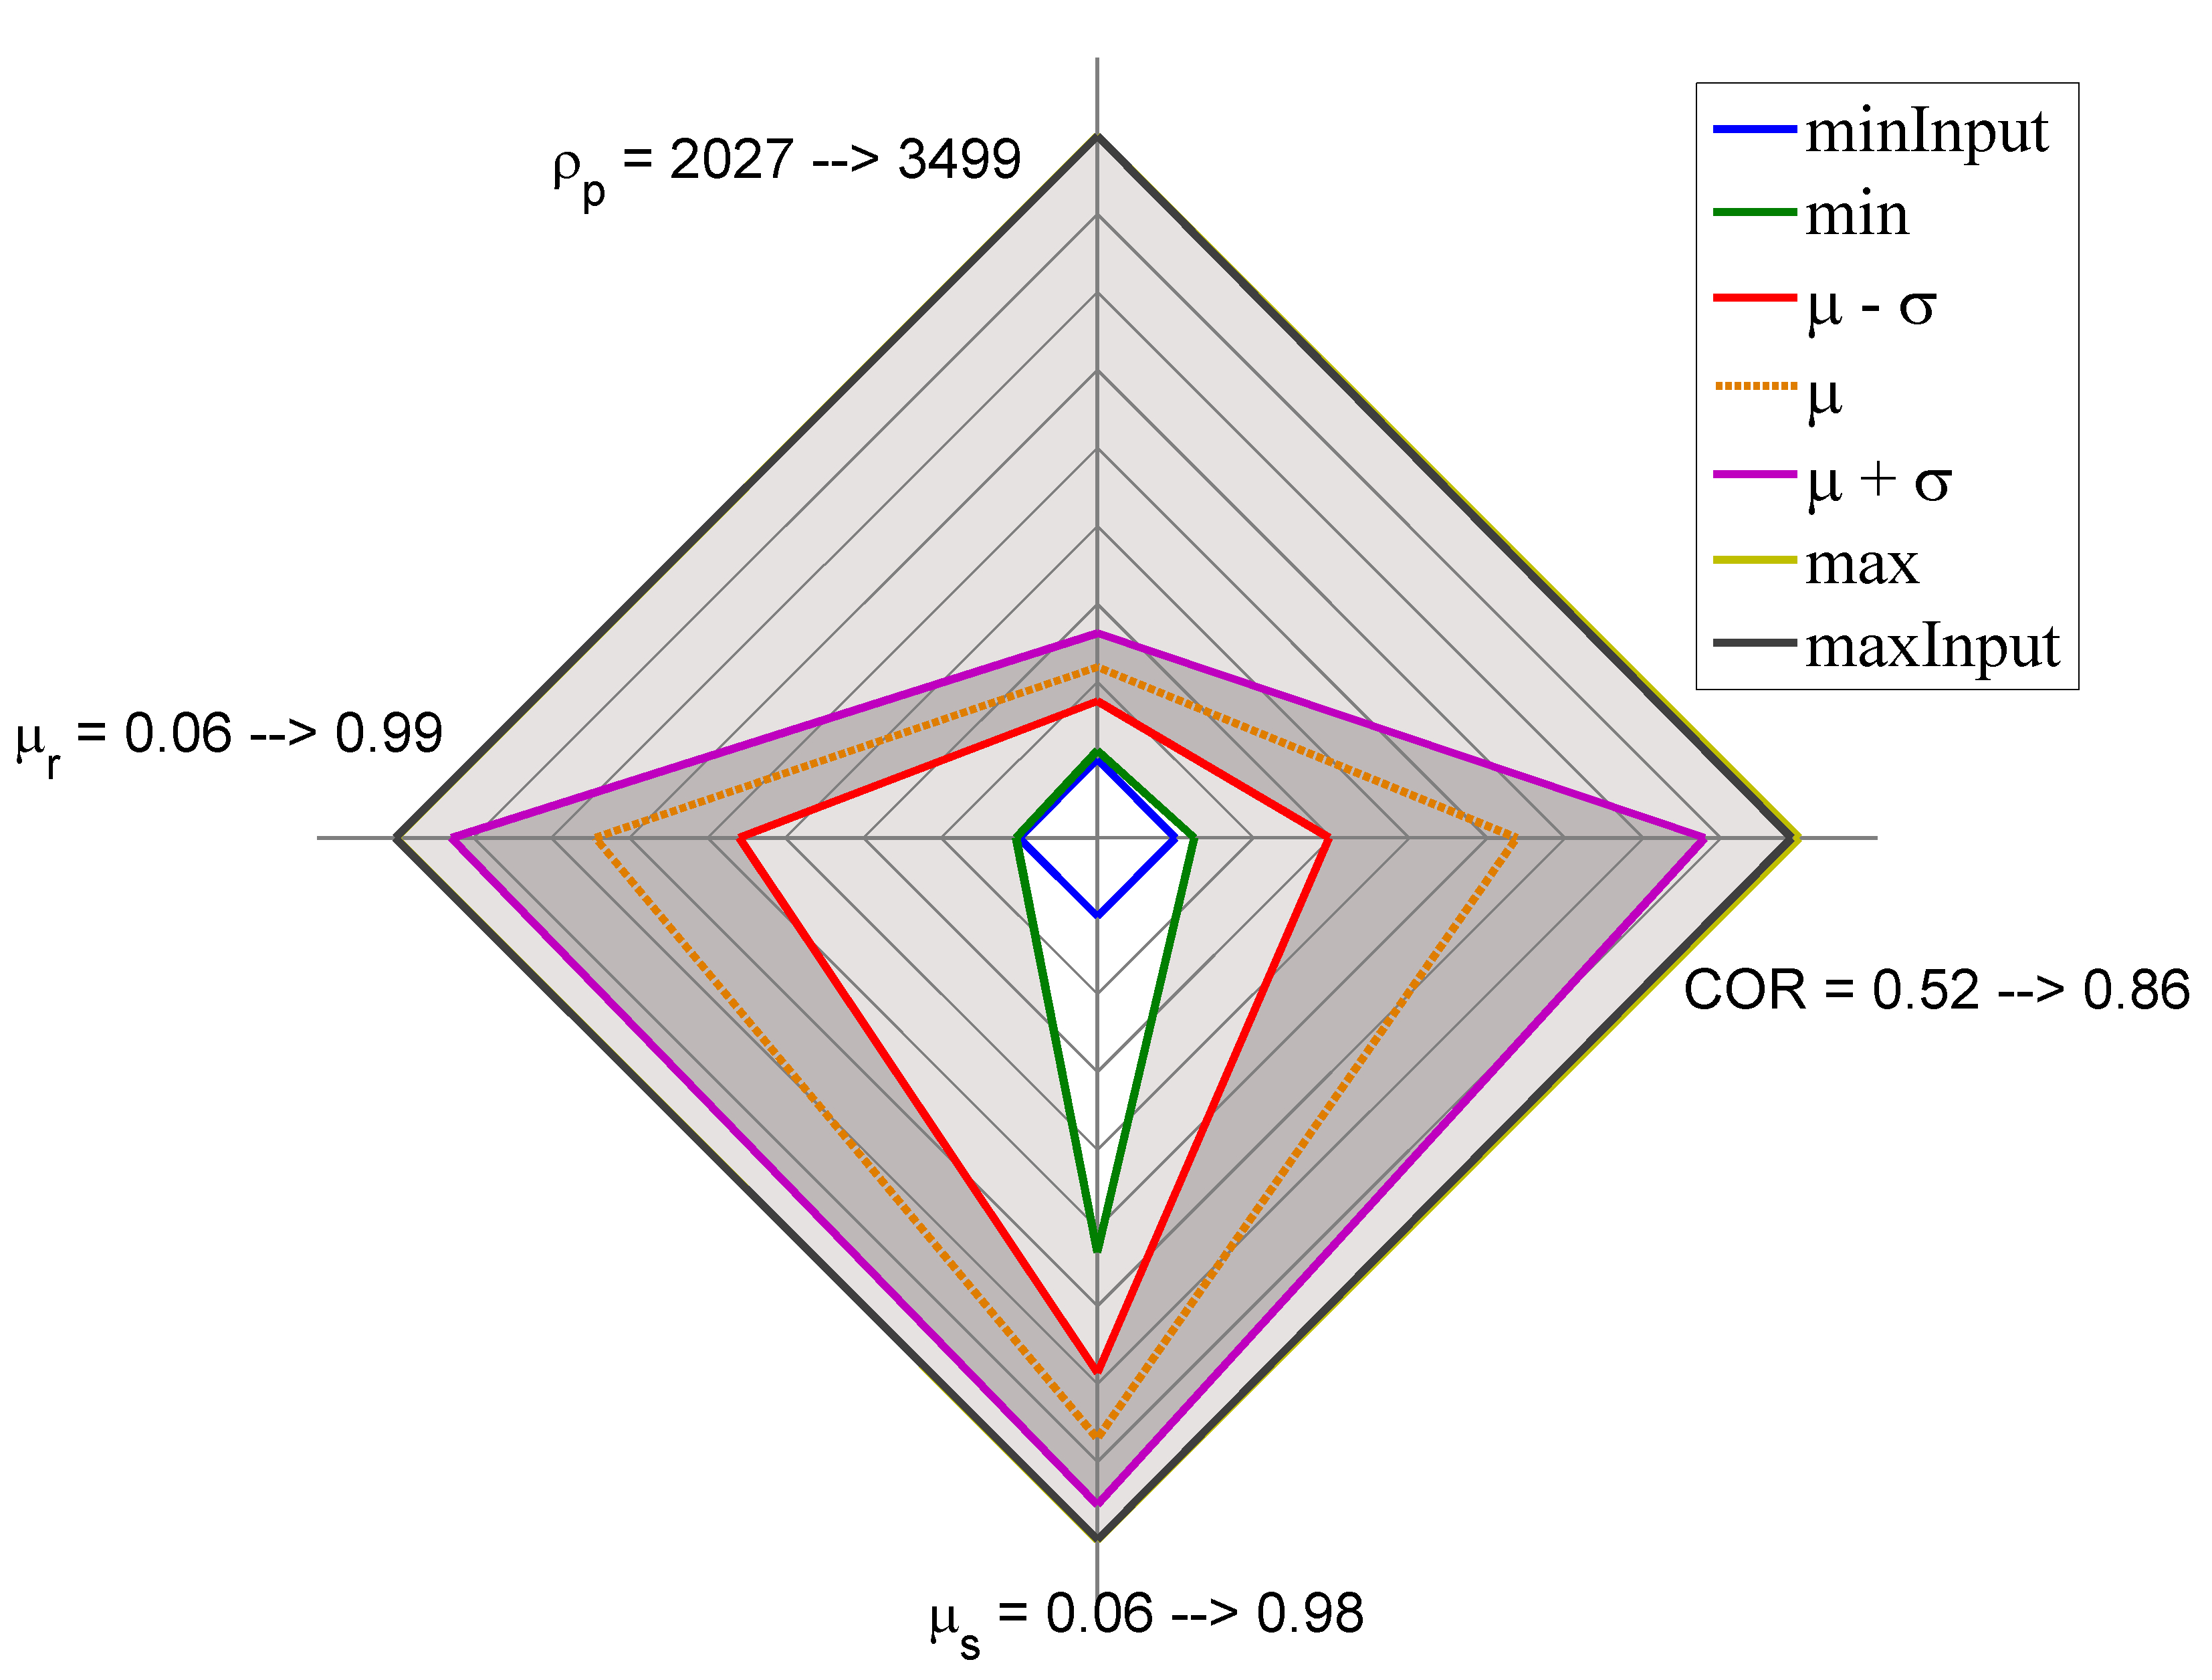
\includegraphics[width=\textwidth]{images/original/24radarpirker1schulze10070}
        \caption{Radar P1 Schulze10070}
        \label{fig:24radarpirker1schulze10070}
    \end{subfigure}
    \begin{subfigure}[b]{0.48\columnwidth}
        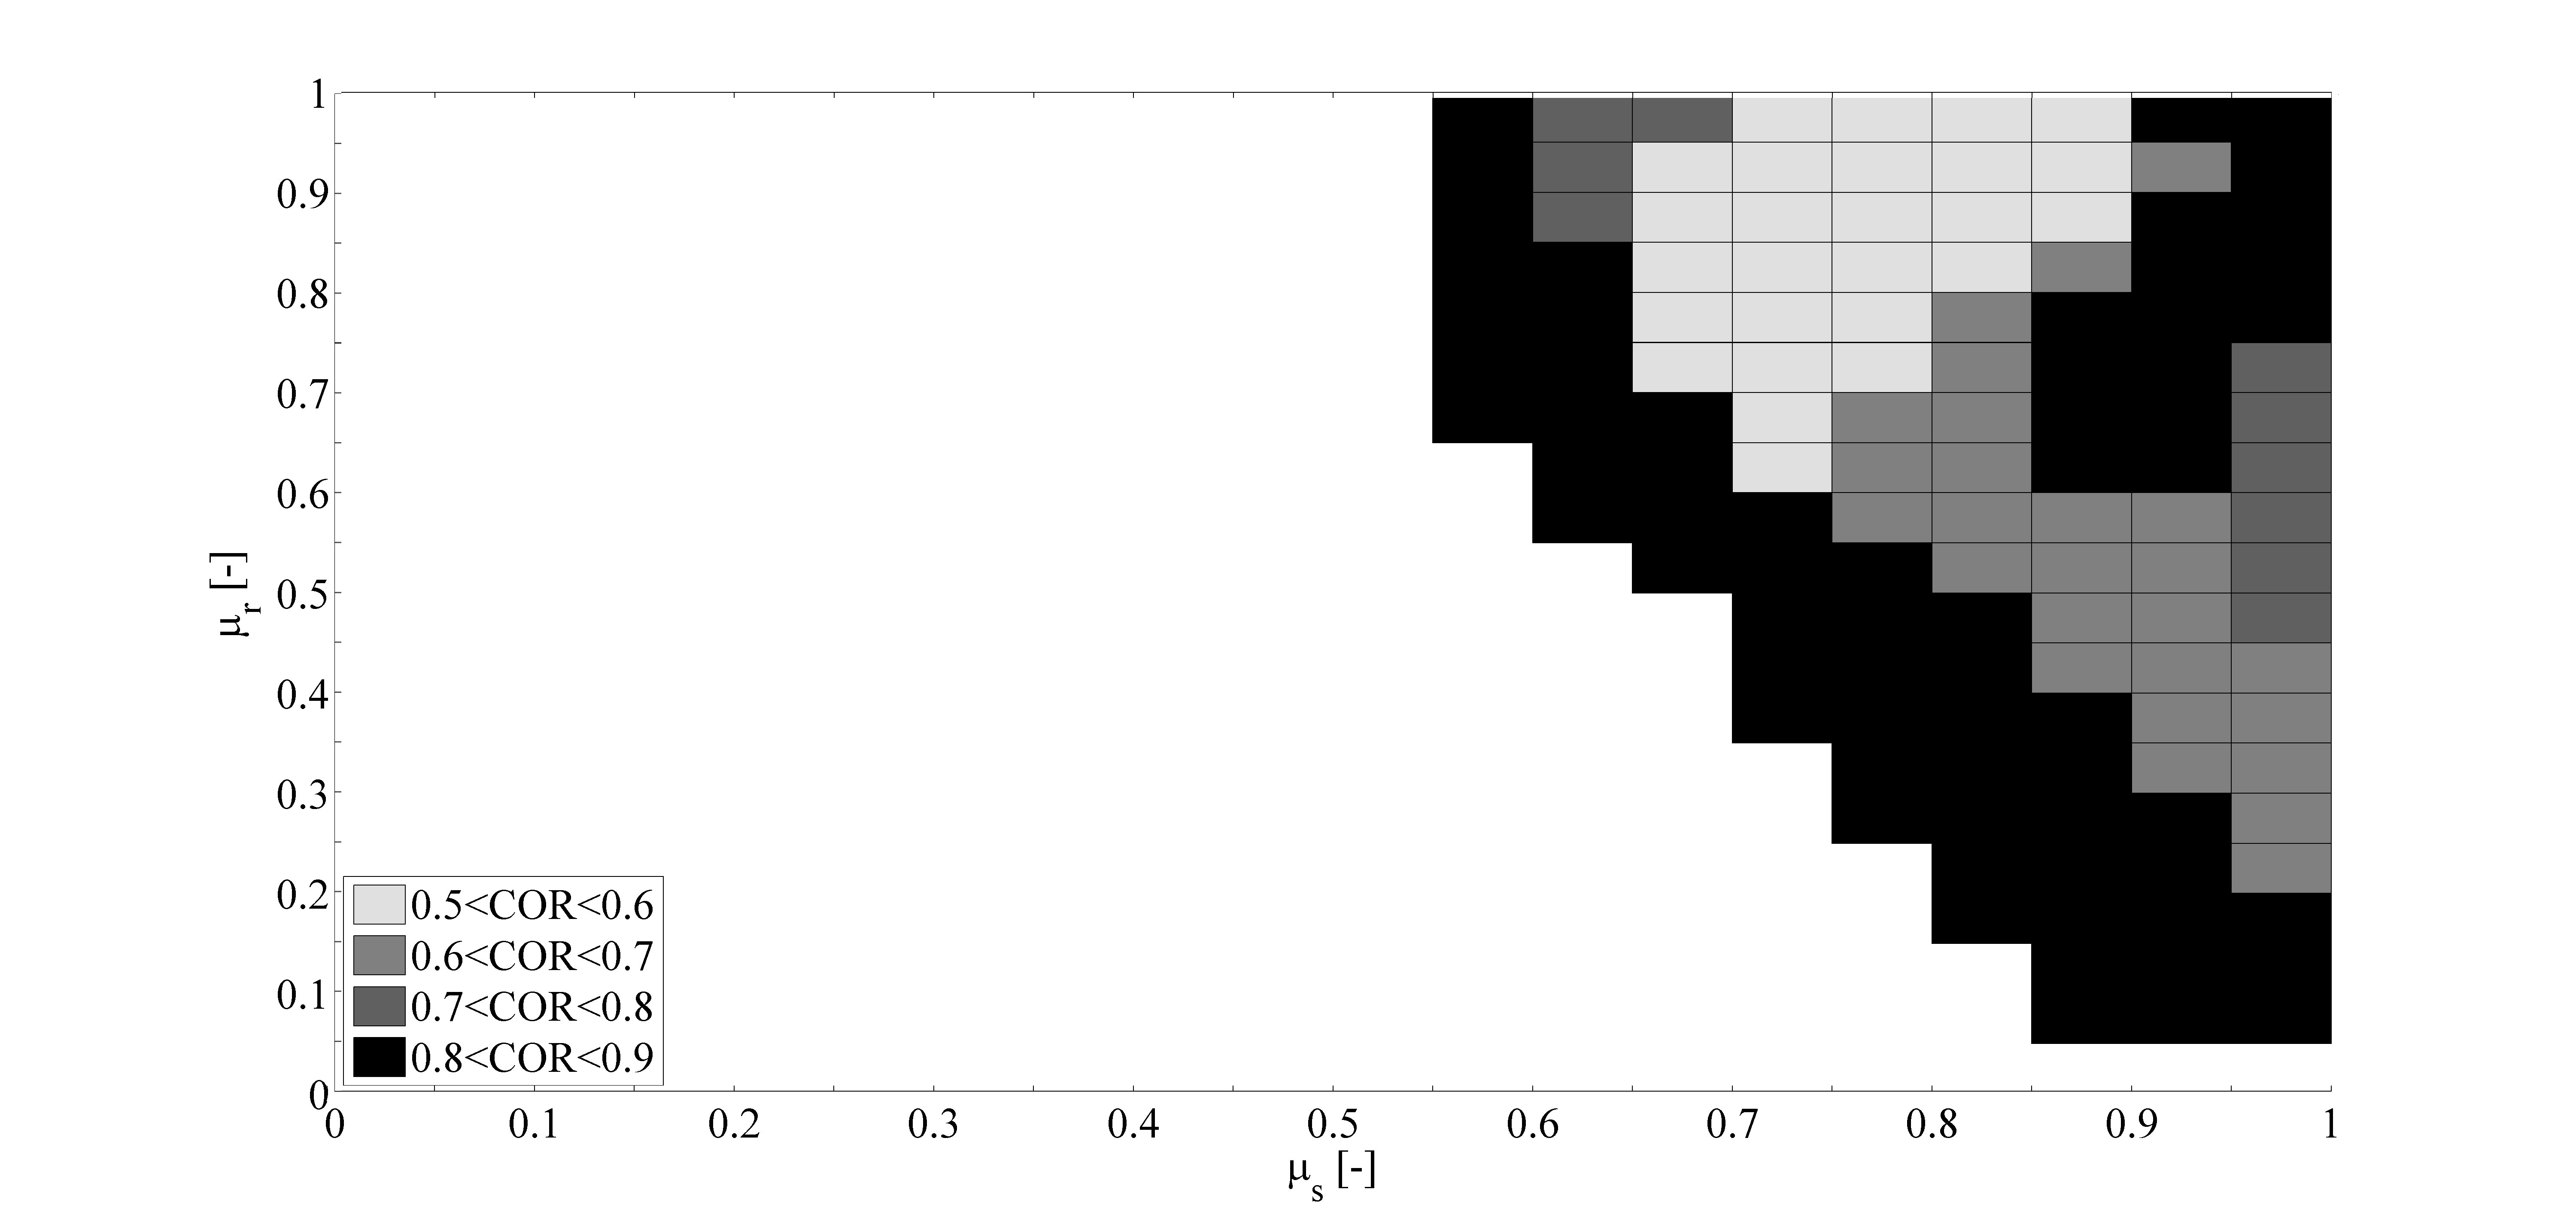
\includegraphics[width=\textwidth]{images/original/25cloudpirker1schulze10070}
        \caption{Cloud P1 Schulze10070}
        \label{fig:25cloudpirker1schulze10070}
    \end{subfigure}\\
        \begin{subfigure}[b]{0.48\columnwidth}
        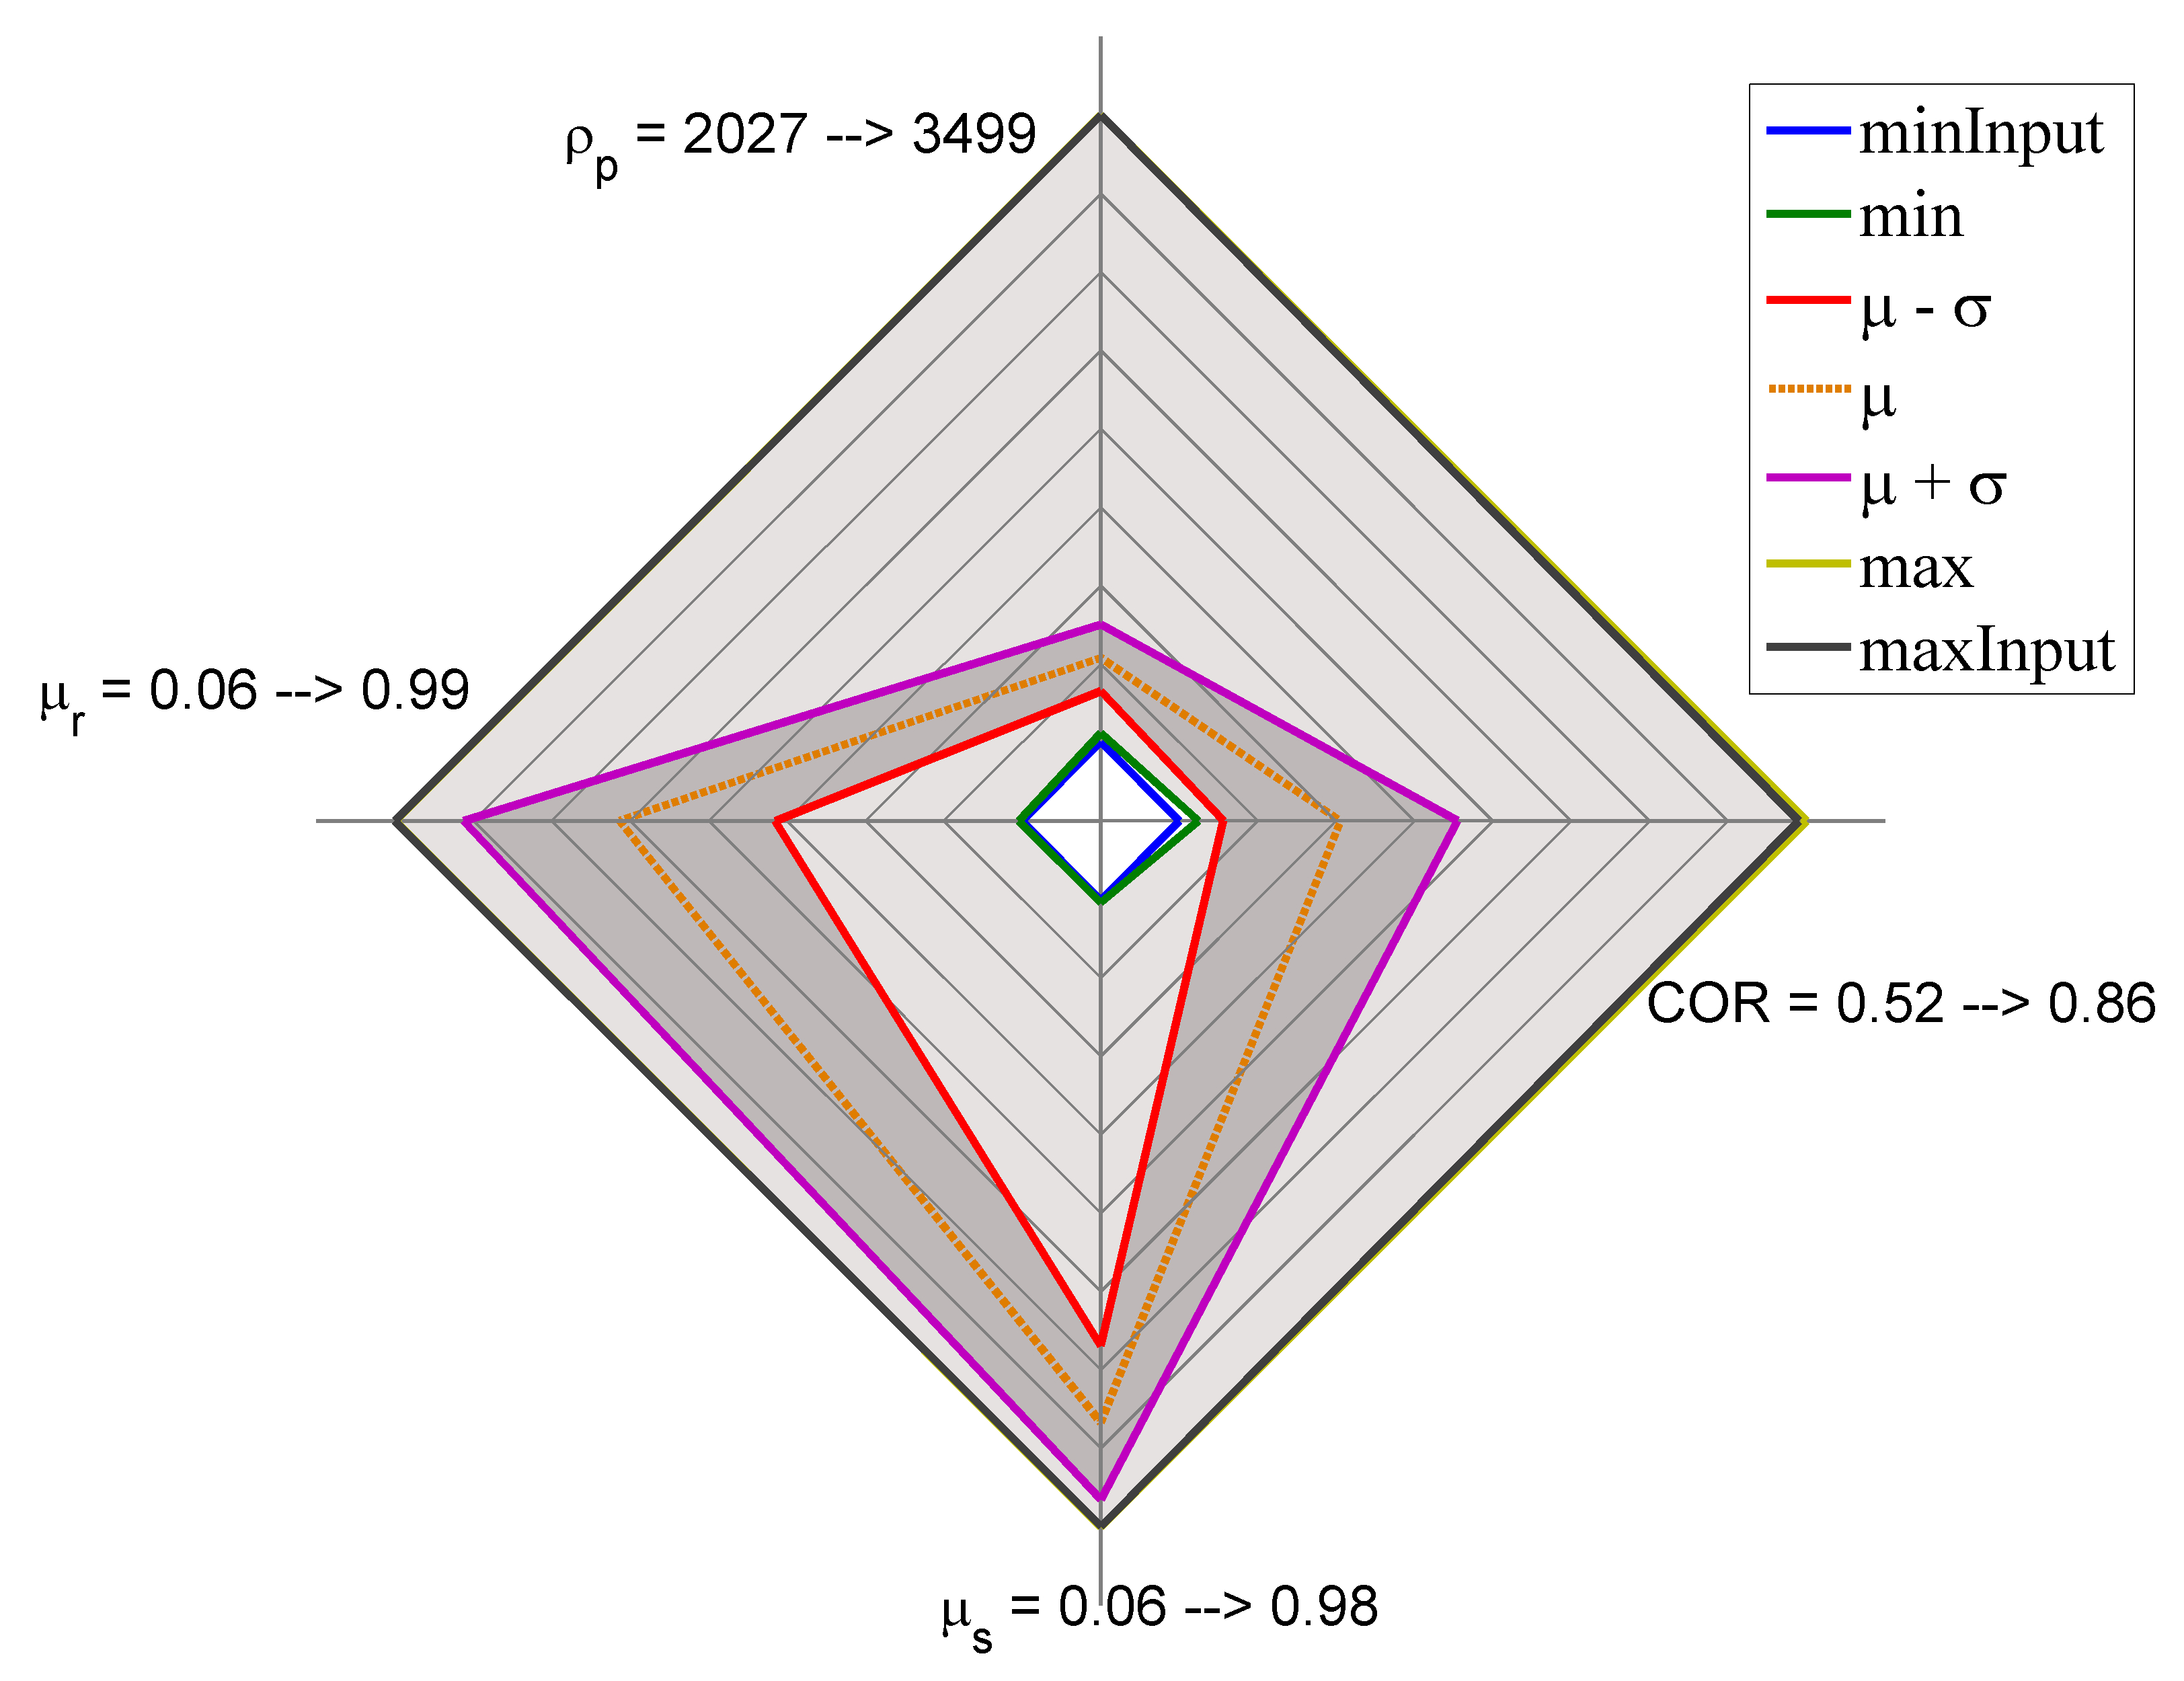
\includegraphics[width=\textwidth]{images/original/26radarpirker08schulze10070}
        \caption{Radar P08 Schulze10070}
        \label{fig:26radarpirker08schulze10070} 
    \end{subfigure}
    \begin{subfigure}[b]{0.48\columnwidth}
        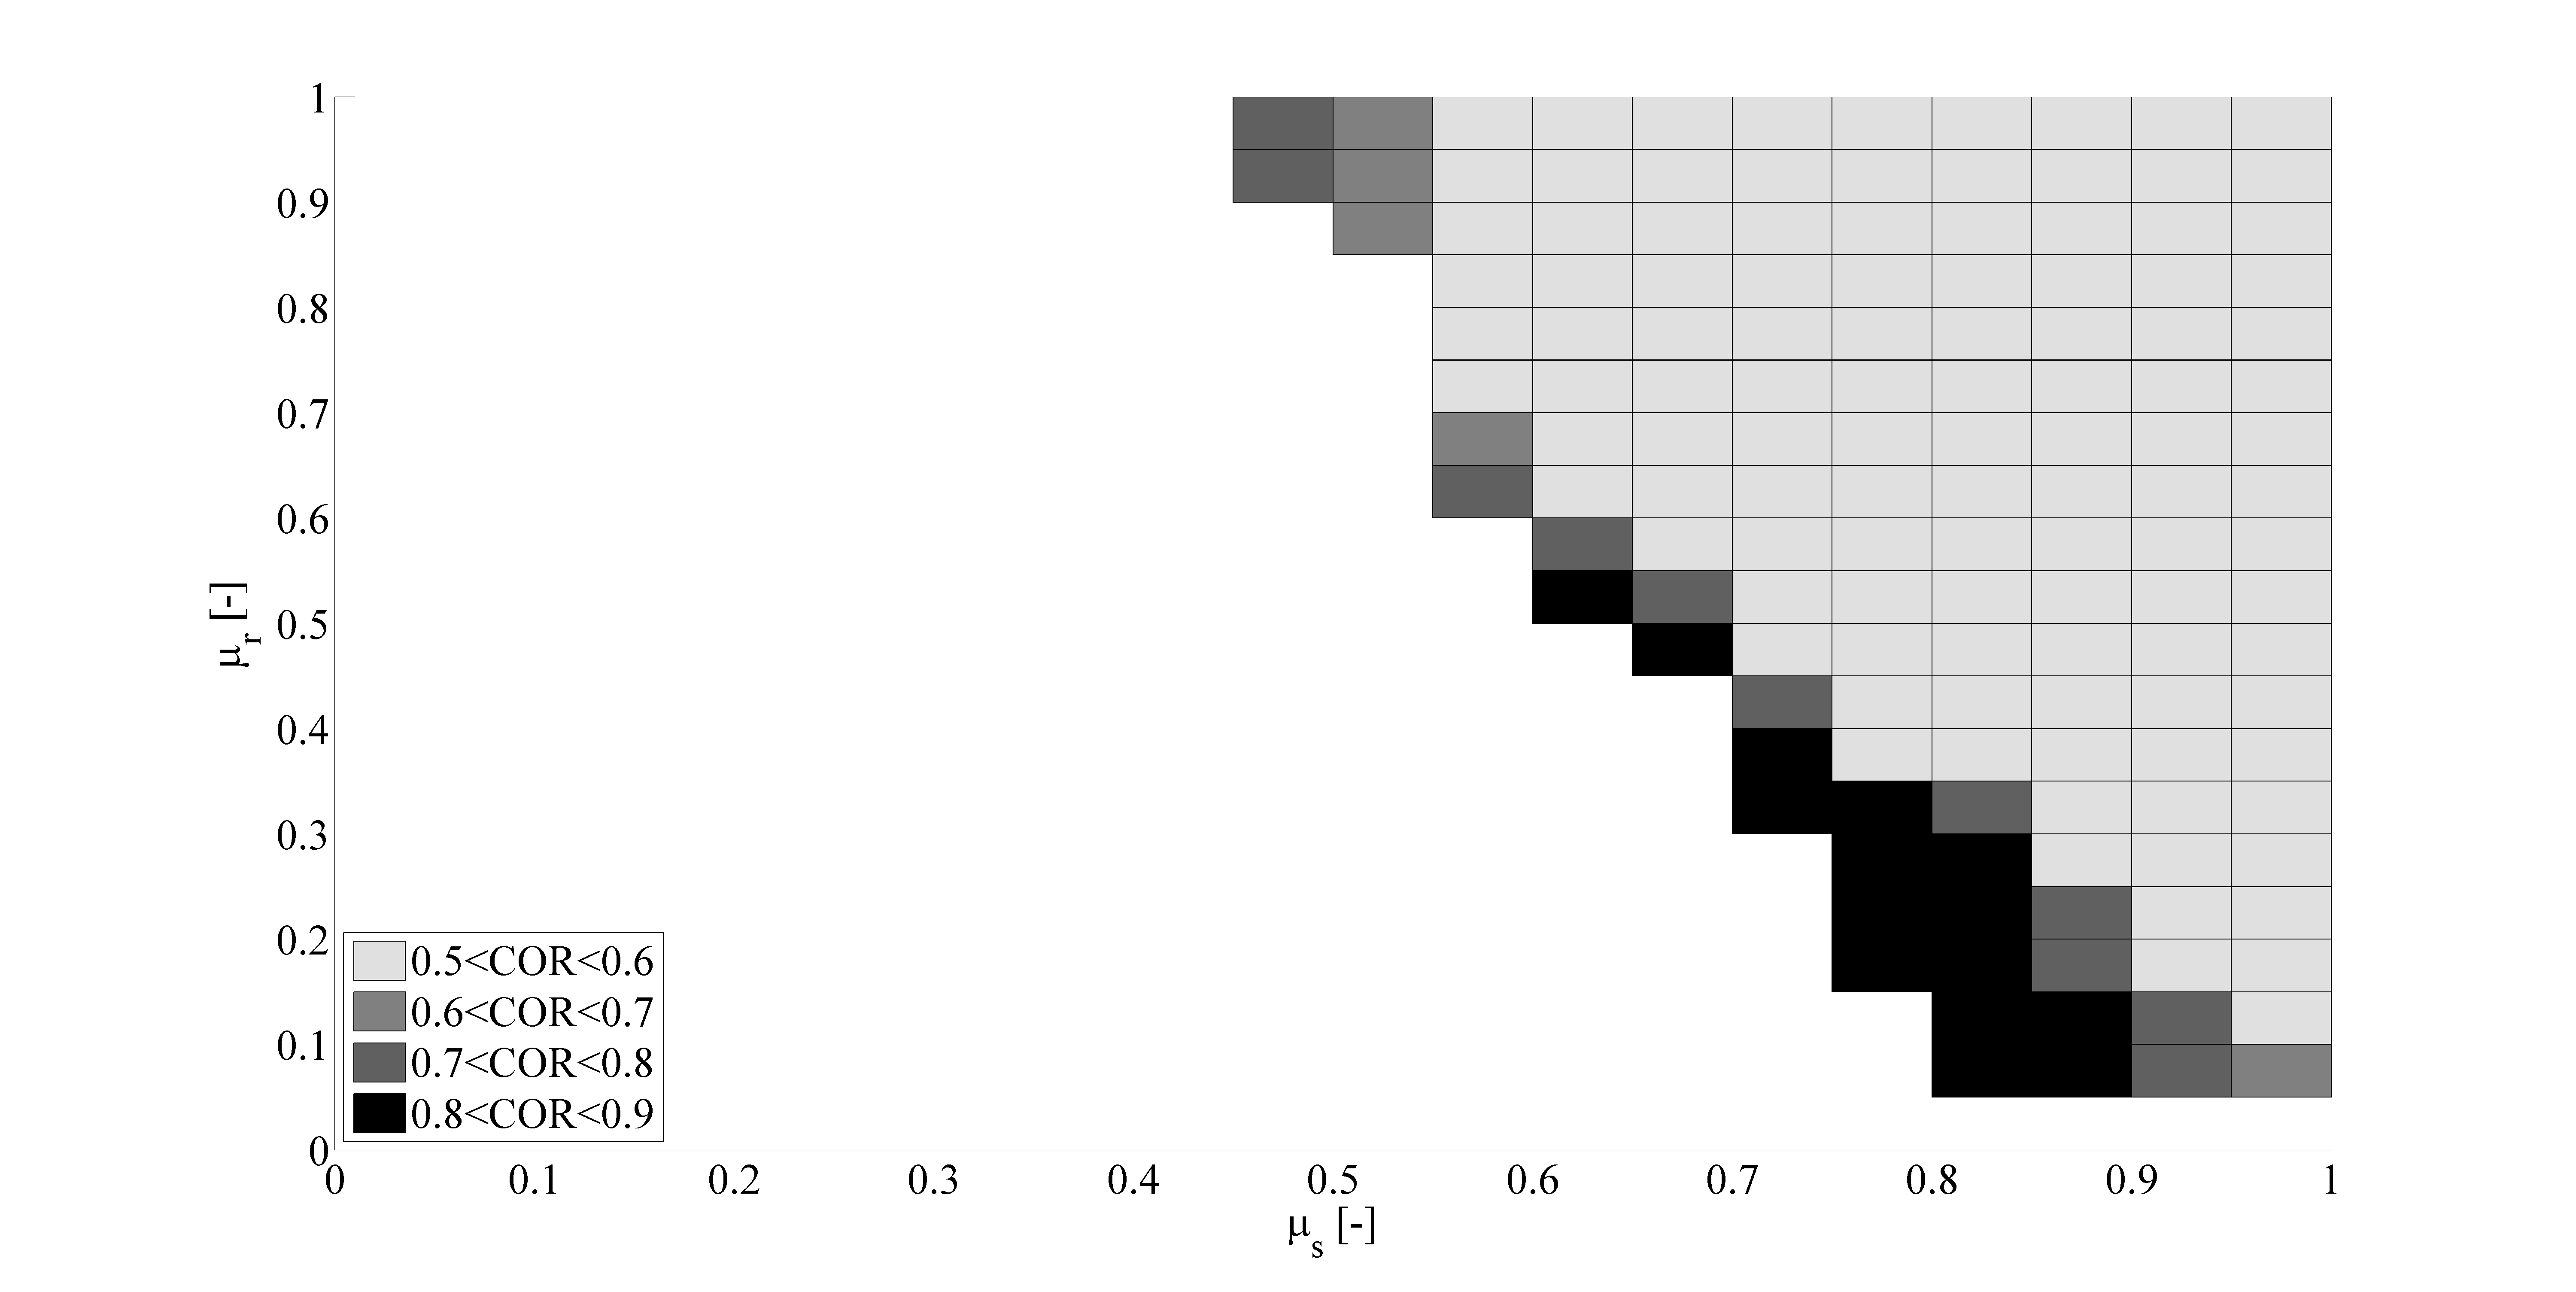
\includegraphics[width=\textwidth]{images/original/27cloudpirker08schulze10070}
        \caption{Cloud P08 Schulze10070}
        \label{fig:27cloudpirker08schulze10070} 
    \end{subfigure}\\
        \begin{subfigure}[b]{0.48\columnwidth}
        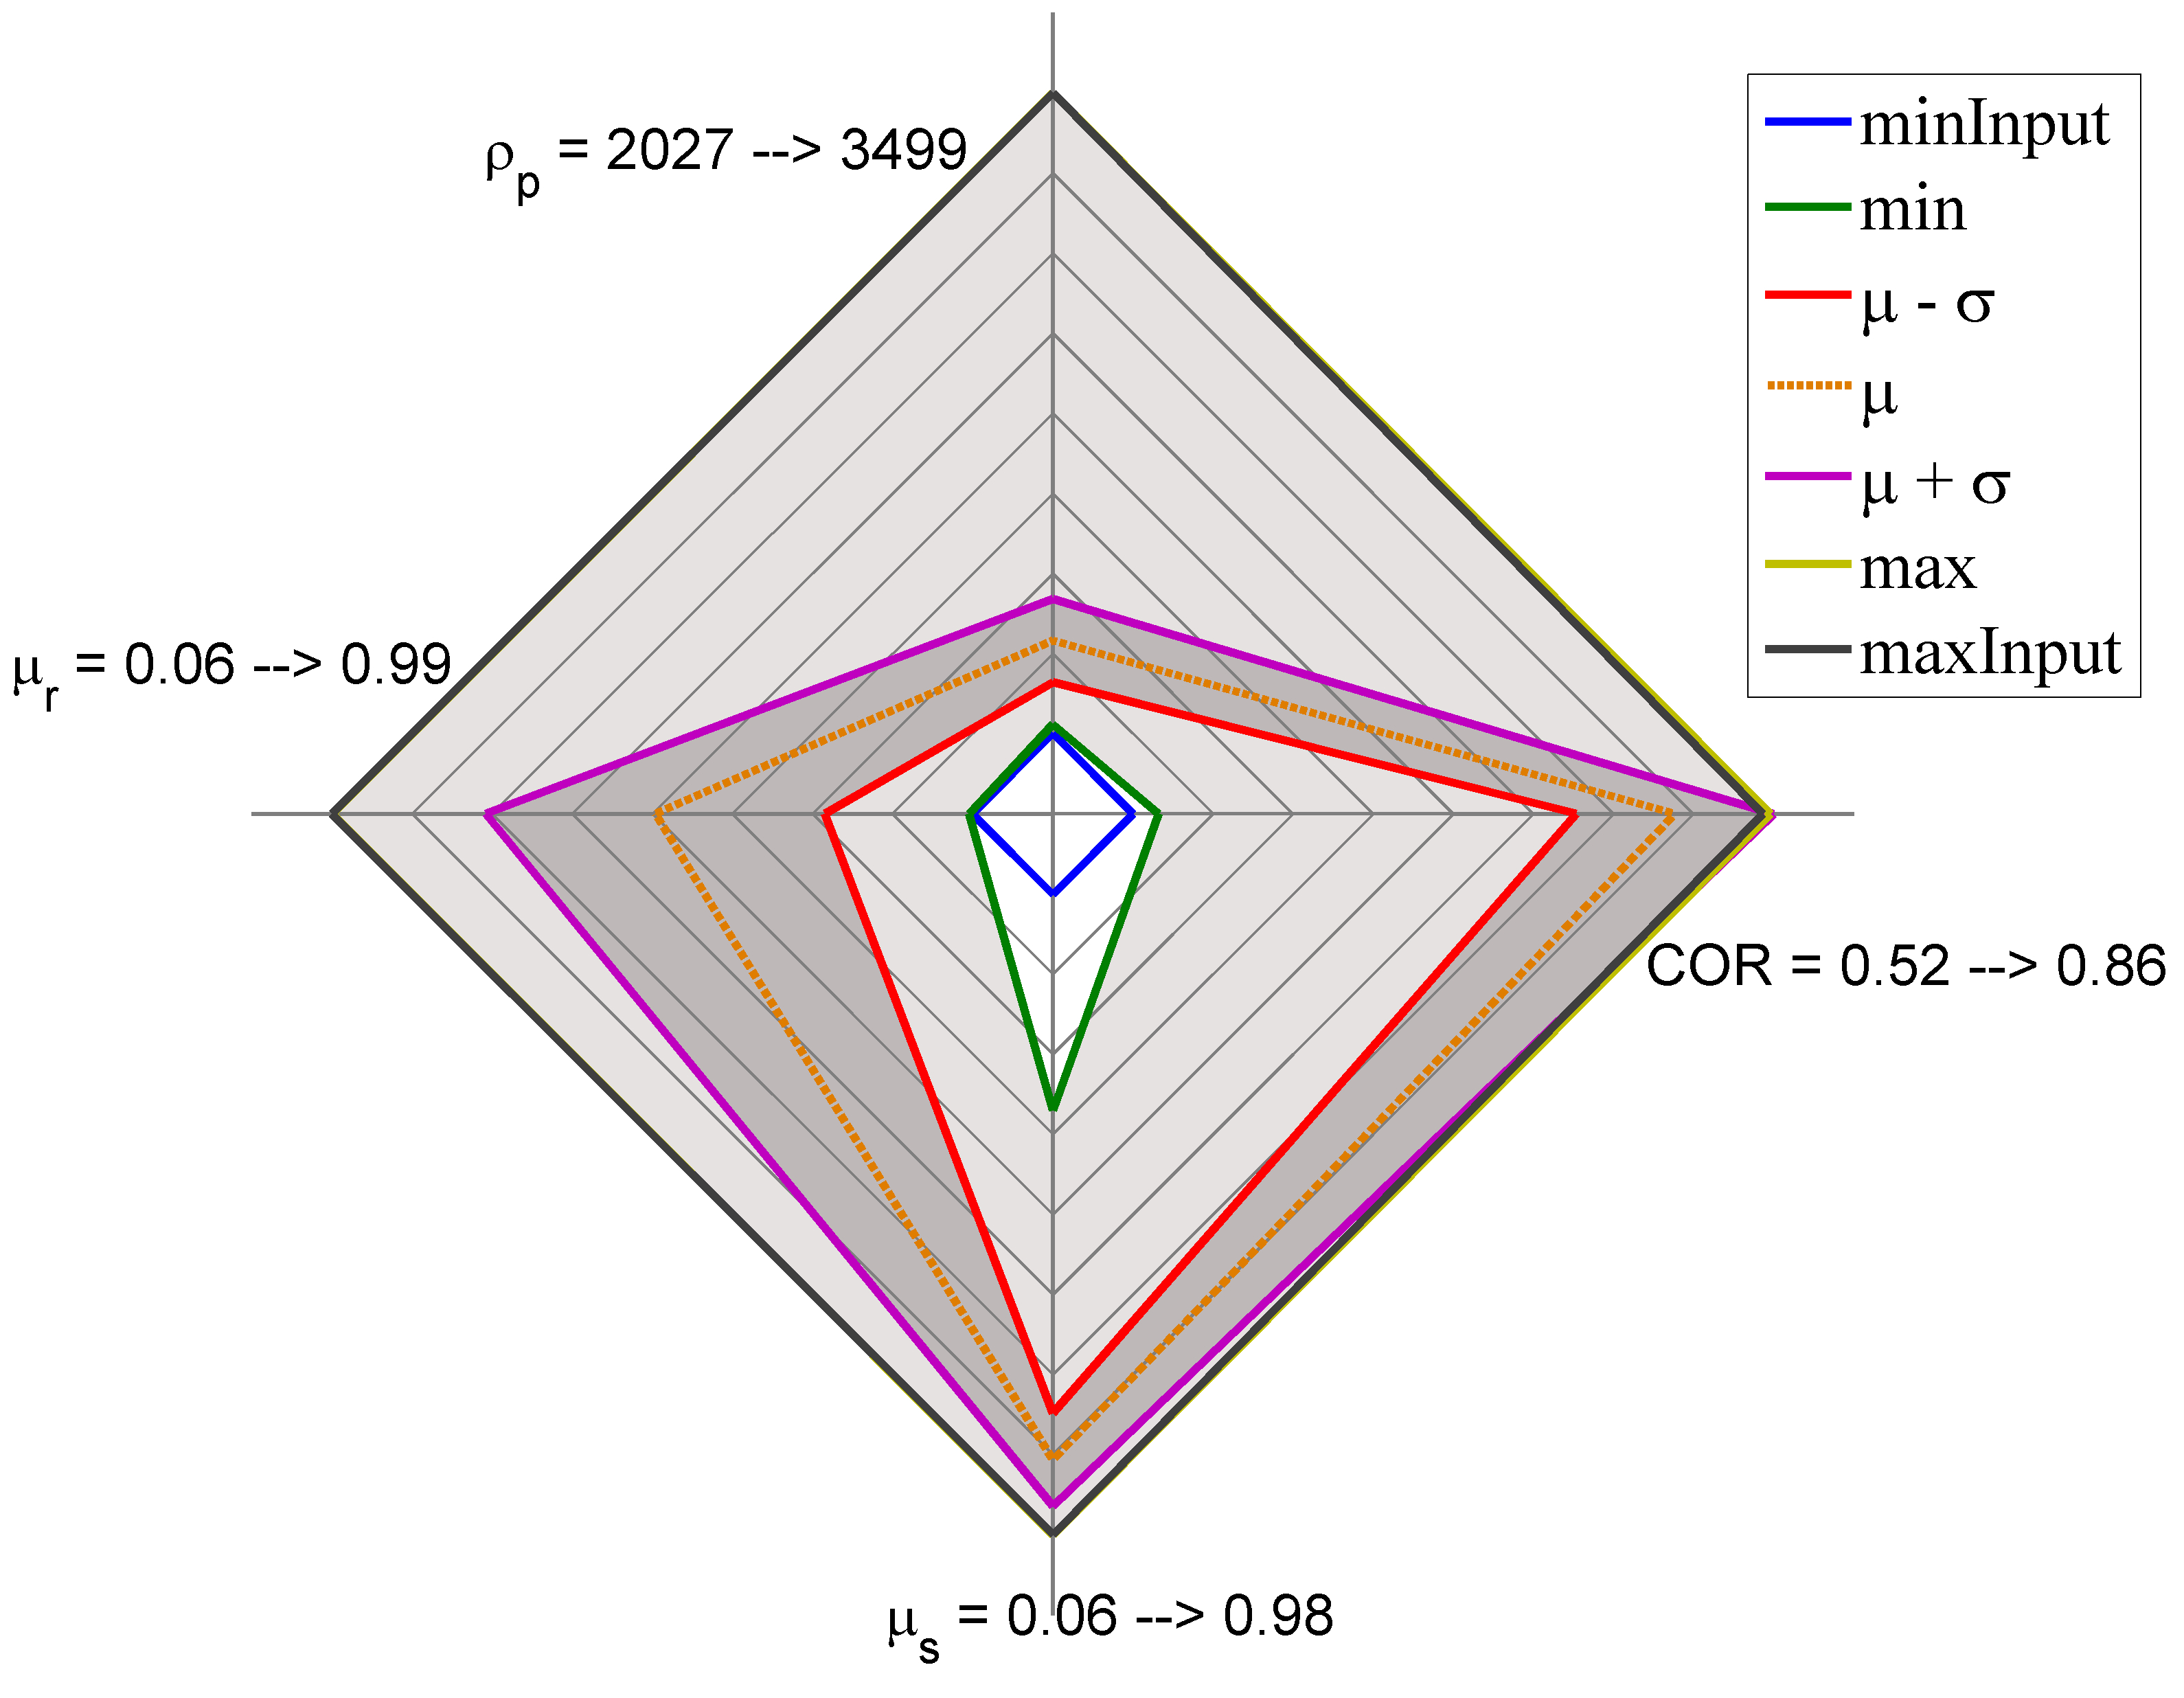
\includegraphics[width=\textwidth]{images/original/28radarpirker12schulze10070}
        \caption{Radar P12 Schulze10070}
        \label{fig:28radarpirker12schulze10070} 
    \end{subfigure}
    \begin{subfigure}[b]{0.48\columnwidth}
        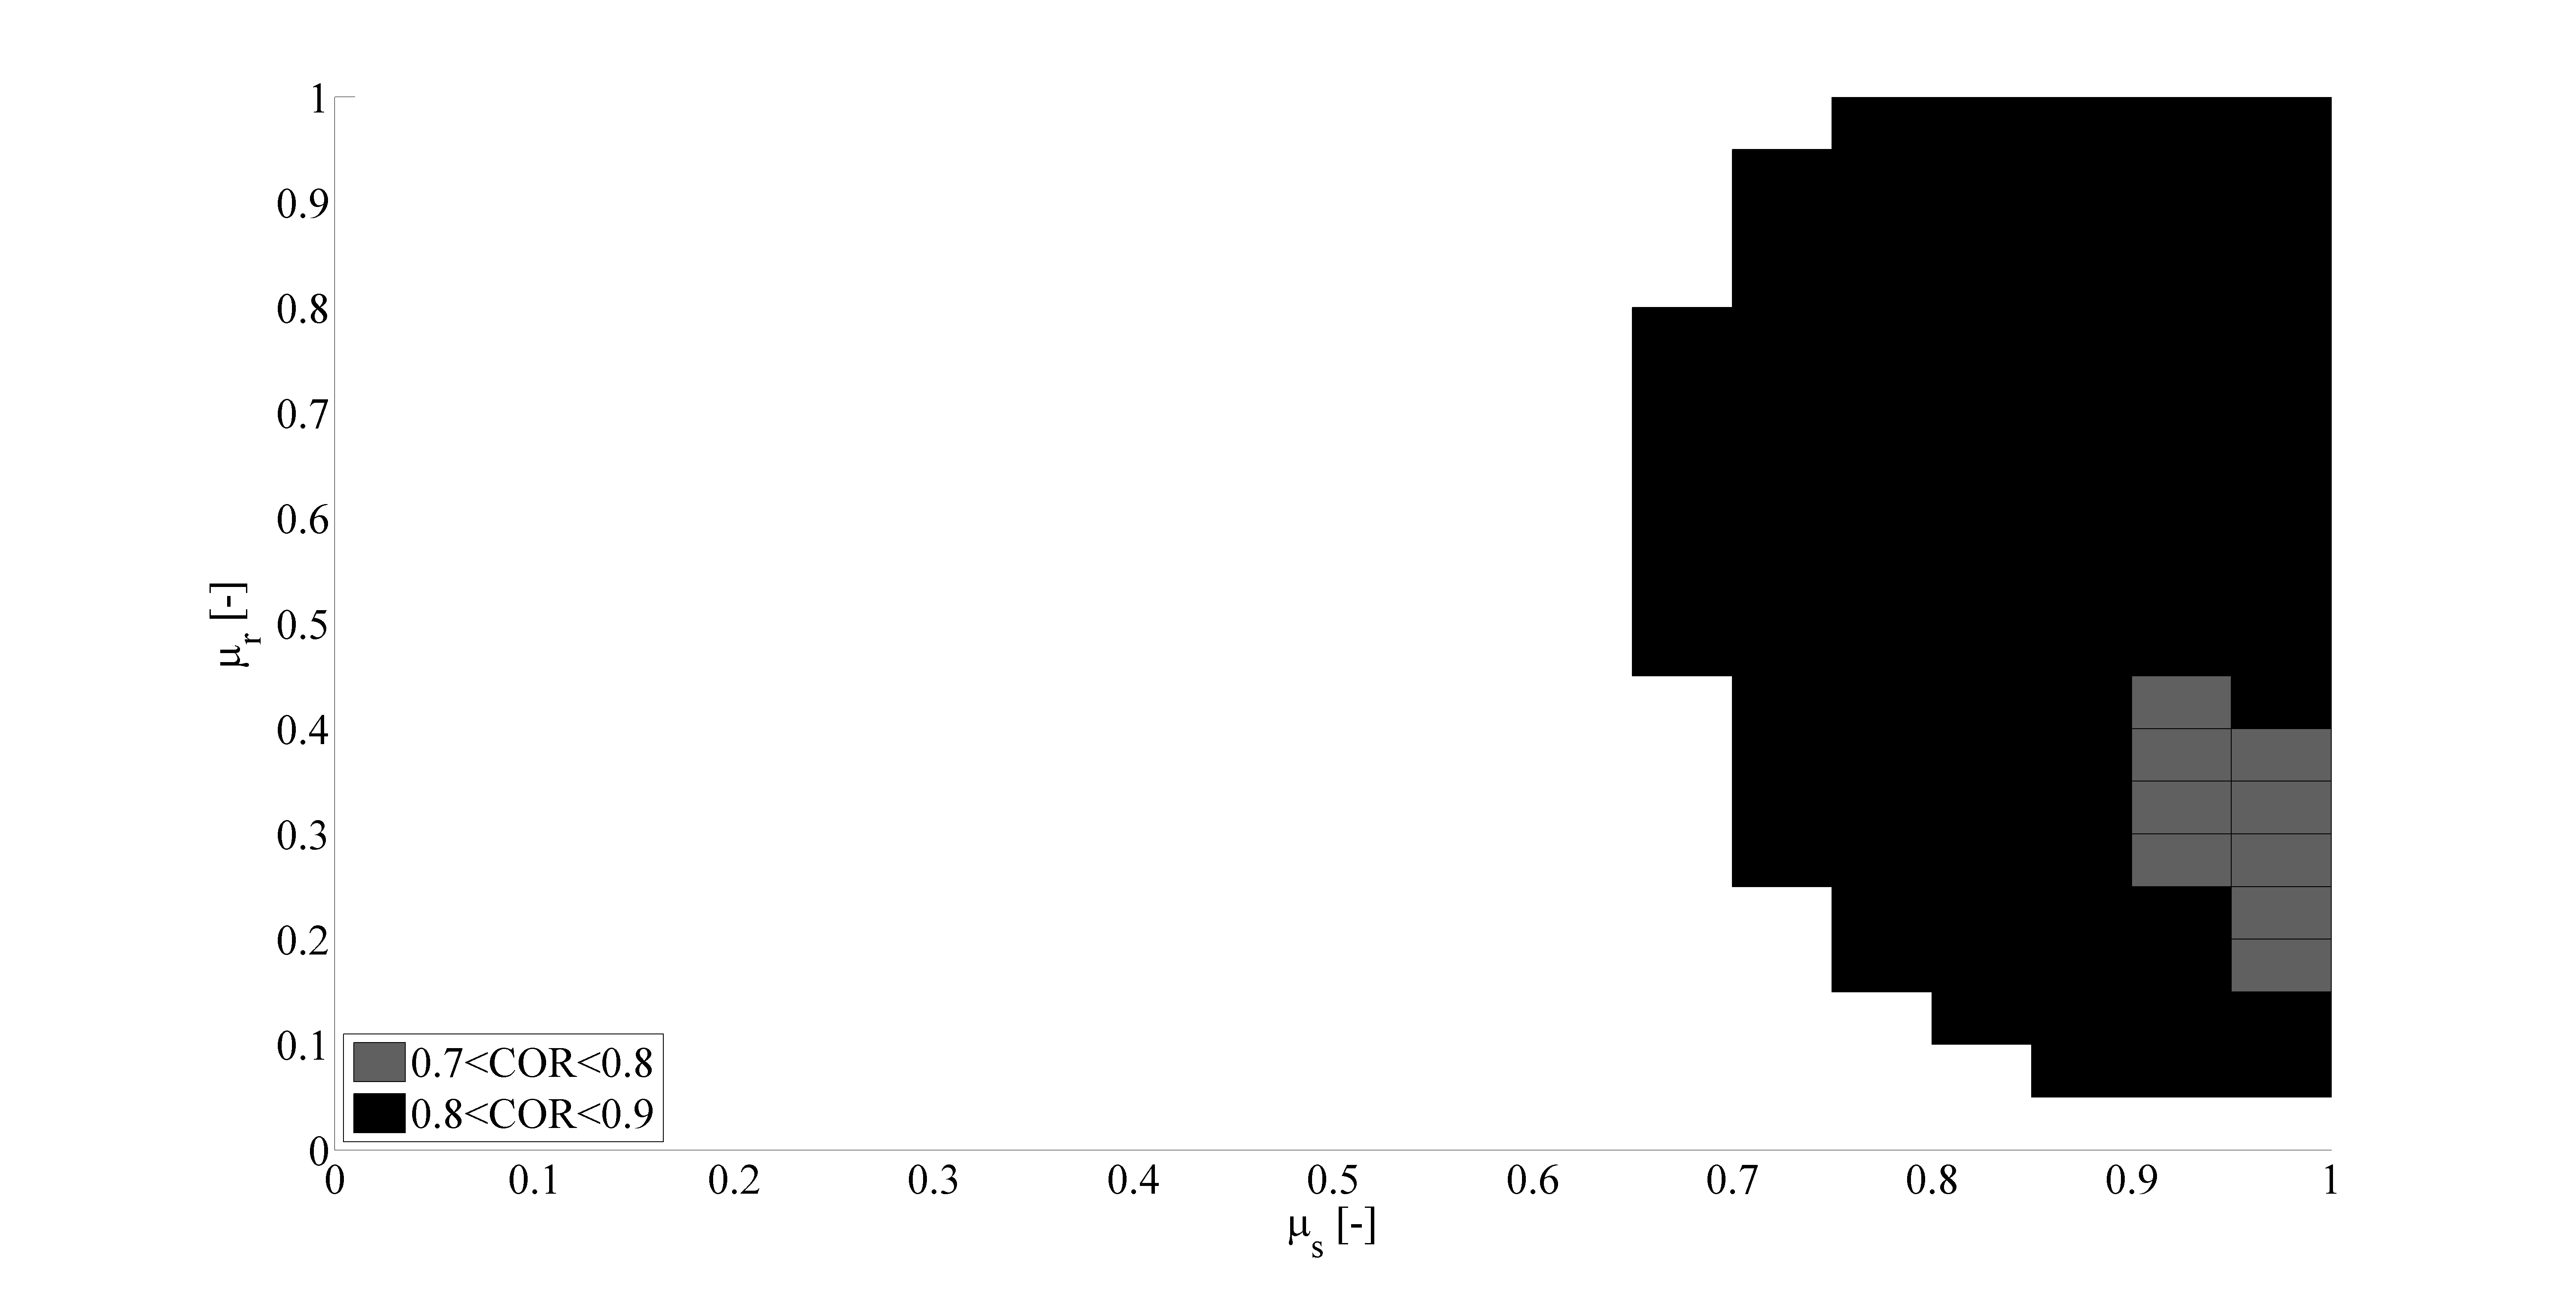
\includegraphics[width=\textwidth]{images/original/30cloudpirker12schulze10070}
        \caption{Cloud P12 Schulze10070}
        \label{fig:30cloudpirker12schulze10070} 
    \end{subfigure}
    \caption{Comparison between the original experimental selection P=1 and the
    increased and decreased results.}
    \label{fig:29schulzeradarandcloud}
\end{figure}
\begin{figure}[htp] \centering
    \begin{subfigure}[b]{0.48\columnwidth}
        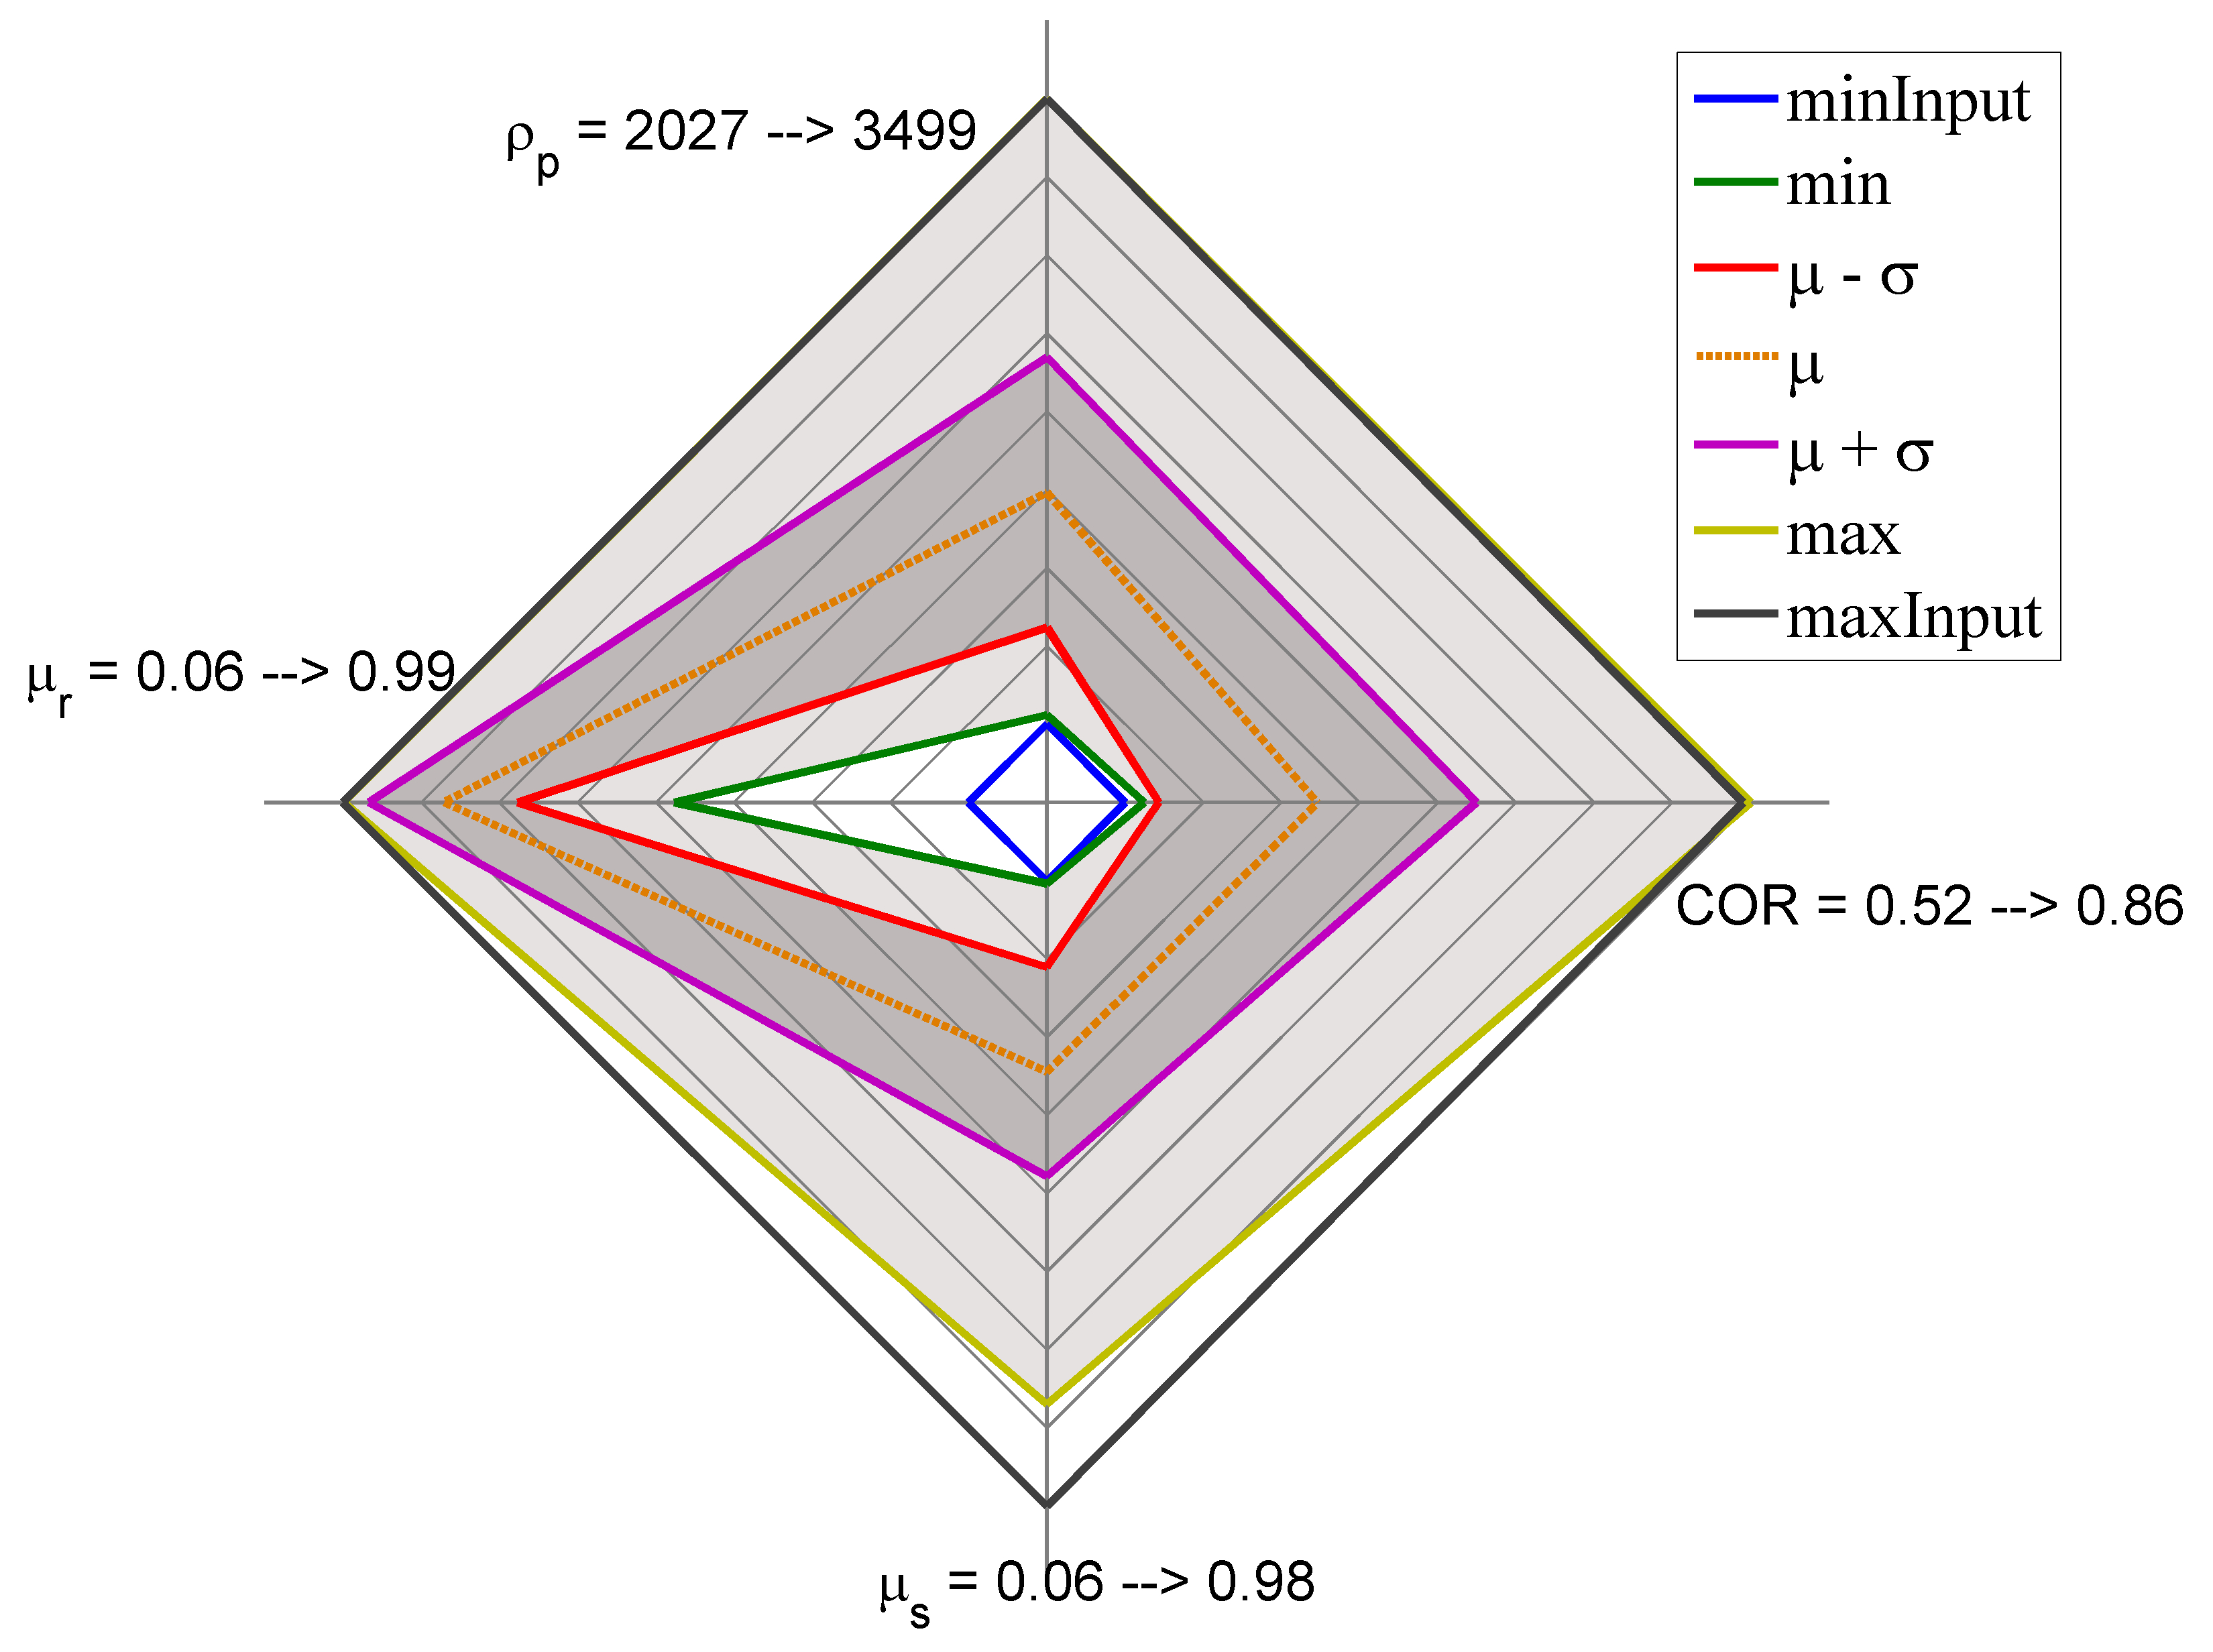
\includegraphics[width=\textwidth]{images/original/31radarpirker1aor}
        \caption{Radar P1 AOR}
        \label{fig:31radarpirker1aor} 
    \end{subfigure}
    \begin{subfigure}[b]{0.48\columnwidth}
        \includegraphics[width=\textwidth]{images/original/32cloudpirker1aor}
        \caption{Cloud P1 AOR}
        \label{fig:32cloudpirker1aor} 
    \end{subfigure}\\
        \begin{subfigure}[b]{0.48\columnwidth}
        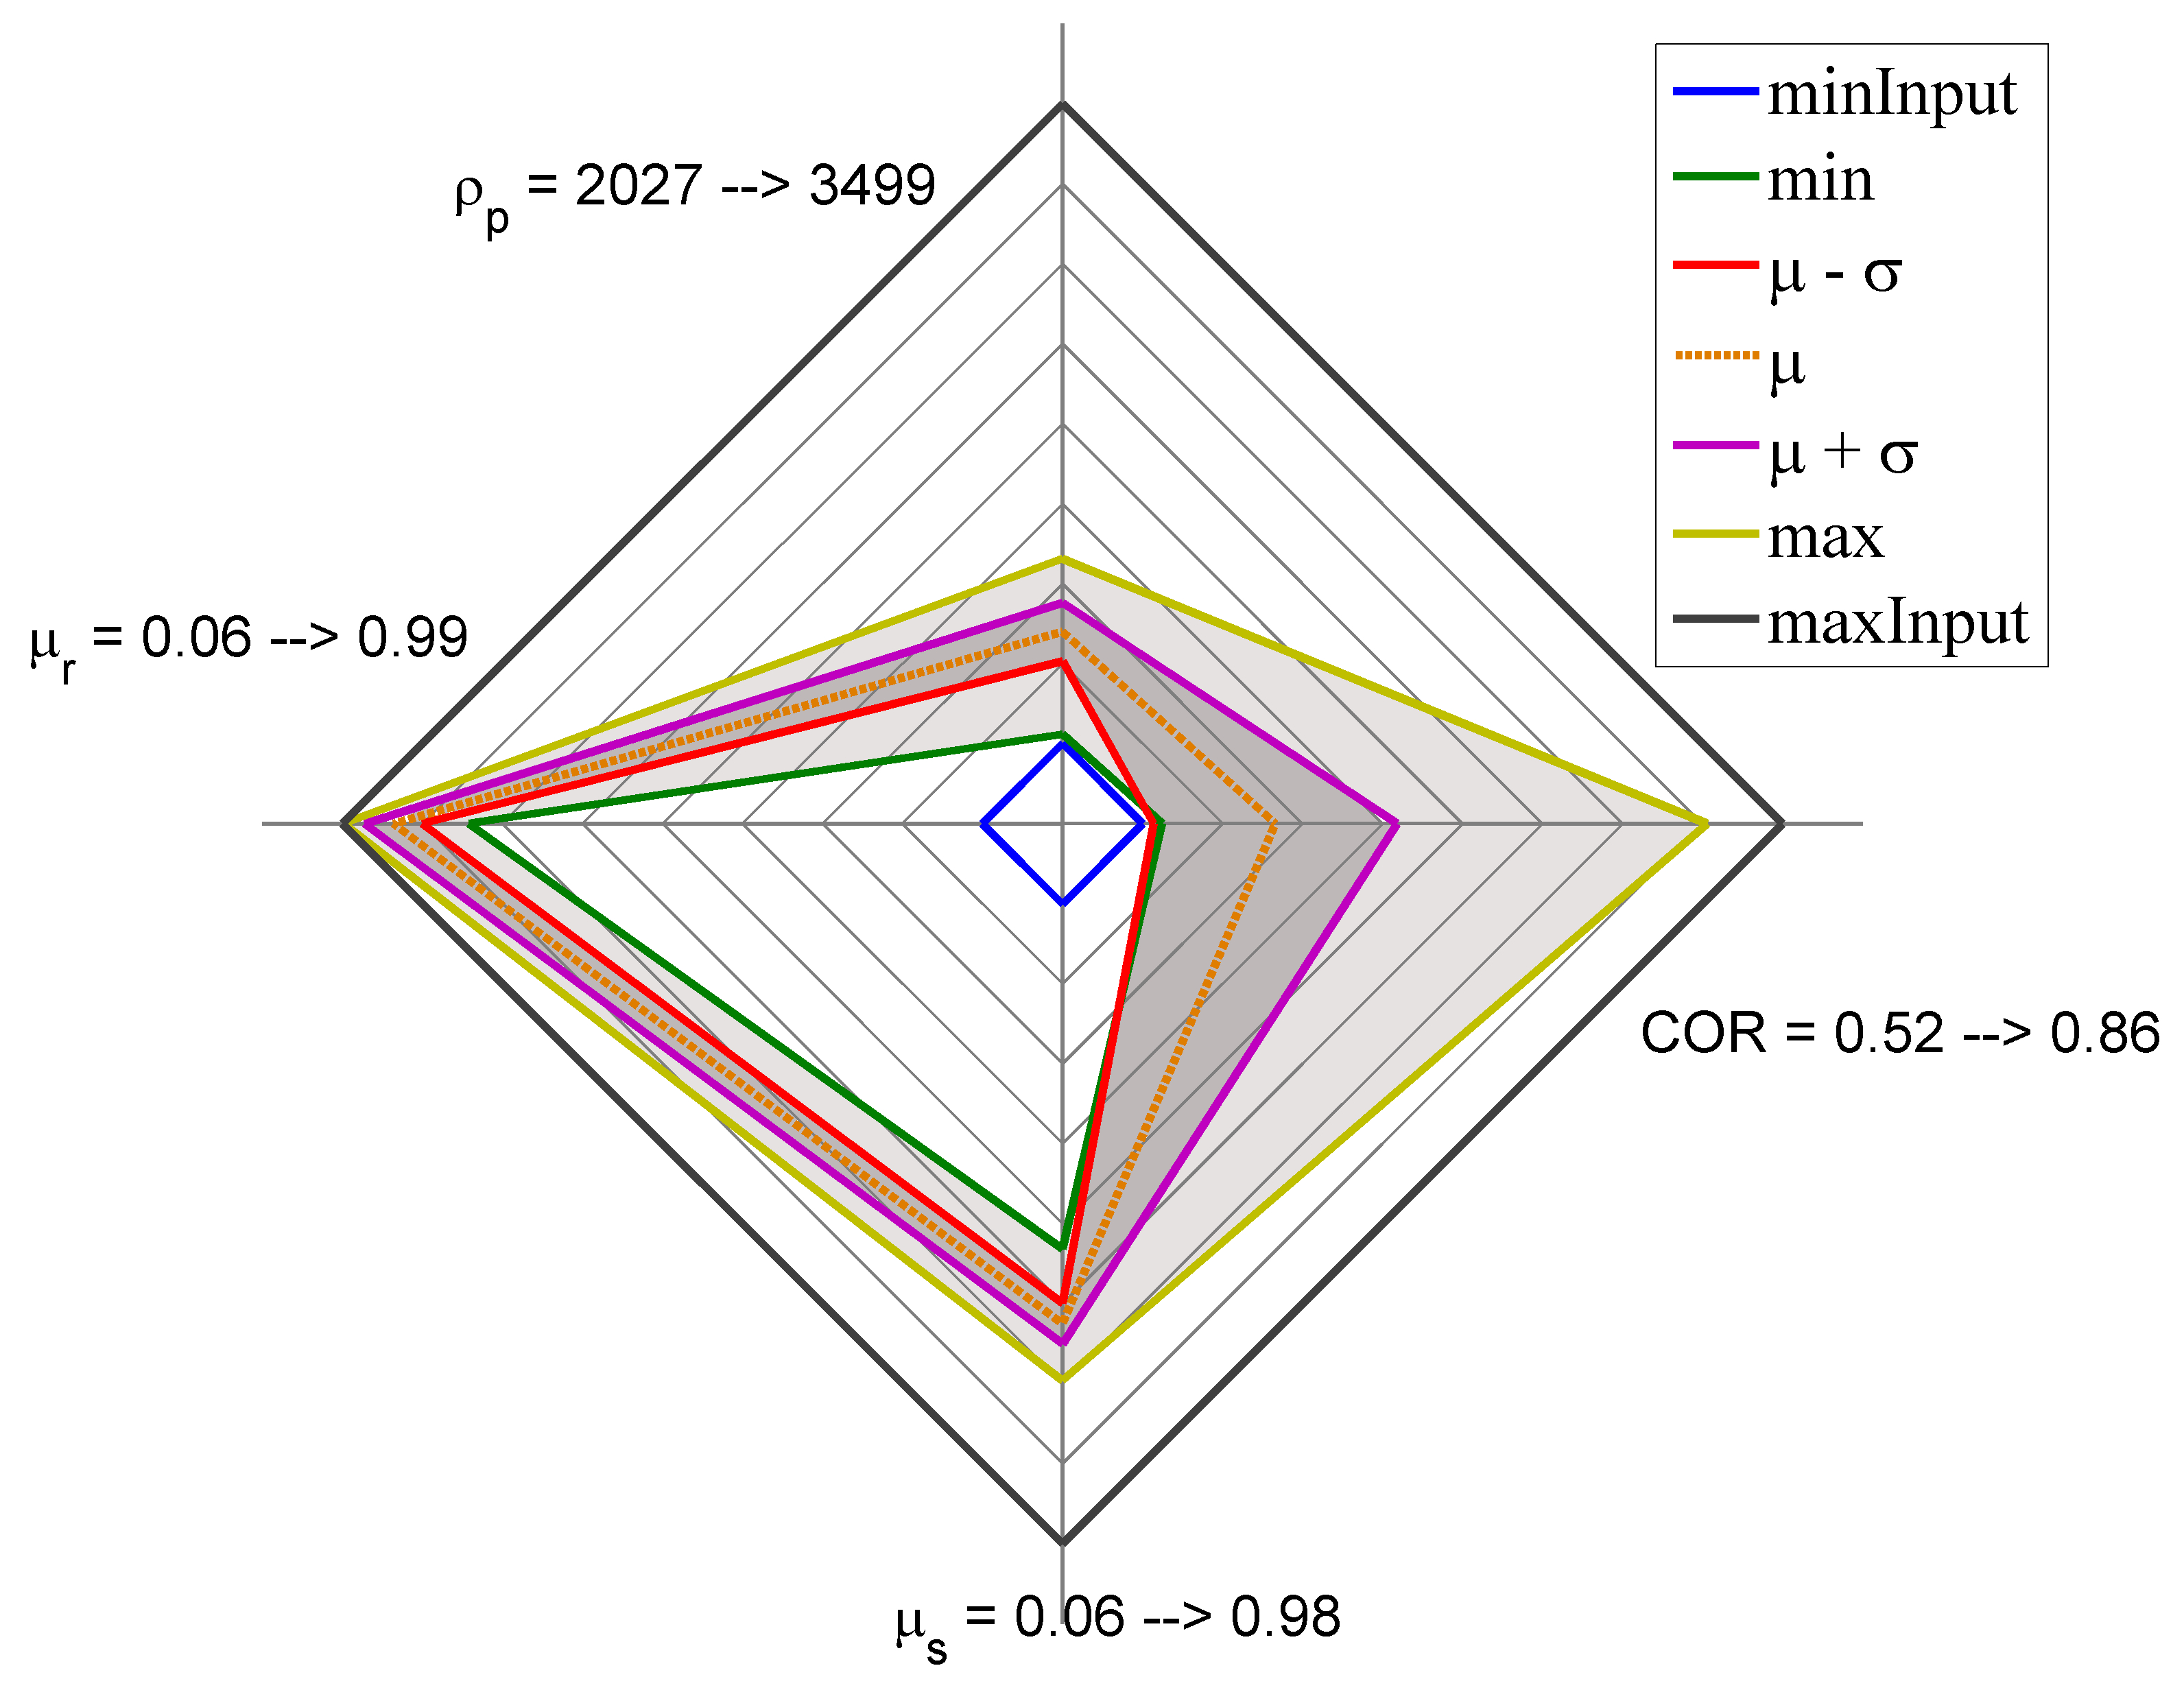
\includegraphics[width=\textwidth]{images/original/33radarpirker1schulze10070aor}
        \caption{Radar P1 Schulze 10070 & AOR}
        \label{fig:33radarpirker1schulze10070aor} 
    \end{subfigure}
    \begin{subfigure}[b]{0.48\columnwidth}
        \includegraphics[width=\textwidth]{images/original/34cloudpirker1schulze10070aor}
        \caption{Cloud P1 Schulze 10070 & AOR}
        \label{fig:34cloudpirker1schulze10070aor} 
    \end{subfigure}
    \caption{AOR and merge results.}
    \label{fig:35schulze10070aorradarandcloud}
\end{figure}


%\begin{figure}[!h] 
\centering 
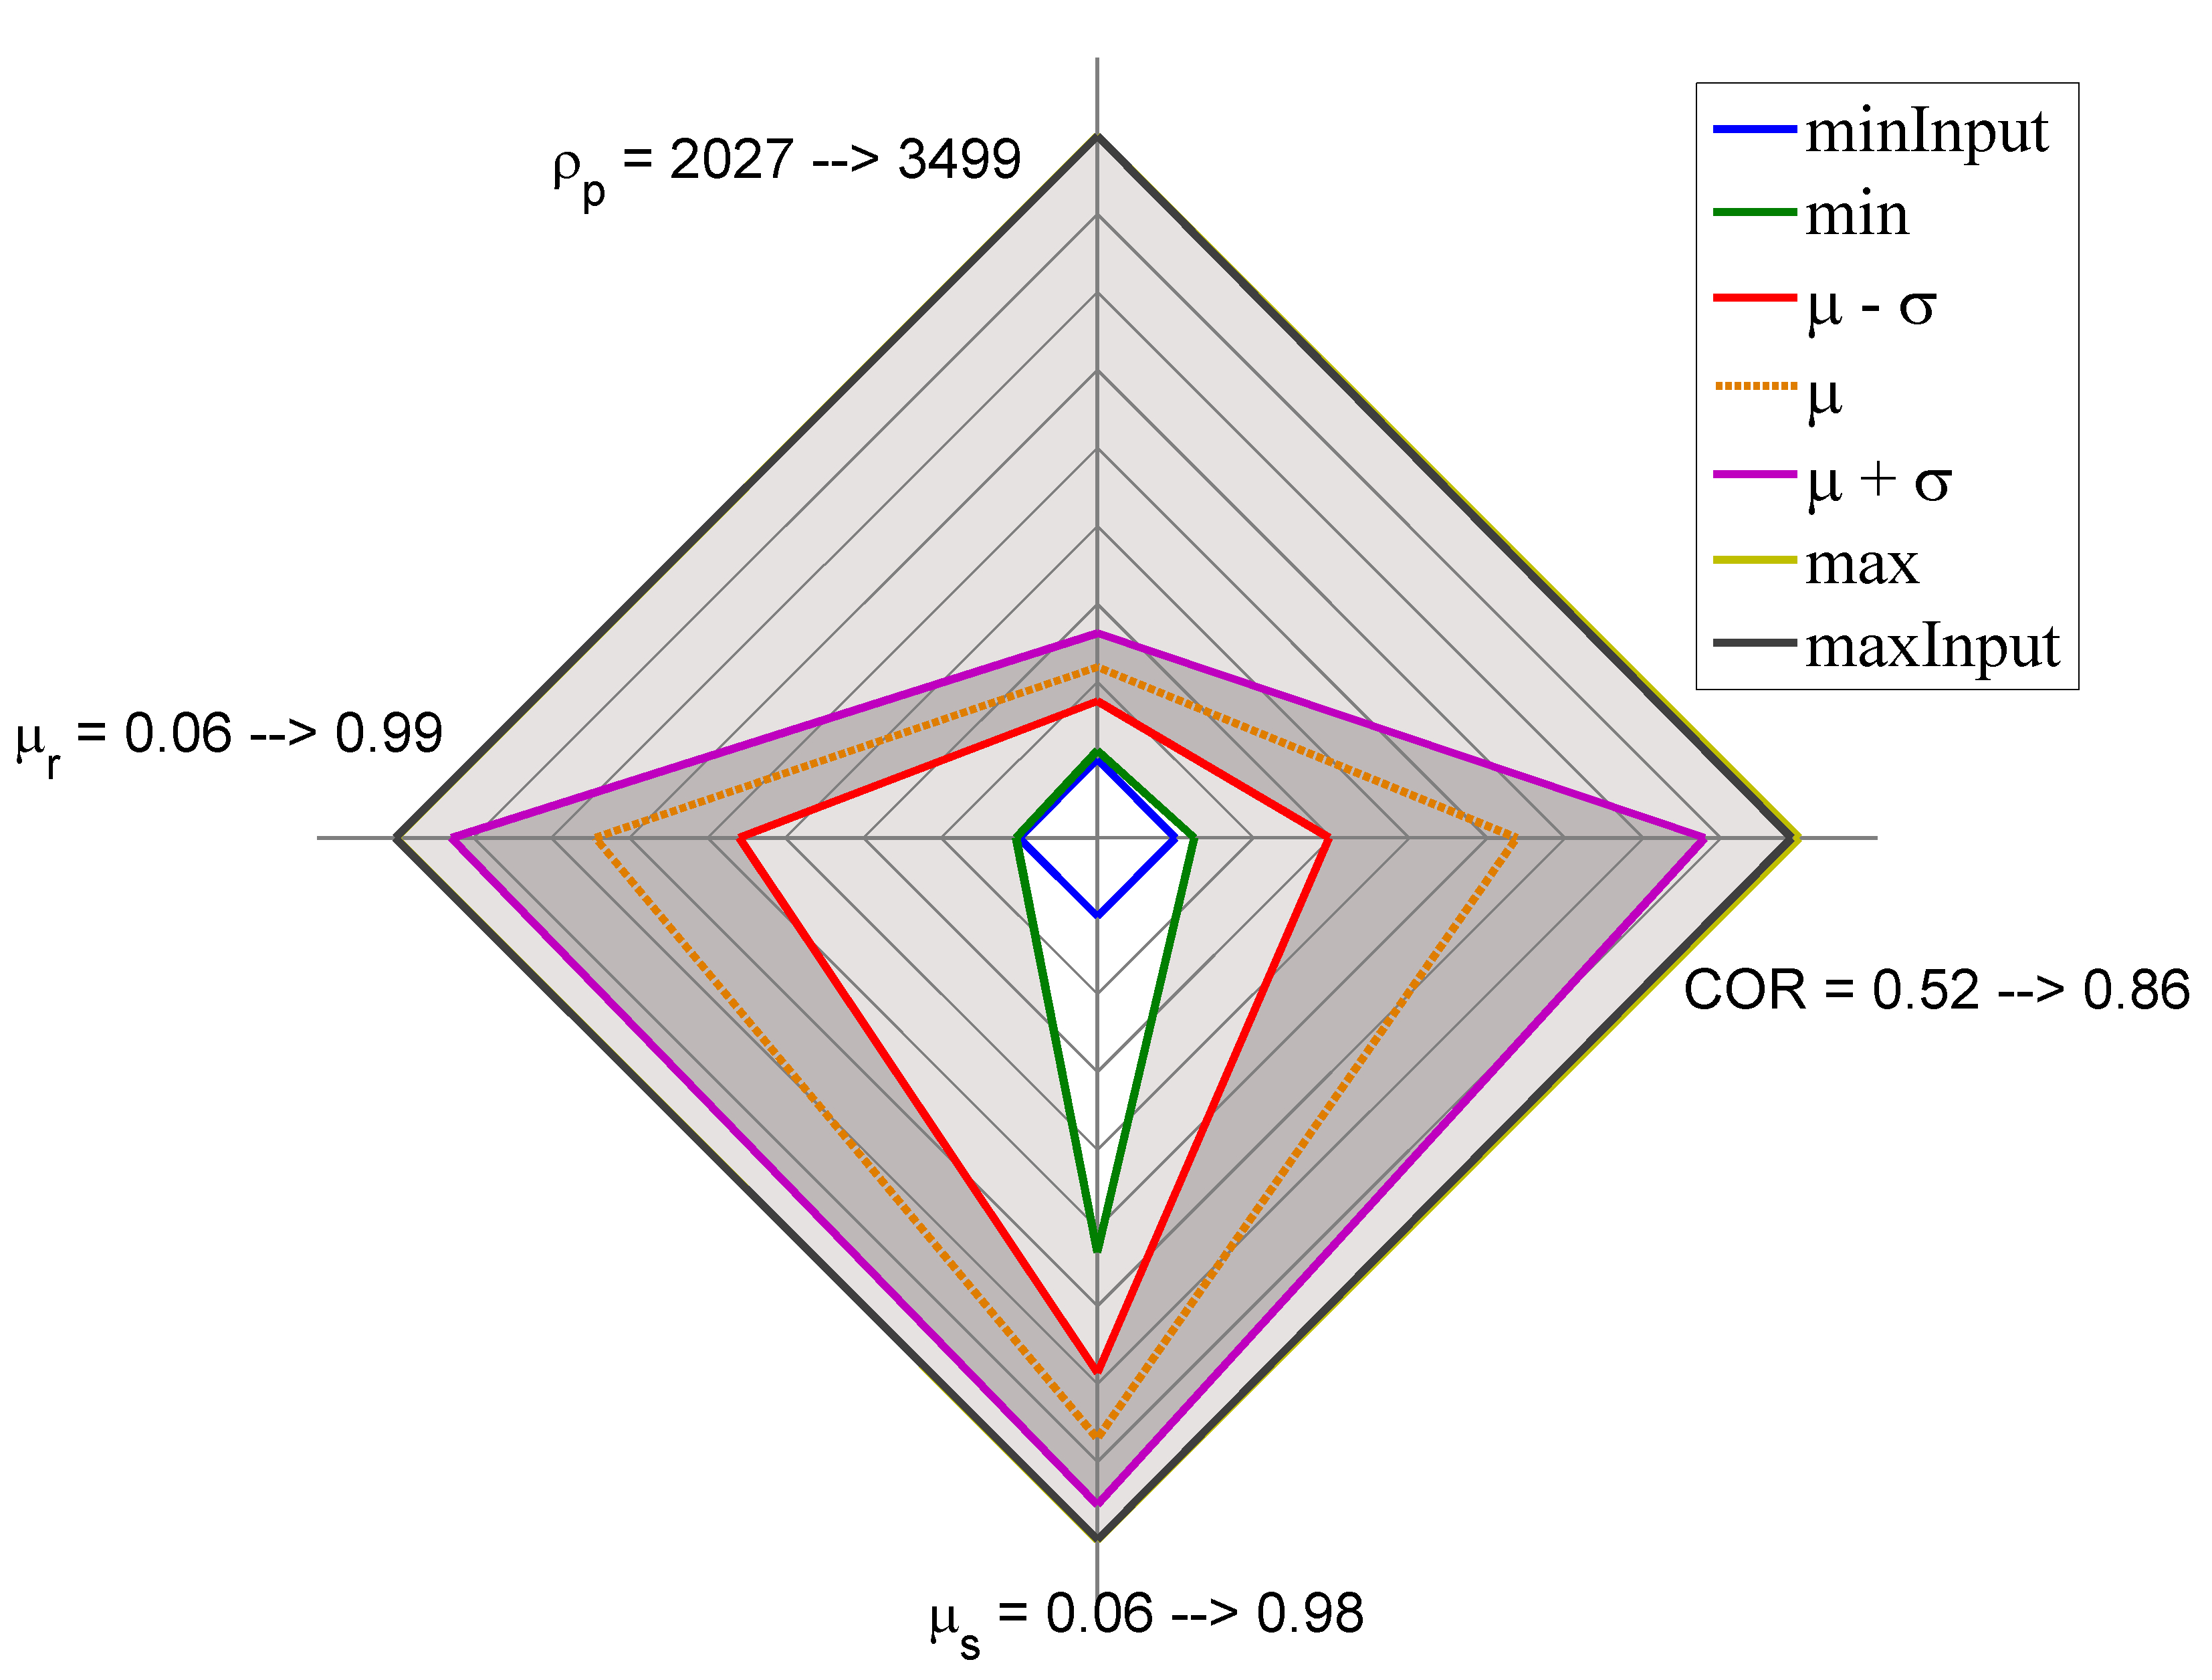
\includegraphics[height=0.40\columnwidth]{images/original/24radarpirker1schulze10070}
%[width=.96\textwidth]
\caption{Radar P1 Schulze10070}
\label{fig:24radarpirker1schulze10070} 
\end{figure}

%SCT: sn = 10070 [Pa], coeff. P. = 1
% \begin{figure}[htp]
%     \centering
%     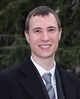
\includegraphics[width=.2\textwidth]{images/vitae/lbenvenuti}
%     \caption{OpenMP, MPI, MPI/OpenMP Hybrid runs of Box in a box testcase on 32
%     cores. The OpenMP-only run suffers from limited memory bandwidth in
%     memory-bound algorithms inside of the Modify section of the code. MPI-only has
%     low averaged runtimes for each section, but a very large Other timing, which
%     hints for a large amount of load-imbalance. Hybrid timings are a bit worse
%     on average, but because of better balancing, processes have lower wait times
%     inside of Other timing.}
% 	\label{fig:boxInBoxComparison}

%\begin{figure}[!h] 
\centering 
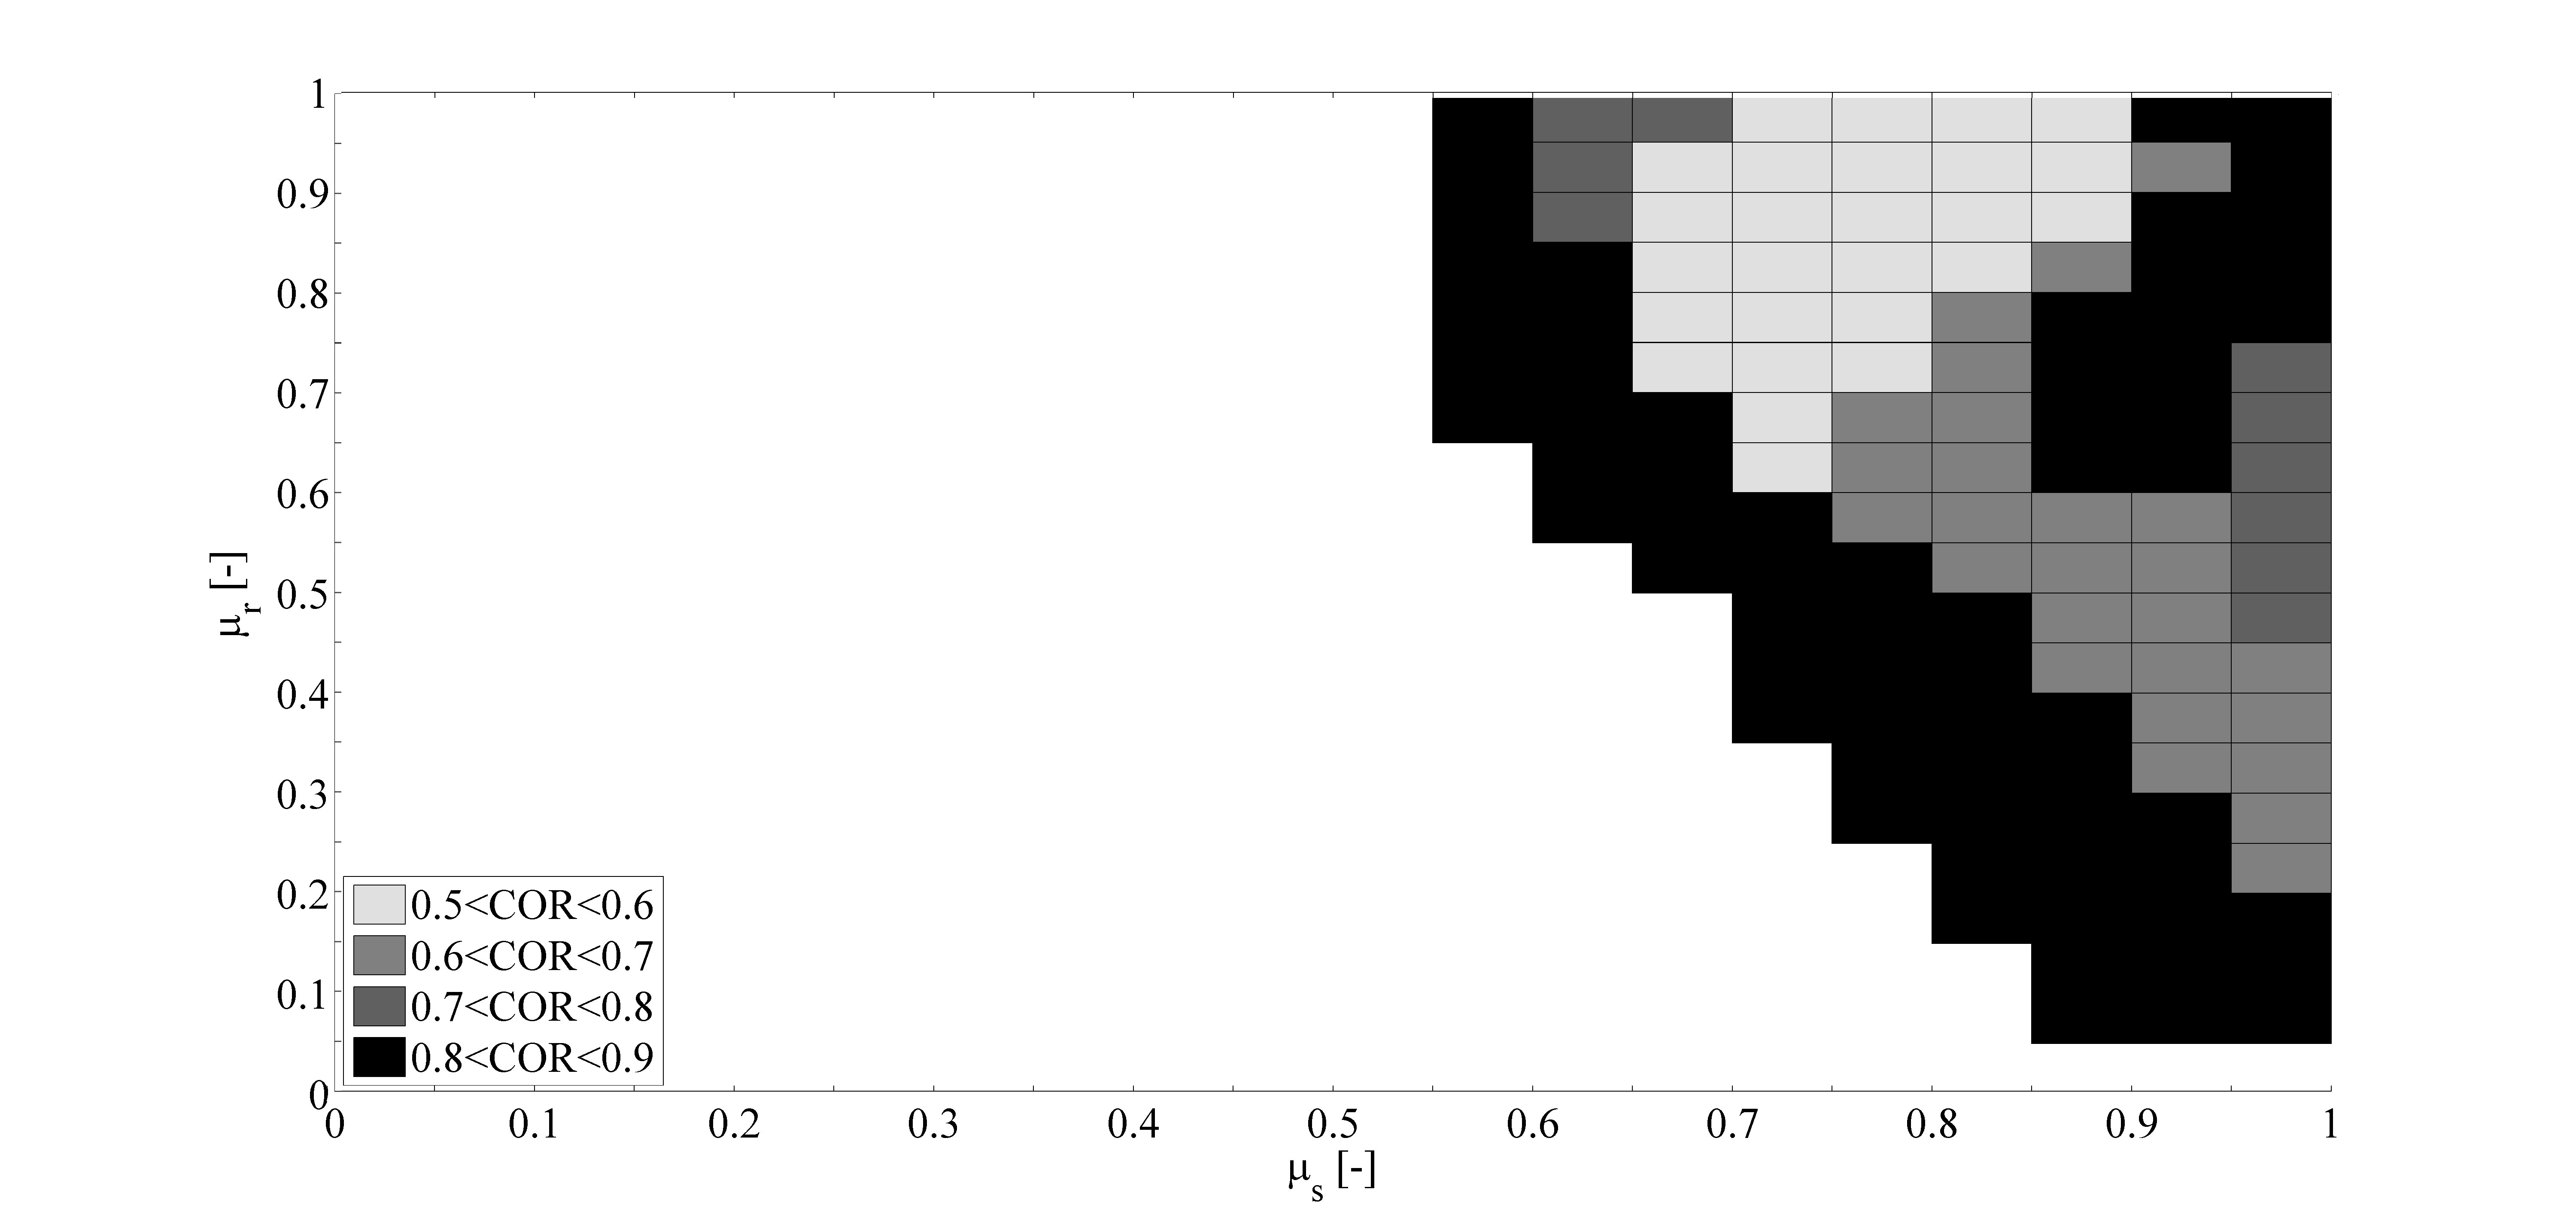
\includegraphics[height=0.33\columnwidth]{images/original/25cloudpirker1schulze10070}
%[width=.96\textwidth]
\caption{Cloud P1 Schulze10070}
\label{fig:25cloudpirker1schulze10070} 
\end{figure}

%SCT: sn = 10070 [Pa], coeff. P. = 1
% \begin{figure}[htp]
%     \centering
%     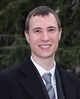
\includegraphics[width=.2\textwidth]{images/vitae/lbenvenuti}
%     \caption{OpenMP, MPI, MPI/OpenMP Hybrid runs of Box in a box testcase on 32
%     cores. The OpenMP-only run suffers from limited memory bandwidth in
%     memory-bound algorithms inside of the Modify section of the code. MPI-only has
%     low averaged runtimes for each section, but a very large Other timing, which
%     hints for a large amount of load-imbalance. Hybrid timings are a bit worse
%     on average, but because of better balancing, processes have lower wait times
%     inside of Other timing.}
% 	\label{fig:boxInBoxComparison}

%\begin{figure}[!h] 
\centering 
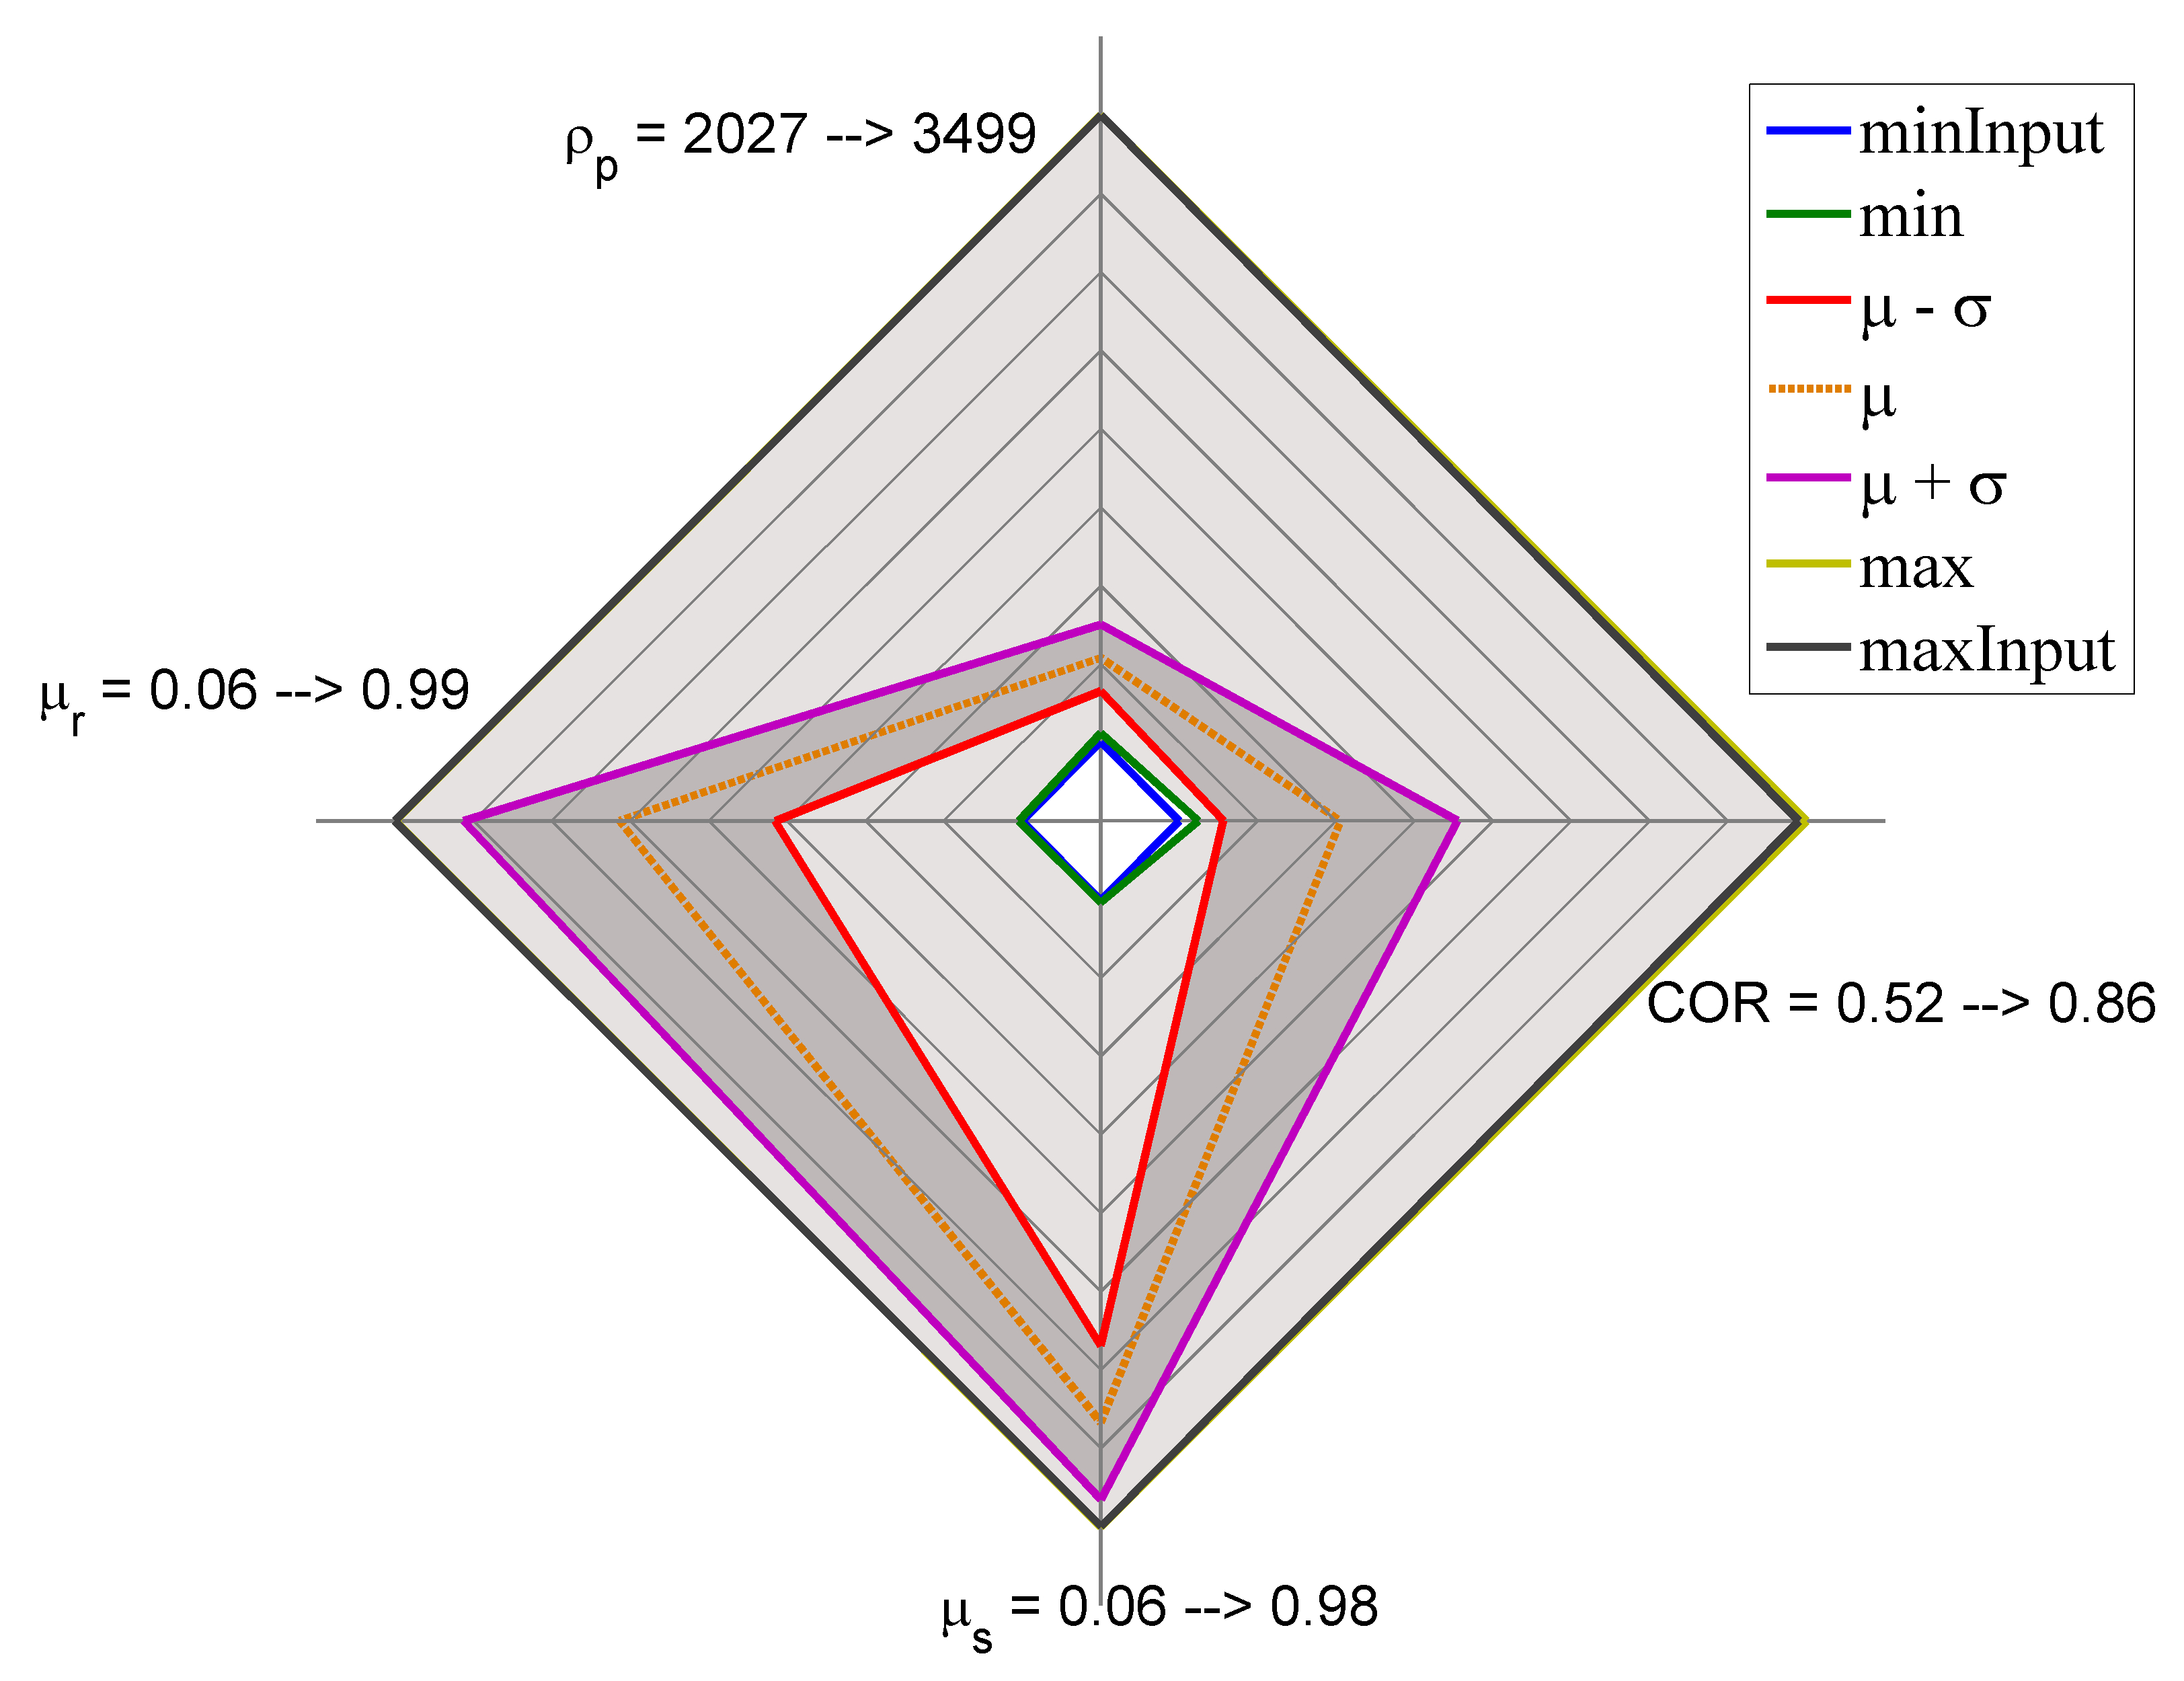
\includegraphics[height=3in]{images/original/26radarpirker08schulze10070}
%[width=.96\textwidth]
\caption{Radar P08 Schulze10070}
\label{fig:26radarpirker08schulze10070} 
\end{figure}

%SCT: sn = 10070 [Pa], coeff. P. = 0.8
% \begin{figure}[htp]
%     \centering
%     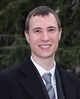
\includegraphics[width=.2\textwidth]{images/vitae/lbenvenuti}
%     \caption{OpenMP, MPI, MPI/OpenMP Hybrid runs of Box in a box testcase on 32
%     cores. The OpenMP-only run suffers from limited memory bandwidth in
%     memory-bound algorithms inside of the Modify section of the code. MPI-only has
%     low averaged runtimes for each section, but a very large Other timing, which
%     hints for a large amount of load-imbalance. Hybrid timings are a bit worse
%     on average, but because of better balancing, processes have lower wait times
%     inside of Other timing.}
% 	\label{fig:boxInBoxComparison}

%\begin{figure}[!h] 
\centering 
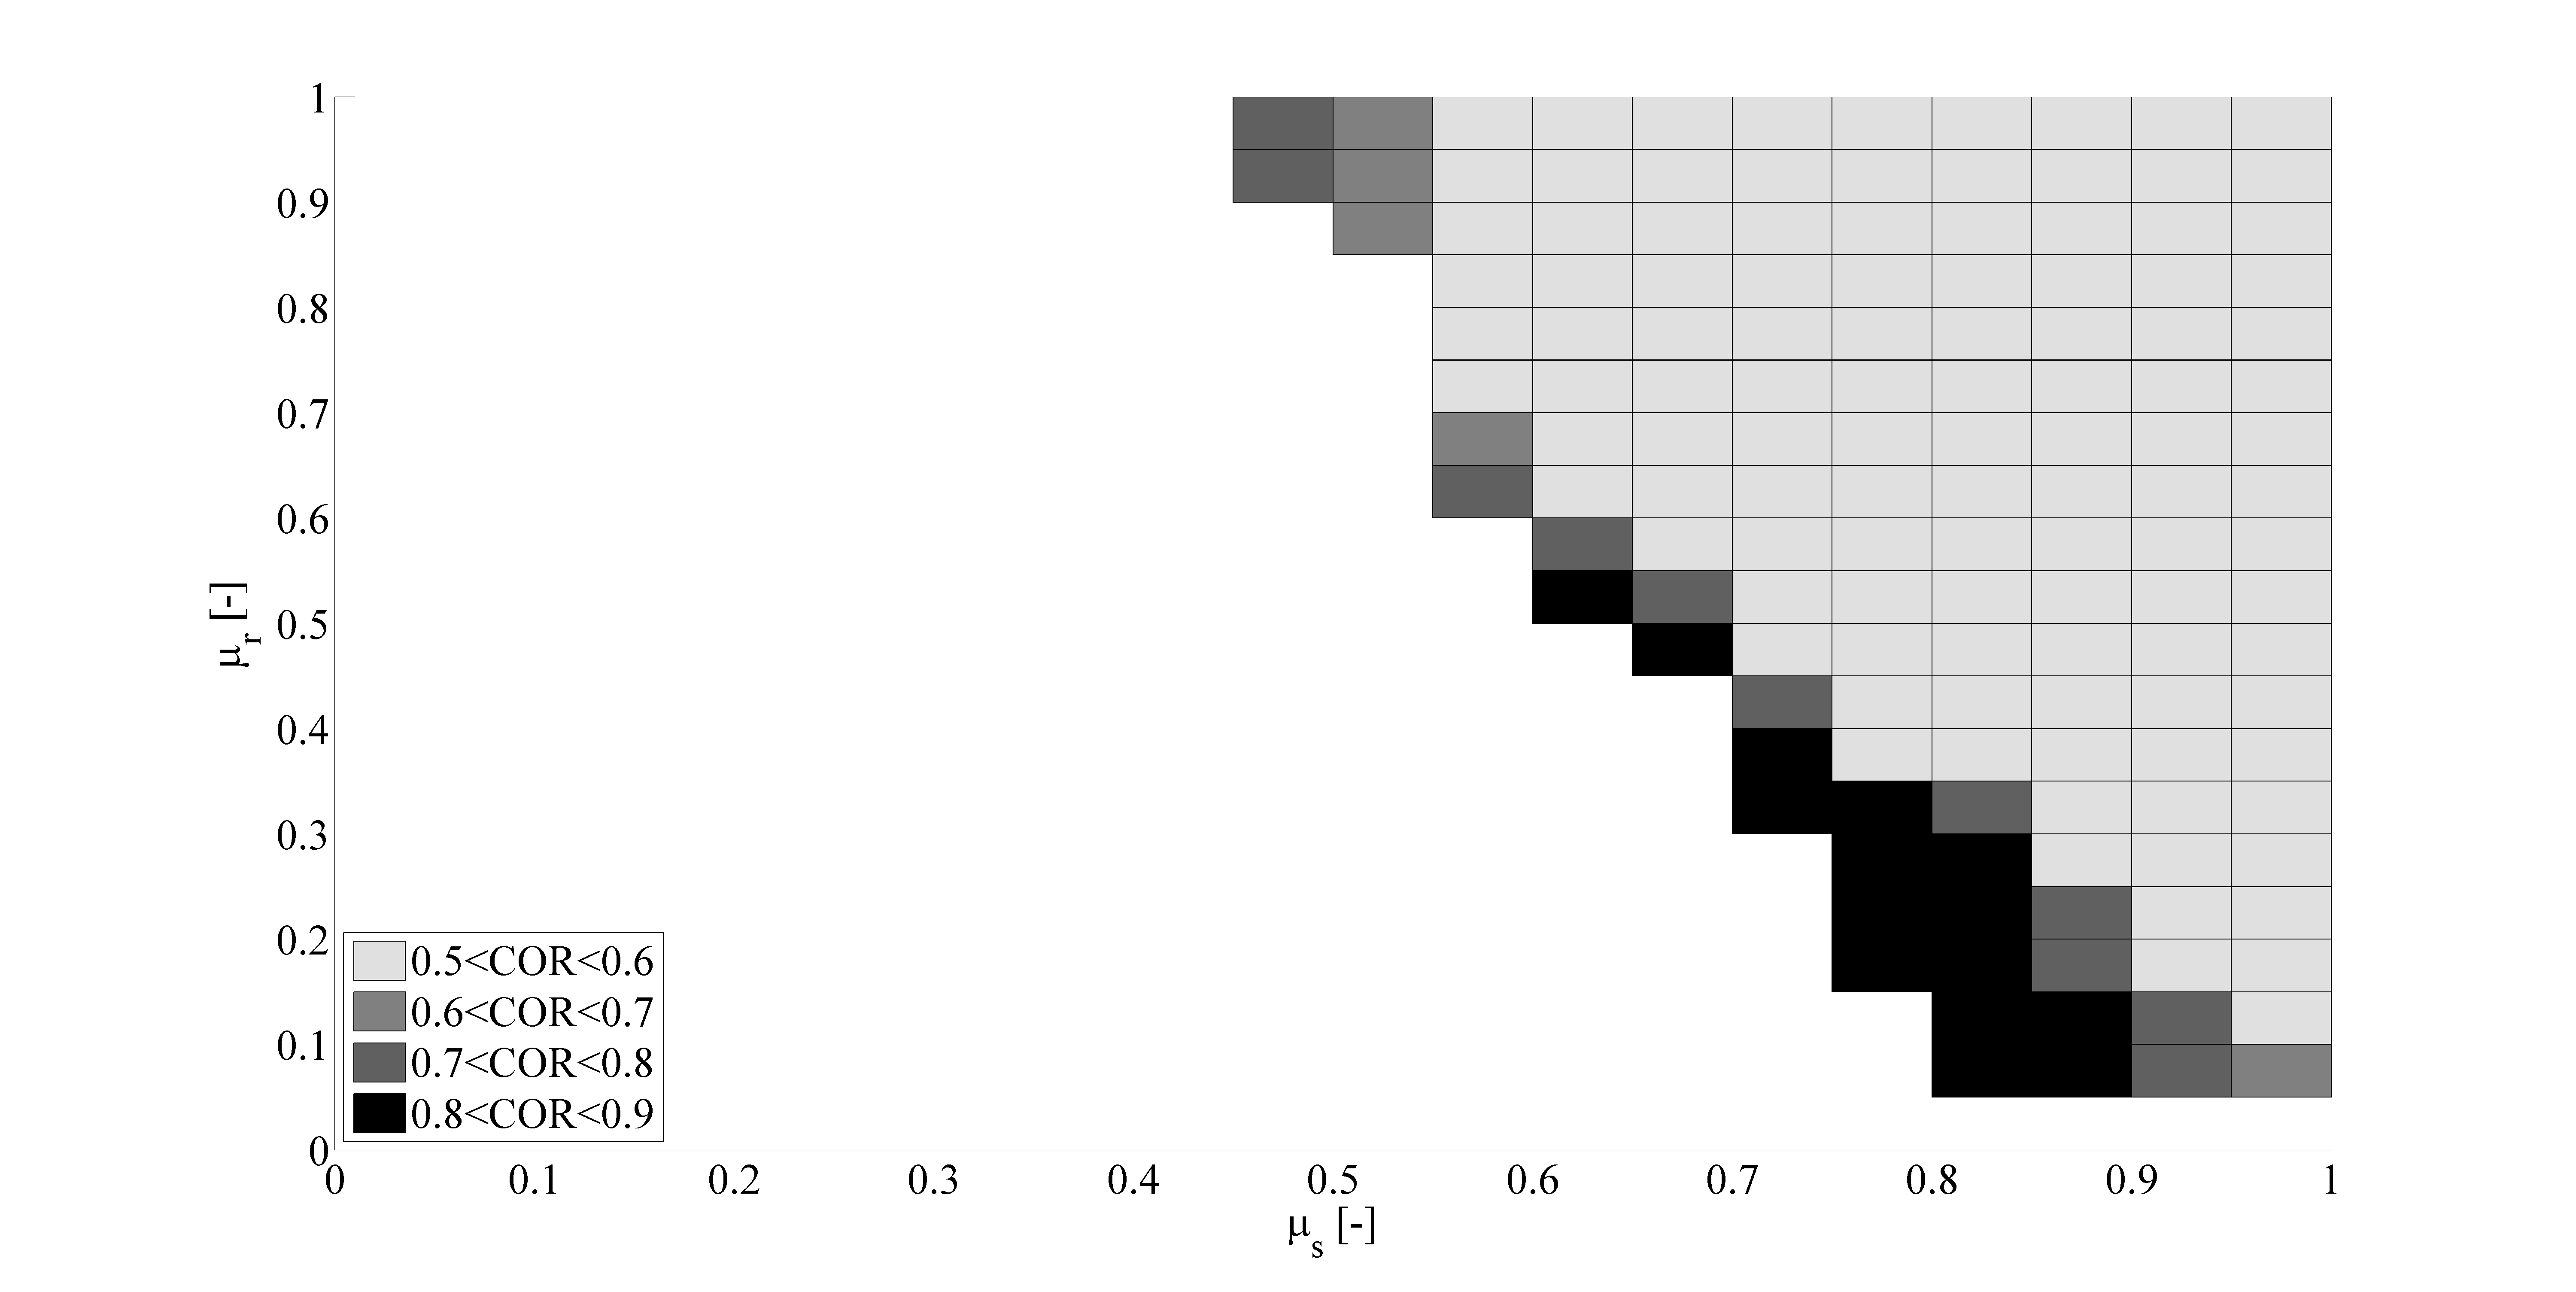
\includegraphics[height=3in]{images/original/27cloudpirker08schulze10070}
%[width=.96\textwidth]
\caption{Cloud P08 Schulze10070}
\label{fig:27cloudpirker08schulze10070} 
\end{figure}

%SCT: sn = 10070 [Pa], coeff. P. = 0.8
% \begin{figure}[htp]
%     \centering
%     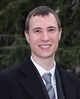
\includegraphics[width=.2\textwidth]{images/vitae/lbenvenuti}
%     \caption{OpenMP, MPI, MPI/OpenMP Hybrid runs of Box in a box testcase on 32
%     cores. The OpenMP-only run suffers from limited memory bandwidth in
%     memory-bound algorithms inside of the Modify section of the code. MPI-only has
%     low averaged runtimes for each section, but a very large Other timing, which
%     hints for a large amount of load-imbalance. Hybrid timings are a bit worse
%     on average, but because of better balancing, processes have lower wait times
%     inside of Other timing.}
% 	\label{fig:boxInBoxComparison}

%\begin{figure}[!h] 
\centering 
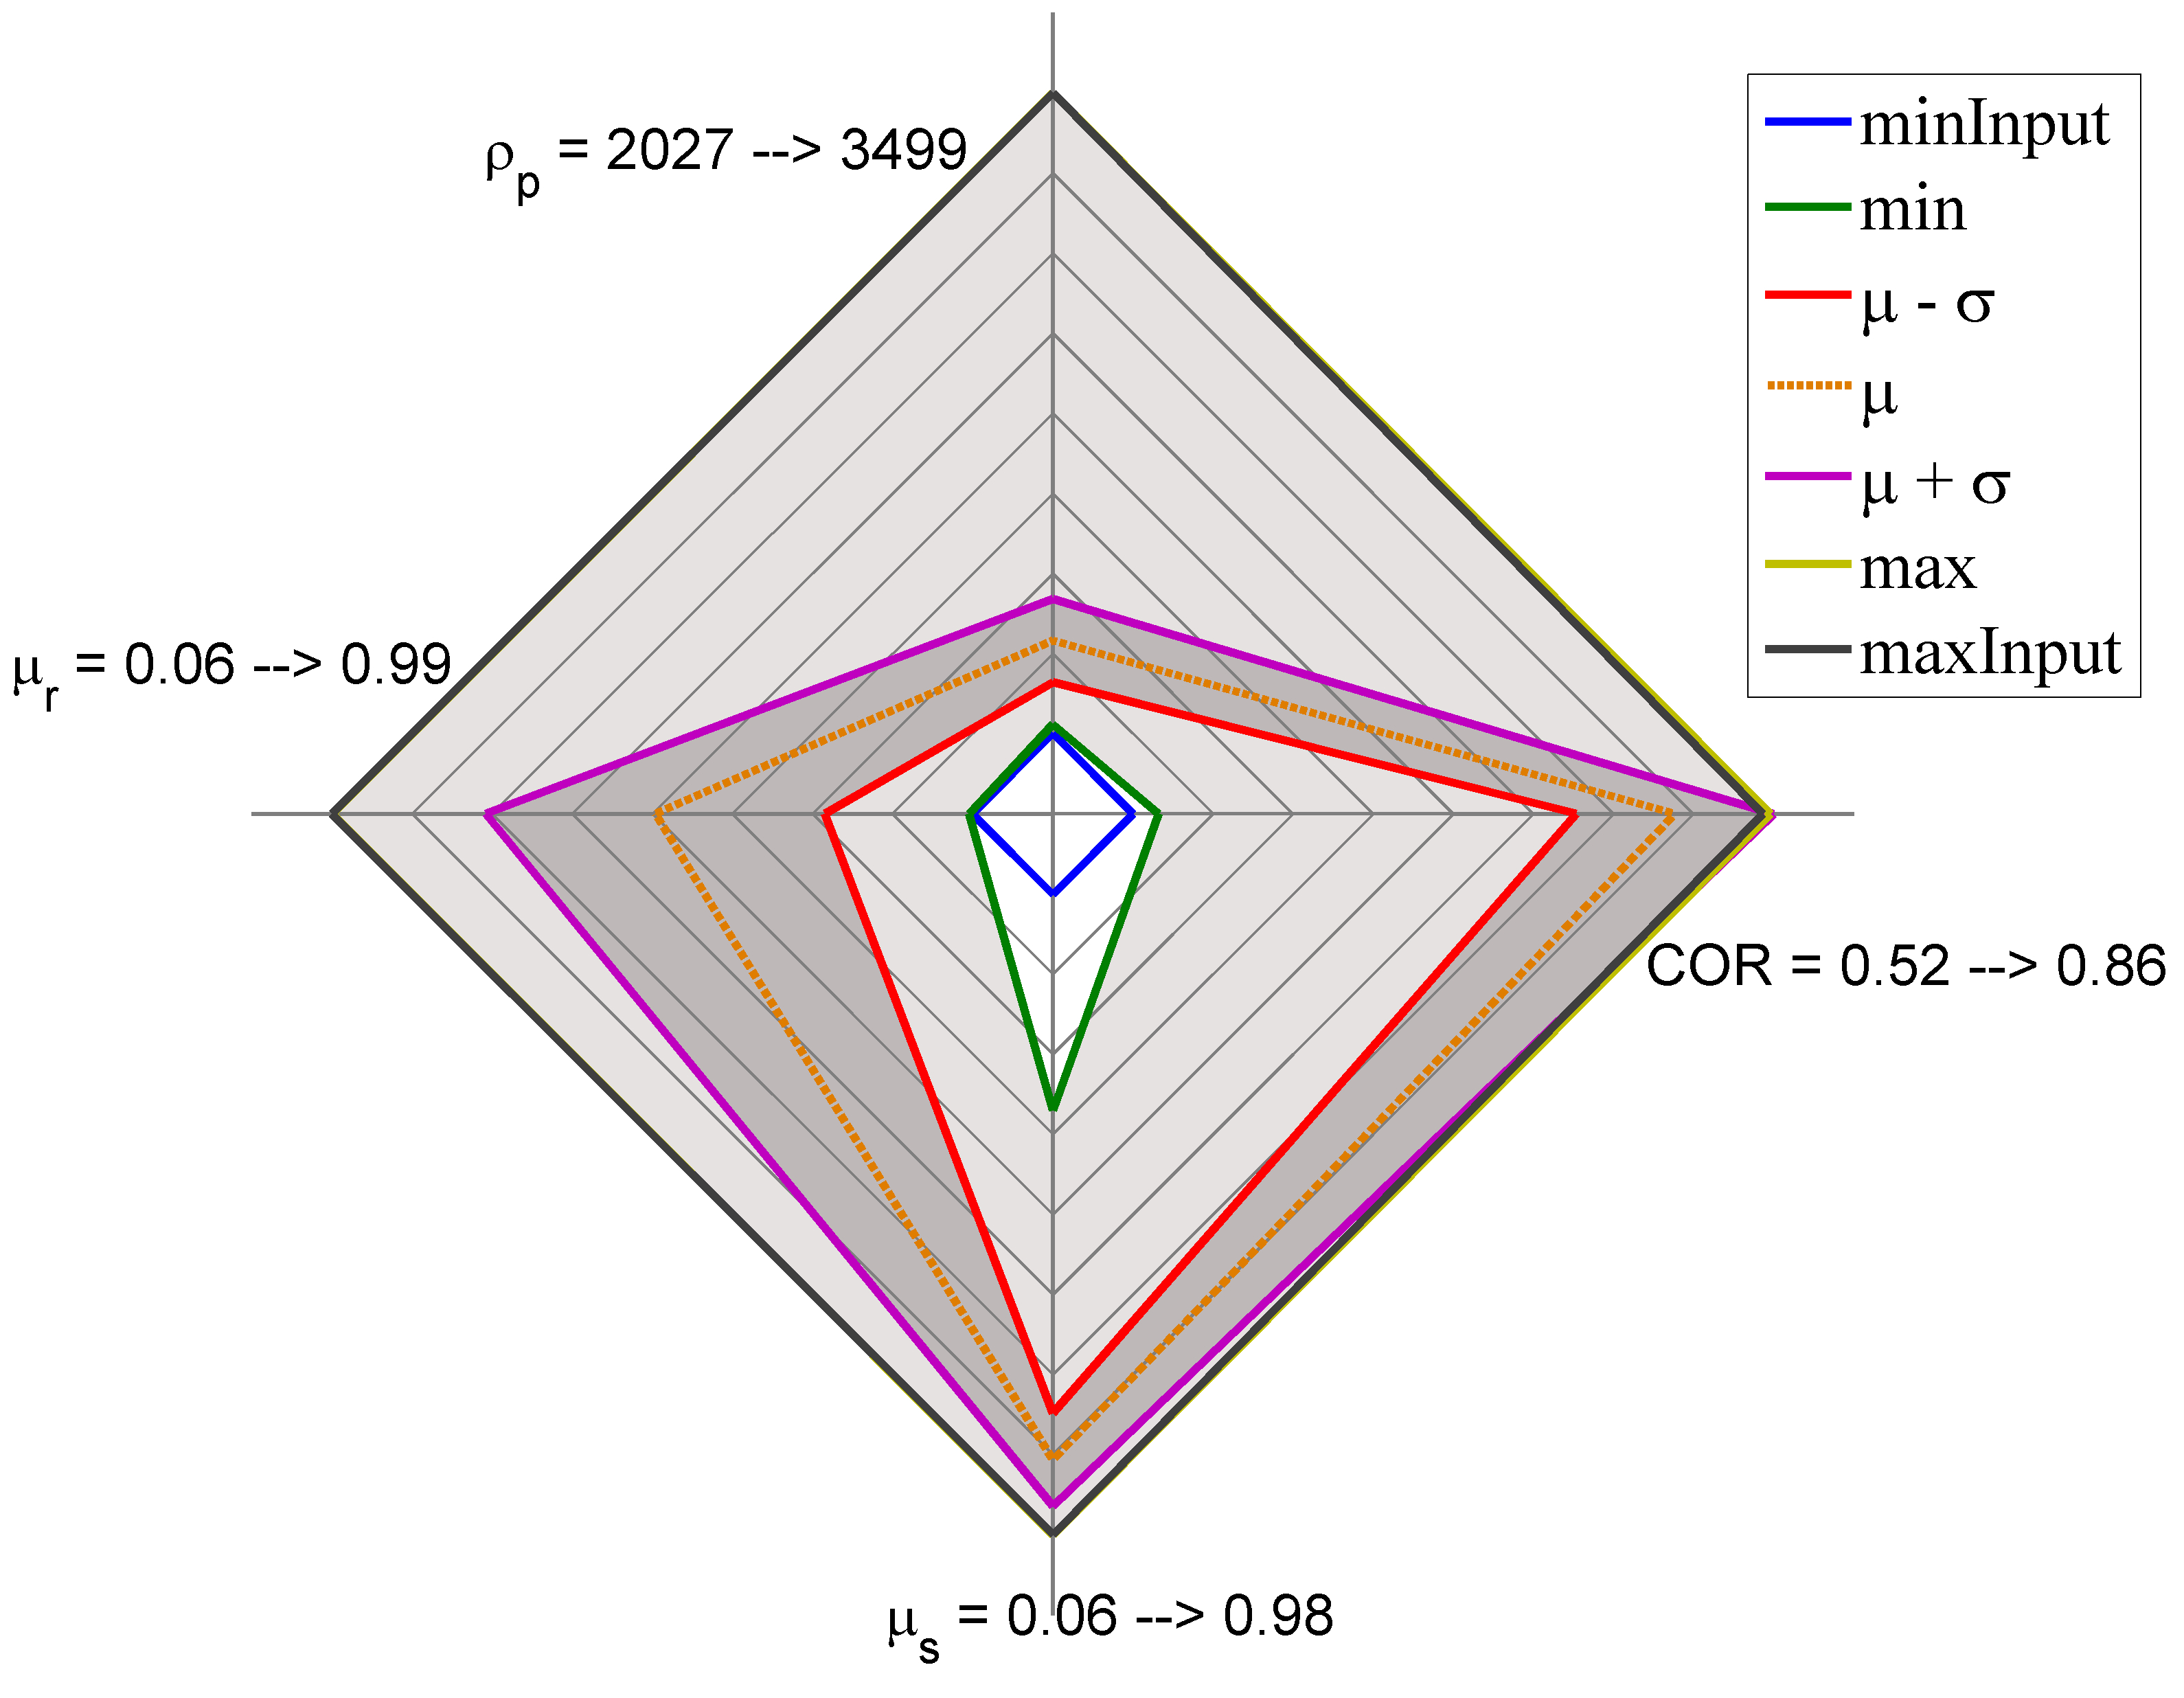
\includegraphics[height=3in]{images/original/28radarpirker12schulze10070}
%[width=.96\textwidth]
\caption{Radar P12 Schulze10070}
\label{fig:28radarpirker12schulze10070} 
\end{figure}

%SCT: sn = 10070 [Pa], coeff. P. = 1.2
% \begin{figure}[htp]
%     \centering
%     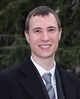
\includegraphics[width=.2\textwidth]{images/vitae/lbenvenuti}
%     \caption{OpenMP, MPI, MPI/OpenMP Hybrid runs of Box in a box testcase on 32
%     cores. The OpenMP-only run suffers from limited memory bandwidth in
%     memory-bound algorithms inside of the Modify section of the code. MPI-only has
%     low averaged runtimes for each section, but a very large Other timing, which
%     hints for a large amount of load-imbalance. Hybrid timings are a bit worse
%     on average, but because of better balancing, processes have lower wait times
%     inside of Other timing.}
% 	\label{fig:boxInBoxComparison}

% \ref{eq:rsquare}.
% \begin{equation}
R^2 = \frac {SSR}{SST} = 1 - \frac {SSE}{SST} .
 \label{eq:rsquare}
\end{equation}

% 
% \ref{eq:rootMeanSquareError}.
% \begin{equation}
RMSE = \sqrt{\frac{\sum _{i=1}^{n} (x_{i}-\widehat{x}_{i})^{2}}{n}}
\label{eq:rootMeanSquareError}
\end{equation}



% \lipsum[1]
% \begin{equation}
m \ddot{x}_{ij} + c \dot{x}_{ij} + k x_{ij} =  F_{ij} .
\label{equ:newtonlaw}
\end{equation}

% \subsection{ANN identification}
% \label{subsec:annmodeliden}
% \subsection{ANN application}
% \label{subsec:annapplication}
% 
% Later, each of these three trained $NN$ received as insertion $100M$ different
% combinations $DEM-micro$ parameters.
% So, we gained the numerical bulk behavior for each of this combination. 
% We then compared the values of these behaviors against the experimental bulk
% values, $SRSCT$ and $AOR$, obtaining a narrow range of valid DEM-micro
% combinations (about 80K).
% These results have been showed through radar plots (Figs. \ref{fig:15Schulze}
% and \ref{fig:16aorSchulzeIntersectionWorking}).
% To highlight an eventual $clumping$ behavior, we also plot the results in a
% cloud shape, see Fig. \ref{fig:17aorSchulzeIntersectionCloudSFRFCOR}.
% 
% %\begin{figure}[!htb] 
\centering 
\includegraphics[width=1.0\textwidth]{images/original/14aorSchulzeIntersection} 
\caption{aor Schulze Intersection}
\label{fig:14aorSchulzeIntersection} 
\end{figure}


% \begin{figure}[htp]
%     \centering
%     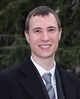
\includegraphics[width=.2\textwidth]{images/vitae/lbenvenuti}
%     \caption{OpenMP, MPI, MPI/OpenMP Hybrid runs of Box in a box testcase on 32
%     cores. The OpenMP-only run suffers from limited memory bandwidth in
%     memory-bound algorithms inside of the Modify section of the code. MPI-only has
%     low averaged runtimes for each section, but a very large Other timing, which
%     hints for a large amount of load-imbalance. Hybrid timings are a bit worse
%     on average, but because of better balancing, processes have lower wait times
%     inside of Other timing.}
% 	\label{fig:boxInBoxComparison}

% \begin{figure}[!htb] 
\centering 
\includegraphics[width=.8\textwidth]{images/original/15Schulze} 
\caption{aor Schulze Intersection}
\label{fig:14aorSchulzeIntersection} 
\end{figure}


% \begin{figure}[htp]
%     \centering
%     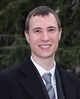
\includegraphics[width=.2\textwidth]{images/vitae/lbenvenuti}
%     \caption{OpenMP, MPI, MPI/OpenMP Hybrid runs of Box in a box testcase on 32
%     cores. The OpenMP-only run suffers from limited memory bandwidth in
%     memory-bound algorithms inside of the Modify section of the code. MPI-only has
%     low averaged runtimes for each section, but a very large Other timing, which
%     hints for a large amount of load-imbalance. Hybrid timings are a bit worse
%     on average, but because of better balancing, processes have lower wait times
%     inside of Other timing.}
% 	\label{fig:boxInBoxComparison}

% % \lipsum[1]
% \begin{figure}[!htb] 
\centering 
\includegraphics[width=.96\textwidth]{images/original/16aorSchulzeIntersectionWorking} 
\caption{aor Schulze Intersection working}
\label{fig:16aorSchulzeIntersectionWorking} 
\end{figure}


% \begin{figure}[htp]
%     \centering
%     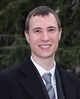
\includegraphics[width=.2\textwidth]{images/vitae/lbenvenuti}
%     \caption{OpenMP, MPI, MPI/OpenMP Hybrid runs of Box in a box testcase on 32
%     cores. The OpenMP-only run suffers from limited memory bandwidth in
%     memory-bound algorithms inside of the Modify section of the code. MPI-only has
%     low averaged runtimes for each section, but a very large Other timing, which
%     hints for a large amount of load-imbalance. Hybrid timings are a bit worse
%     on average, but because of better balancing, processes have lower wait times
%     inside of Other timing.}
% 	\label{fig:boxInBoxComparison}

% % \begin{equation}
\begin{aligned}
\phi_{e-psh} &= \arctan \left(\frac{\tau_{psh}}{\sigma_{n,psh}} \right) ,\\
\mu_{psh} &=\tan(\phi_{e-psh}) .
\end{aligned}
 \label{eq:phi_ps}
\end{equation}

% \begin{figure}[!htb] 
\centering 
\includegraphics[width=.96\textwidth]{images/original/17aorSchulzeIntersectionCloudSFRFCOR} 
\caption{Cloud aor Schulze Intersection working}
\label{fig:17aorSchulzeIntersectionCloudSFRFCOR} 
\end{figure}


% \begin{figure}[htp]
%     \centering
%     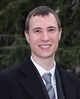
\includegraphics[width=.2\textwidth]{images/vitae/lbenvenuti}
%     \caption{OpenMP, MPI, MPI/OpenMP Hybrid runs of Box in a box testcase on 32
%     cores. The OpenMP-only run suffers from limited memory bandwidth in
%     memory-bound algorithms inside of the Modify section of the code. MPI-only has
%     low averaged runtimes for each section, but a very large Other timing, which
%     hints for a large amount of load-imbalance. Hybrid timings are a bit worse
%     on average, but because of better balancing, processes have lower wait times
%     inside of Other timing.}
% 	\label{fig:boxInBoxComparison}

